\newcommand{\eqtext}[2][4.5in]{\parbox{#1}{#2}}

\chapter{Classical mechanics}

The standard view in physics is that classical mechanics is perfectly understood. It has three different but equivalent formulations, the oldest of which, Newtonian mechanics, is based on three laws. Classical mechanics is the theory of point particles that follow those laws. Unfortunately, this view is incorrect.

We will see that the three formulations are not equivalent, in the sense that there are physical systems that are Newtonian but not Hamiltonian and vice-versa. There are also a number of questions that have been left unanswered, such as the precise nature of the Hamiltonian or the Lagrangian, and what exactly the principle of stationary action represents physically. While shedding light on these issues, we will also find that classical mechanics already contains elements that are typically associated with other theories, such as quantum mechanics/field theories (uncertainty principle, anti-particles), thermodynamics/statistical mechanics (thermodynamic and information entropy conservation) or special relativity (energy as the time component of a four-vector). In other words, the common understanding of classical mechanics is quite shallow, and its foundations are, in fact, not separate from the ones of classical statistical mechanics or special relativity.

What reverse physics shows is that the central assumption underneath classical mechanics is that of \textbf{infinitesimal reducibility (IR)}: a classical system can be thought of as made of parts, which in turn are made of parts and so on; studying the whole system is equivalent to studying all its infinitesimal parts. This assumption, together with the assumption of \textbf{independence of degrees of freedom (IND)}, is what gives us the structure of classical phase space with conjugate variables. The additional assumption of \textbf{determinism and reversibility (DR)}, the fact that the description of the system at one time is enough to predict its future or reconstruct its past, leads us to Hamiltonian mechanics. On the other hand, assuming \textbf{kinematic equivalence (KE)}, the idea that trajectories in space are enough to reconstruct the state of the system and vice-versa, leads to Newtonian mechanics. The combination of all above assumptions, instead, leads to Lagrangian mechanics and, in particular, to massive particles under (scalar and vector) potential forces.

As a guide to the chapter, here is the list of main points in the order in which they will be presented, one for each section.
\begin{enumerate}
	\item Review of classical formulations
	\item Lagrangian mechanics is Hamiltonian mechanics and KE
	\item Kinematics, in general, is not enough to reconstruct dynamics
	\item Hamiltonian mechanics (one DOF) is equivalent to DR
	\item Hamiltonian mechanics (multiple DOF) is equivalent to DR plus IND
	\item Differential calculus and its generalization, differential topology, study infinitesimally additive quantities that depend on geometric shapes (i.e. lines, surfaces, volumes)
	\item The principle of least action is a consequence of DR, IND and KE
	\item Massive particles under potential forces are a consequence of DR, IND and KE
	\item Special relativity is a consequence of DR, IND and KE
	\item Phase space is the only structure that makes distributions, state counting and entropy frame invariant
	\item Newtonian mechanics is a consequence of KE
	\item Three dimensional spaces are the only spaces for which distributions over directions are frame invariant
	\item Classical particle states as points in phase space are equivalent to IR
\end{enumerate}

\section{Formulations of classical mechanics}

In this section we will briefly review the three main formulations of classical mechanics. Our task is not to present them in detail, but rather to provide a brief summary of the equations so that we can proceed with the comparison. In particular, given that different conventions are used across formulations, within the same formulation and among different contexts (e.g. relativity, symplectic geometry), we will want to make the notation homogeneous to allow easier comparisons.

\subsection{Newtonian mechanics}

For all formulations, the system is modeled as a collection of point particles, though we will mostly focus on the single particle case. For a Newtonian system, the state of the system at a particular time $t$ is described by the position $x^i$ and velocity $v^i$ of all its constituents. Each particle has its mass $m$, not necessarily constant in time, and, for each particle, we define kinetic momentum as $\Pi^i = m v^i$.\footnote{We will use the letter $t$ for the time variable, $x$ for position and $v$ for velocity, which is a very common notation in Newtonian mechanics. However, we will keep using the same letters in Lagrangian mechanics as well, instead of $q$ and $\dot{q}$, for consistency. Given that the distinction between kinetic and conjugate momentum is an important one, we will denote $\Pi$ the former and $p$ the latter. The Roman letters $i,j,k,...$ will be used to span the spatial components (e.g. $i \in \{1,2,3\}$ for a particle in 3 dimensional space and $i \in \{1,2,\dots, 3n\}$ for n particles), while we will use the Greek letters $\alpha, \beta, \gamma, ...$ to span space-time components (e.g. $\alpha \in \{0,1,2,3\}$ where the $0$ value of the index is used for time). Unlike some texts, $x^i$ do not represent Cartesian coordinates, and therefore they should be understood already as generalized coordinates.}

The evolution of our system is given by Newton's second law:\footnote{For derivatives, we will use the shorthand $d_t$ for $\frac{d}{dt}$ and $\partial_{x^i}$ for $\frac{\partial}{\partial x^i}$. For functions that depend on multiple arguments we use a free index to note that it depends on all elements; each argument will have a different index to highlight that there is no relationship between arguments. }
\begin{equation}\label{rp-cm-NewtonsSecondLaw}
	F^i(x^j, v^k, t) = d_t \Pi^i.
\end{equation}
Mathematically, if the forces $F^i$ are locally Lipschitz\footnote{Lipschitz continuity means that the slope of the function is bounded. For example, $\sqrt{x}$ in the neighborhood of $0$ is not Lipschitz continuous as it has a vertical asymptote at that point. One can construct examples (e.g. Norton's dome) where the forces are not locally Lipschitz continuous, and therefore the initial position and velocity do not yield a unique solution (i.e. in Norton's dome, the body can stay on the top of the dome indefinitely, or it can fall down after an arbitrary amount of time). In this case, something else, outside the system, will necessarily determine what is the motion of the system, and therefore it is not true that the force and the state of the system fully determine the dynamics of the system.} continuous, then the solution $x^i(t)$ is unique. That is, given position and velocity at a given time, we can predict the position and velocity at future times. We will assume a Newtonian system has this property.

An important aspect of Newtonian mechanics is that the equations are not invariant under coordinate transformation. To distinguish between apparent forces (i.e. those dependent on the choice of frame) and the real ones, we assume the existence of inertial frames. In an inertial frame there are no apparent forces, and therefore a free system (i.e. no forces) with constant mass proceeds in a linear uniform motion, or stays still.\footnote{Recall that linear motion simply means that it describes a line in space, while uniform motion means that the speed is constant. Therefore we can have linear non-uniform notion (e.g. an object accelerated along the same direction) or a non-linear uniform motion (e.g. an object going around in a circle at constant speed).}

\subsection{Lagrangian mechanics}

The state for a Lagrangian system is also given by position $x^i$ and velocity $v^i$. The dynamics is specified by a single function $L(x^i, v^j, t)$ called the Lagrangian. For each spatial trajectory $x^i(t)$ we define the action as $\mathcal{A}[x^i(t)] = \int_{t_0}^{t_1} L(x^i(t), d_t x^i(t), t) dt$. The trajectory taken by the system is the one that makes the action stationary:
\begin{equation}
\delta \mathcal{A}[x^i(t)] = \delta \int_{t_0}^{t_1} L\left(x^i(t), d_t x^i(t), t\right) dt=0
\end{equation}
The evolution can equivalently be specified by the Euler-Lagrange equations:
\begin{equation}\label{rp-cm-EulerLagrange}
	\partial_{x^i}L=d_t \partial_{v^i} L.
\end{equation}

Note that not all Lagrangians lead to a unique solution. For example, $L=0$ will give the same action for all trajectories and therefore, strictly speaking, all trajectories are possible. The stationary action leads to a unique solution if and only if the Lagrangian is hyperregular, which means the Hessian matrix $\partial_{v^i}\partial_{v^j} L$ is invertible. Like in the Newtonian case, we will assume Lagrangian systems satisfy this property.

Unlike Newton's second law, both the Lagrangian and the Euler-Lagrange equations are invariant under coordinate transformations. This means that Lagrangian mechanics is particularly suited to study the symmetries of the system.

\subsection{Hamiltonian mechanics}

In Hamiltonian mechanics, the state of the system is given by position $q^i$ and conjugate momentum $p_i$. The dynamics is specified by a single function $H(q^i, p_j, t)$ called the Hamiltonian.\footnote{We use a different symbol for position in Hamiltonian mechanics because, while it is true that $q^i = x^i$, it is also true that $\partial_{q^i} \neq \partial_{x^i}$: the first derivative is taken at constant conjugate momentum while the second is taken at constant velocity. This creates absolute confusion when mixing and comparing Lagrangian and Hamiltonian concepts, which our notation avoids completely.} The evolution is given by Hamilton's equations:
\begin{equation}\label{rp-cm-HamiltonEq}
	\begin{aligned}
		d_t q^i = \partial_{p_i} H \\
		d_t p_i = - \partial_{q^i} H \\
	\end{aligned}
\end{equation}
We will again want these equations to yield a unique solution, which means the Hamiltonian must be at least differentiable, and the derivatives must at least be Lipschitz continuous.

Hamilton's equations are invariant as well. The Hamiltonian itself is a scalar function which is often considered (mistakenly as we'll see later) invariant. This formulation is the most suitable for statistical mechanics as volumes of phase space correctly count the number of possible configurations.

\section{Inequivalence of formulations}\label{rp-cm-inequivalenceOfFormulations}

It is often stated in physics books that all three formulations of classical mechanics are equivalent. We will look at this claim in detail, and conclude that this is not the case: there are systems that can be described by one formulation and not another. More precisely, the set of Lagrangian systems is exactly the intersection of Newtonian and Hamiltonian systems.

\subsection{Testing equivalence}

We will consider two formalisms equivalent if they can be applied to exactly the same systems. That is, Newtonian and Lagrangian mechanics are equivalent if any system that can be described using Newtonian mechanics can also be described by Lagrangian mechanics and vice-versa. In general, in physics great emphasis is put on systems that can indeed be studied by all three, leaving the impression that this is always doable.\footnote{If one asks the average physicist whether Newtonian and Hamiltonian mechanics are equivalent, the answer most of the time will be  enthusiastically positive. If one then asks for the Hamiltonian for a damped harmonic oscillator, the typical reaction is annoyance due to the nonsensical question (damped harmonic oscillators do not conserve energy), followed by a realization and partial retraction of the previous claim. The moral of the story is to never take these claims at face value.} However, just with a cursory glance, we realize that this can't possibly be the case.

The dynamics of a Newtonian system, in fact, is specified by three independently chosen functions of position and velocity, the forces applied to each degree of freedom. On the other hand, the dynamics of Lagrangian and Hamiltonian systems is specified by a single function of position and velocity/momentum, the Lagrangian/Hamiltonian. Intuitively, there are more choices in the dynamics for Newtonian systems than for Lagrangian and Hamiltonian.

Now, the reality is a bit trickier because the mathematical expression of the forces is not enough to fully characterize the physical system. We need to know in which frame we are, what coordinates are being used and the mass of the system, which is potentially a function of time. On the Lagrangian side, note that the Euler-Lagrange equations are homogeneous in $L$. This means that multiplying $L$ by a constant leads to the same solutions, meaning that the same system can be described by more than one Lagrangian. The converse is also true: if one system is half as massive and is subjected to a force half as intense, the resulting Lagrangian is also simply rescaled by a constant factor. Therefore the map between Lagrangians and Lagrangian systems is not one-to-one: it is many-to-many. This is why we should never look simply at mathematical structures if we want to fully understand the physics they describe.

Regardless, our task is at the moment much simpler: we only need to show that there are Newtonian systems not expressible by Lagrangian or Hamiltonian mechanics. We can therefore limit ourselves to systems with a specific constant mass $m$ in an inertial frame and write $a^i=F^i(x^j, v^k, t)/m$. Given that the force is arbitrary, the acceleration can be an arbitrary function of position, velocity and time. Similarly, we can write the acceleration of a Lagrangian system as $a^i=F^i[L]/m$. That is, the acceleration is going to be some functional of the Lagrangian. Given the Euler-Lagrange equations \ref{rp-cm-EulerLagrange}, the map between the Lagrangian and the acceleration must be continuous in both direction: for small variation of the Lagrangian we must have a small variation of the equations of motion and therefore of the acceleration, and for small variations of the equations of motions we must have a small variation of the Lagrangian. But a continuous surjective map from the space of a single function (i.e. the Lagrangian) to the space of multiple functions (i.e. those that specify the acceleration in terms of position and velocity) does not exist,\footnote{Mathematically, the space of continuous functions $C(\mathbb{R}, \mathbb{R})$ and $C(\mathbb{R}^n, \mathbb{R})$ are not homeomorphic. Intuitively, the underlying reason is the same as to why a map from a volume to a line can't be continuous: in a volume you have infinitely many directions you can move away from a point, while on a line you only have two.} and therefore there must be at least one Newtonian system with constant mass expressed in an inertial frame that is not describable using Lagrangian mechanics. The same argument applies for Hamiltonian mechanics, since the dynamics in this case is also described by a single function in the same number of arguments. We therefore reach the following conclusion:
\begin{insight}
	Not all Newtonian systems are Lagrangian and/or Hamiltonian.
\end{insight}

\subsection{Newtonian vs Lagrangian/Hamiltonian}

We now want to understand whether all Lagrangian systems are Newtonian. Given what we discussed, we cannot expect to reconstruct the mass and force uniquely from the expression of the Lagrangian. We consider the mass and the frame fixed by the problem, together with the Lagrangian, and therefore we must only see whether we can indeed find a unique expression for the acceleration. From the Euler-Lagrange equations \ref{rp-cm-EulerLagrange} we can write
\begin{equation}
	\begin{aligned}
	\partial_{x^i}L&=d_t \partial_{v^i} L=\partial_{x^j} \partial_{v^i} L \, d_t x^j + \partial_{v^k} \partial_{v^i} L \, d_t v^k = \partial_{x^j} \partial_{v^i} L \, v^j + \partial_{v^k} \partial_{v^i} L \, a^k \\
	\partial_{v^k} &\partial_{v^i} L \, a^k = \partial_{x^i}L - \partial_{x^j} \partial_{v^i} L \, v^j .
	\end{aligned}
\end{equation}
To be able to write the acceleration explicitly, we must be able to invert the Hessian matrix $\partial_{v^k} \partial_{v^i} L$. As we noted before, this is exactly the condition for which the principle of stationary action leads to a unique solution, and we can better understand why. If it is not invertible at a point, the determinant is zero and therefore one eigenvalue is zero. The corresponding eigenvector corresponds to a direction for which the equation tells us nothing, and therefore a variation of the acceleration in that direction will not change the action. This is why the invertibility of the Hessian is required in order to obtain unique solutions.

What we find, then, is that for any Lagrangian system, which we assume to have a unique solution, we can explicitly write the acceleration as a function of position, velocity and time. Therefore
\begin{insight}
	All Lagrangian systems are Newtonian.
\end{insight}

Now we turn our attention to Hamiltonian mechanics and, similarly, we ask whether we can express the acceleration as a function of position and velocity. We have
\begin{equation}
	\begin{aligned}
		a^i &= d_t v^i = d_t d_t q^i = d_t \partial_{p_i} H = \partial_{q^j} \partial_{p_i} H d_t q^j + \partial_{p_k} \partial_{p_i} H d_t p_k \\
		&= \partial_{q^j} \partial_{p_i} H \partial_{p_j} H - \partial_{p_k} \partial_{p_i} H \partial_{q^k} H.
	\end{aligned}
\end{equation}
This tells us that the acceleration is always an explicit function, but it is, in general, an explicit function of position and momentum, not of position and velocity. To change the expression, we need to be able to write the momentum as a function of position and velocity. Note that Hamilton's equations already give a way to express the velocity in terms of position and momentum, we just need that expression to be invertible, which means the Jacobian must be invertible. We must have:
\begin{equation}
	\left|\partial_{p_i} v^j\right| = \left|\partial_{p_i}\partial_{p_j} H\right| \neq 0 .
\end{equation}
To be able to express momentum as a function of position and velocity, then, we need the Hessian of the Hamiltonian to be invertible (i.e. to have non-zero determinant).

Note that we had no such requirement for the Hamiltonian. For example, $H=0$ leads to equations $d_t q^i = 0$ and $d_t p_i = 0$, which have unique solutions: both position $q^i(t) = k_{q^i}$ and momentum $p_i(t) = k_{p_i}$ are constants of motion. The Hessian, being the zero matrix, is not invertible, and in fact we cannot write momentum as a function of position and velocity: velocity $d_t q^i$ is always zero in all cases while conjugate momentum can be any value $k_{p_i}$. Though this case may not be physically interesting, it is a perfectly valid Hamiltonian system and shows that we should always check the trivial mathematical case. However, let us go through a more physically meaningful case.

\begin{figure}
	\centering
	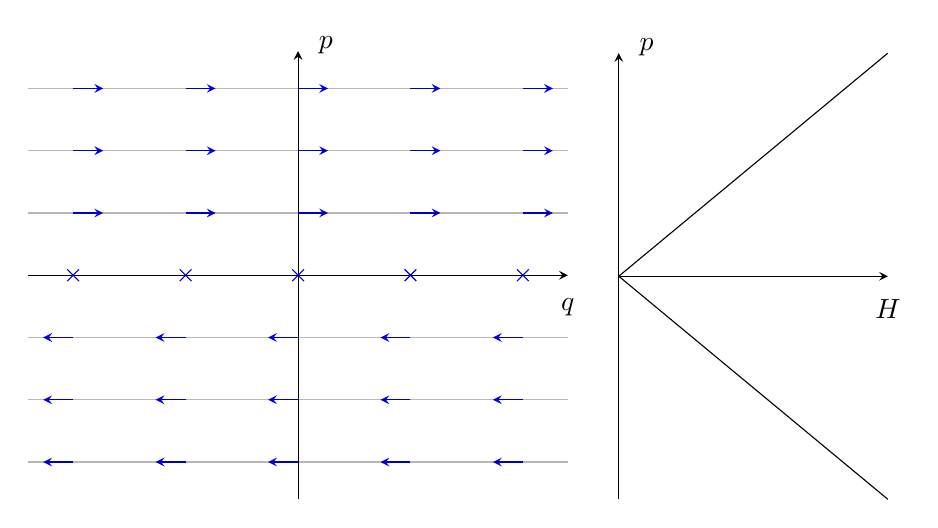
\begin{tikzpicture}
		%TODO: different thickness/color for the Hamiltonian and the axis
		\pgfplotsset{ticks=none}
		\begin{axis}[axis lines=middle,
			xlabel=$q$,
			xlabel style={below=5pt, fill=white},
			ylabel=$p$,
			ylabel style={above=2pt, right=4pt},
			domain=-1.5:1.5,
			ymin=-1.8, ymax=1.8,]
			\foreach \yvalue in {-1.5,-1,-0.5, 0.5, 1, 1.5} {
				\addplot[blue,-stealth,samples=5,
				quiver={
					u={y/abs(y)},
					v={0},
					scale arrows=0.2},
				] {\yvalue};
				\addplot[black,samples=2,opacity=0.2,domain=-1.8:1.8]{\yvalue};
				\addplot[black,samples=2,opacity=0.1.5,domain=-1.8:1.8]{\yvalue};}
			\addplot[scatter, only marks, mark size=3pt, samples=5, mark=x, color=green]{0};
		\end{axis}
		
		\pgfplotsset{ticks=none}
		\begin{axis}[
			xshift=7.5cm,
			width=5cm,
			height=7.25cm,				
			axis lines=middle,
			xlabel=$H$,
			xlabel style={below=5pt, fill=white},
			ylabel=$p$,
			ylabel style={above=2pt, right=4pt},
			domain=0:1,
			xmin=0, xmax=1,
			ymin=-1, ymax=1,]
			\addplot[black,samples=2,domain=0:1]{x};
			\addplot[black,samples=2,domain=0:1]{-x};
		\end{axis}
	\end{tikzpicture}
	\caption {On the left, the phase space diagram for a photon treated as a point particle. The Hamiltonian $H=c|p|$, on the right, is proportional to the modulus of $p$. Since $H$ is not differentiable when $p=0$, those states are excluded, consistent with the physics. The displacement field has only a $q$ component, which is $+c$ above the horizontal axis and $-c$ below the horizontal axis. } \label{fig_rp_cm_photon}
\end{figure}

\textbf{Photon as a particle}. If we want to treat the photon as a classical particle, we can write the Hamiltonian by expressing the energy as a function of momentum
\begin{equation}
	H=\hbar | \omega| = c \hbar |k| = c |p|.
\end{equation}
If we apply Hamilton's equations, we have
\begin{equation}
	\begin{aligned}
		d_t q^i &= c \frac{p^i}{|p|} \\
		d_t p_i &= 0.
	\end{aligned}
\end{equation}
That is, the norm of the velocity is always $c$, the momentum decides its direction, and the momentum itself does not change in time, as shown in fig. \ref{fig_rp_cm_photon}. This is indeed the motion of a free photon. One can confirm, through tedious calculation, that the determinant of the Hessian is indeed zero, yet it is easier and more physically instructive to see that we cannot reconstruct the momentum from the velocity. Relativistically, all photons travel along the geodesics at the same speed, therefore two photons that differ only by the magnitude of the momentum will travel the same path.

Hamiltonian systems that are also Newtonian, then, need to satisfy this extra condition, so let us give it a name.
\renewcommand{\theassump}{KE}
\begin{assump}[Kinematic Equivalence]\label{assum_kineq}
	The kinematics of the system is sufficient to reconstruct its dynamics and vice-versa. That is, specifying the motion of the system is equivalent to specifying its state and evolution.
\end{assump}
\renewcommand{\theassump}{\Roman{assump}}
By kinematics we mean the motion in space and time and by dynamics we mean the state and its time evolution in phase space. We will need to analyze the difference between the two more in detail, but we should first finish our comparison between the different formulations.

Summing up, we find that
\begin{insight}
	Not all Hamiltonian systems are Newtonian: only those for which  \ref{assum_kineq} is valid.
\end{insight}

\subsection{Lagrangian vs Newtonian}

We now need to compare Lagrangian and Hamiltonian systems. The task is a lot easier because we already have a precise way to connect the two. If we are given a Lagrangian $L$, we define the conjugate momentum $p_i = \partial_{v^i} L$ and the Hamiltonian $H = p_i v^i - L$. If we are given a Hamiltonian $H$, we can define a Lagrangian $L = p_i v^i - H$ and a velocity $v^i = d_t q^i = \partial_{p_i} H$. The only detail that needs to be understood is whether this can be done for all Lagrangian and Hamiltonian systems.

While these expressions are always defined, we need to check whether we can change variables; whether we can write the Lagrangian in terms of position and velocity and the Hamiltonian in terms of position and momentum. Going from a Hamiltonian to a Lagrangian, it again means that we can write momentum as a function of position and velocity, and therefore assumption \ref{assum_kineq} must hold. This makes sense: if all Lagrangian systems are Newtonian, and \ref{assum_kineq} was required for a Hamiltonian system to be Newtonian, then it is also required for a Hamiltonian system to be Lagrangian. But the connection is stronger: \ref{assum_kineq} is the \emph{only} additional assumption we need to be able to write a Lagrangian given a Hamiltonian.

Going from a Lagrangian to a Hamiltonian, it means that we can write velocity as a function of position and momentum. Note that since we define conjugate momentum as the derivative of the Lagrangian, we can already express momentum as a function of position and velocity, which means we are simply asking that expression to be invertible. This is, again, assumption \ref{assum_kineq}, just in the opposite direction. We must have
\begin{equation}
	0 \neq \left| \partial_{v^i} p_j \right| = \left| \partial_{v^i} \partial_{v^j} L \right|.
\end{equation}
This means that assumption \ref{assum_kineq} is exactly the invertibility of the Hessian, the condition for unique solution of the Lagrangian. All Lagrangian systems that admit unique solutions, then, satisfy assumption \ref{assum_kineq}. In fact, we can see that the Hessian determinants are related
\begin{equation}
	\left| \partial_{v^i} \partial_{v^j} L \right| = \left| \partial_{v^i} p_j \right| = \left| \partial_{p_i} v^j \right|^{-1} = \left|\partial_{p_i}\partial_{p_j} H\right|^{-1}.
\end{equation}
This means that every Lagrangian admits a Hamiltonian, but not every Hamiltonian admits a Lagrangian. Only the Hamiltonian systems for which \ref{assum_kineq} is valid will also be Lagrangian systems, with a guaranteed unique solution given that \ref{assum_kineq} is exactly the assumption needed for that as well. Therefore we conclude that
\begin{insight}
	Lagrangian systems are exactly those Hamiltonian systems for which \ref{assum_kineq} is valid.
\end{insight}

\subsection{Relationship between formulations}

The relationship between the different formulations, then, can be summarized with the Venn diagram in fig. \ref{rp-cm-fig-vennDiagramEarly}.

\begin{figure}[h]
	\centering
	\begin{tikzpicture}
		\node[ellipse, minimum width=10cm, minimum height=5cm, draw, left] (ns){};
		\node [align=left, above] at ([xshift=-6mm,yshift=1mm]ns.north west) {Newtonian \\systems};
		
		\node[ellipse, minimum width=6cm, minimum height=4.5cm, draw] (hs) at ([xshift=-1.7cm]ns.east){};
		\node [align=right, above right] at ([xshift=8mm, yshift=-4mm]hs.north) {Hamiltonian\\ systems};
		\node [align=center, right] at ([xshift=14
		mm]hs.west) {Lagrangian \\systems};
	\end{tikzpicture}
	\caption {Not all Hamiltonian systems are Newtonian and not all Newtonian systems are Hamiltonian. All Lagrangian systems are both Newtonian and Hamiltonian.}\label{rp-cm-fig-vennDiagramEarly}
\end{figure}


We have found that \ref{assum_kineq} is a constitutive assumption of Lagrangian mechanics, and that it clearly marks which Hamiltonian systems are Newtonian/Lagrangian. By constitutive assumption we mean an assumption that must be taken, either explicitly or implicitly, for a theory to be valid. But what makes a system Hamiltonian and what makes a system Newtonian? Can we find a full set of constitutive assumptions for classical mechanics?

\section{Kinematics vs dynamics}

We have seen the importance of the connection between kinematics and dynamics. In this section we will explore this link more deeply and come to the following conclusion: the kinematics of a system is not enough to reconstruct its dynamics. 

\subsection{Particle under linear drag}

Let us first review exactly what the kinematics and dynamics are. Given a system, its kinematics is the description of its motion in space and time. Position, velocity, and acceleration are kinematic variables because they describe the motion. Kinematics is what Galileo studied and started to give a rigorous account of. The dynamics, instead, describes the cause of such motion. Force, mass, momentum, energy are dynamic quantities as they are used to describe why a body moves in a particular way. Dynamics is what Newton introduced and his second law, expressed as $F=ma$, clearly shows the link.

The link between the two concepts seems important given the constitutive role of \ref{assum_kineq} in Lagrangian mechanics. Moreover, while both Newtonian and Hamiltonian mechanics are dynamical theories, in the sense that quantities like force and momentum are intrinsic parts of the respective theories, Lagrangian mechanics seems to be a purely kinematic theory, as it is described only by kinematic variables like position and velocity. Therefore it seems useful to characterize the kinematics-dynamics link as much as possible. Let's analyze a concrete example.

Suppose we are given the following equation:
\begin{equation}\label{rp-cm-frictionEquation}
	m a = - b v .
\end{equation}
The equation is in terms of kinematic variables and, given initial conditions $x_0$ and $v_0$, it admits a unique solution, a unique trajectory.
The solution, plotted in fig. \ref{fig_rp_cm_dragEvolution}, is
\begin{equation}
	\begin{aligned}
	x(t)&= x_0 + v_0 \frac{m}{b} \left( 1 - e^{-\frac{b}{m}t}\right) \\
	v(t)&= v_0 e^{-\frac{b}{m}t} \\
	a(t)&= - v_0 \frac{b}{m} e^{-\frac{b}{m}t}
	\end{aligned}
\end{equation}
Can we reconstruct the forces acting on this system?

\begin{figure}
	\centering
	\begin{tikzpicture}
		\def\xi{0.25};
		\def\vi{1.25};
		\def\m{1};
		\def\b{1};
		\pgfplotsset{ticks=none}
		\begin{axis}[
			width=5.3cm,
			height=4.5cm,				
			axis lines=middle,
			axis line style={-},
			clip=false,
			xlabel=$t$,
			xlabel style={below=5pt},
			ylabel=$x$,
			ylabel style={above=2pt, left},
			xmin=0,xmax=4,
			ymin=0,ymax=2,
			domain=0:4,
			]
			\addplot[black,samples=30]{\xi + \vi*(\m/\b)*(1-exp((-\b/\m)*x))}
			node [pos=0,left] {$x_0$};
			\addplot[black,samples=2,dashed,opacity=0.5] {1.5}
			node [pos=0,left,opacity=1] {$x_0+ \frac{m}{b}v_0$};
		\end{axis}
		
		\begin{axis}[
			xshift=5cm,
			width=5.3cm,
			height=4.5cm,				
			axis lines=middle,
			axis line style={-},
			clip=false,
			xlabel=$t$,
			xlabel style={below=5pt},
			ylabel=$v$,
			ylabel style={above=2pt, left},
			xmin=0,xmax=4,
			ymin=0,ymax=1.7,
			domain=0:4,
			]
			\addplot[black,samples=30]{\vi*exp((-\b/\m)*x))}
			node [pos=0,left] {$v_0$};
			
		\end{axis}
		
		\begin{axis}[
			xshift=10cm,
			width=5.3cm,
			height=4.5cm,				
			axis lines=middle,
			axis line style={-},
			clip=false,
			xlabel=$t$,
			xlabel style={below=5pt},
			ylabel=$a$,
			ylabel style={above=2pt, left},
			xmin=0,xmax=4,
			ymin=-1.4,ymax=0.4,
			domain=0:4,
			]
			\addplot[black,samples=30]{-\vi*(\b/\m)*exp((-\b/\m)*x))}
			node [pos=0,left] {$-\frac{b}{m}v_0$};
			
		\end{axis}
	\end{tikzpicture}
	\caption {Evolution in time of position, velocity and acceleration for $ma = - bv$. Both acceleration and velocity will tend to zero as time increases. The position will tend to an equilibrium given by initial position and initial velocity.} \label{fig_rp_cm_dragEvolution}
\end{figure}

The obvious answer seems to be that the constant $m$ represents the mass of the system and $F = -bv$ the force. This is the case of a particle under linear drag:  the system is subjected to a frictional force that is proportional and opposite to the velocity. If we set the Lagrangian
\begin{equation}\label{rp-cm-frictionLagrangian}
	L = \frac{1}{2} m v^2 e^{\frac{b}{m}t}.
\end{equation}
and apply the Euler-Lagrange equation \ref{rp-cm-EulerLagrange} we have
\begin{equation}
	\begin{aligned}
	\partial_x L &= 0 = d_t \partial_v L = d_t \left(m v e^{\frac{b}{m}t} \right)=mae^{\frac{b}{m}t} + \frac{b}{m} m v e^{\frac{b}{m}t} = e^{\frac{b}{m}t}(ma + bv) \\
	ma &= - bv.
	\end{aligned}
\end{equation}
Therefore we have a Lagrangian for the system. We can also find a Hamiltonian
\begin{equation}\label{rp-cm-kd-momentumHamiltonian}
	\begin{aligned}
	p &= \partial_v L = m v e^{\frac{b}{m}t} \\
		v &= \frac{p}{m} e^{-\frac{b}{m}t} \\
		H &= p v - L = p \frac{p}{m} e^{-\frac{b}{m}t} - \frac{1}{2} m \left( \frac{p}{m} e^{-\frac{b}{m}t} \right)^2 e^{\frac{b}{m}t} = \frac{p^2}{m}  e^{-\frac{b}{m}t} - \frac{1}{2} \frac{p^2}{m}  e^{-\frac{b}{m}t} \\ 
		&=\frac{1}{2} \frac{p^2}{m}  e^{-\frac{b}{m}t}
	\end{aligned}
\end{equation}
and apply Hamilton's equations \ref{rp-cm-HamiltonEq}
\begin{equation}
	\begin{aligned}
		d_t q &= \partial_p H = \frac{p}{m}  e^{-\frac{b}{m}t} \\
		d_t p &= - \partial_q H = 0. 
	\end{aligned}
\end{equation}
The second equation tells us momentum is constant $p_0$. Substituting the constant in the first equation, we have the velocity as a function of time, which we can integrate. We have
\begin{equation}
	\begin{aligned}
	q(t) &= q_0 + \frac{p_0}{b} \left( 1 - e^{-\frac{b}{m}t}\right) \\
	p(t) &= p_0.
	\end{aligned}
\end{equation}

The kinematics works perfectly, but the dynamics seems off, as shown in fig. \ref{fig_rp_cm_dragDynamics}. First of all, based on the physics, one would expect the momentum to be decreasing in time
\begin{equation}
	p(t)=m v(t) = m v_0 e^{-\frac{b}{m}t}.
\end{equation}
However, conjugate momentum is a constant of motion. For the energy, we would expect the Hamiltonian to match the kinetic energy
\begin{equation}
	E(t)=\frac{1}{2} m v^2(t) = \frac{1}{2} m v_0^2 e^{-2\frac{b}{m}t}
\end{equation}
but if we express the Hamiltonian in terms of velocity we have
\begin{equation}
	H(t)=\frac{1}{2} \frac{p^2}{m} e^{-\frac{b}{m}t} = \frac{1}{2} \frac{1}{m} \left( m v(t) e^{\frac{b}{m}t} \right)^2 e^{-\frac{b}{m}t}= \frac{1}{2} m v^2(t) e^{\frac{b}{m}t} = \frac{1}{2} m v_0^2 e^{-\frac{b}{m}t}.
\end{equation}
That is, the energy decreases more slowly than it should. This is not good.

\begin{figure}
	\centering
	\begin{tikzpicture}
		\def\qi{0.25};
		\def\pi{1.25};
		\def\vi{1.25};
		\def\m{1};
		\def\b{1};
		\pgfplotsset{ticks=none}
		\begin{axis}[
			width=5.3cm,
			height=4.5cm,				
			axis lines=middle,
			axis line style={-},
			clip=false,
			xlabel=$t$,
			xlabel style={below=5pt},
			ylabel=$q$,
			ylabel style={above=2pt, left},
			xmin=0,xmax=4,
			ymin=0,ymax=2,
			domain=0:4,
			]
			\addplot[black,samples=30]{\qi + (\pi/\b)*(1-exp((-\b/\m)*x))}
			node [pos=0,left] {$q_0$};
			\addplot[black,samples=2,dashed,opacity=0.5] {1.5}
			node [pos=0,left,opacity=1] {$q_0+\frac{1}{b}p_0$};
		\end{axis}
		\begin{axis}[
			xshift=5cm,
			width=5.3cm,
			height=4.5cm,				
			axis lines=middle,
			axis line style={-},
			clip=false,
			xlabel=$t$,
			xlabel style={below=5pt},
			ylabel=$p$,
			ylabel style={above=2pt, left},
			xmin=0,xmax=4,
			ymin=0,ymax=1.7,
			domain=0:4,
			]
			\addplot[black,samples=30]{\m*\vi*exp((-\b/\m)*x)}
			node [pos=0.5,above=5pt] {$mv(t)$};
			\addplot[black,samples=30]{\pi}
			node [pos=0,left] {$p_0$}
			node [pos=0.5,above] {$p(t)$};
			
		\end{axis}
		
		\begin{axis}[
			xshift=10cm,
			width=5.3cm,
			height=4.5cm,				
			axis lines=middle,
			axis line style={-},
			clip=false,
			xlabel=$t$,
			xlabel style={below=5pt},
			ylabel=$E$,
			ylabel style={above=2pt, left},
			xmin=0,xmax=4,
			ymin=0,ymax=1,
			domain=0:4,
			]
			\addplot[black,samples=30]{0.5*\m*pow(\vi,2)*exp((-\b/\m)*2*x))}
			node [pos=0.3,below,left=1pt] {$E(t)$};
			\addplot[black,samples=30]{0.5*\m*pow(\vi,2)*exp((-\b/\m)*x))}
			node [pos=0,left] {$\frac{p_0^2}{2m}$}
			node [pos=0.4,above=5pt] {$H(t)$};
			
		\end{axis}
	\end{tikzpicture}
	\caption {Trying to interpret $L = \frac{1}{2} m v^2 e^{\frac{b}{m}t}$ and $H=\frac{1}{2} \frac{p^2}{m} e^{-\frac{b}{m}t}$ as respectively the Lagrangian and Hamiltonian of a particle under linear drag. While evolution of the position matches, note how the conjugate momentum is constant while the kinetic momentum decreases. Also, the Hamiltonian and the energy do not decrease at the same rate.} \label{fig_rp_cm_dragDynamics}
\end{figure}

Now, it is true that conjugate momentum is not the same as kinetic momentum. But the difference, as we will see much more clearly later, is caused by non-inertial non-Cartesian coordinate systems and/or the presence of vector potential forces.\footnote{The relationship is $p_i = m g_{ij} v^j + \mathfrak{q} A_i$. This reduces to $p_i = m v^i$ if and only if we are in an inertial frame with Cartesian coordinates (i.e. $g_{ij}=\delta_{ij}$) and no forces $A_i = 0$} We are not at all in that case. Also, note that at time $t=0$ the momentum and the energy do match our expectation, but not after. Therefore imagine a situation where friction is non-negligible only in a particular region. We would expect $p=mv$ to be valid before it enters, but not when it comes out. But wouldn't it come out in another region where we would expect $p=mv$ to work? This is strange. How should we proceed?

\subsection{Variable mass system}

As it is typical in reverse physics, we will assume that things work in a reasonable way and that we simply have the wrong connection between physics and math. Recall that we started just with an equation, and we then interpreted $m$ to be the mass of the system. Let's just assume that $m$ is a constant with units of mass and define the actual mass of the system as the ratio between conjugate momentum and velocity. Looking back at \ref{rp-cm-kd-momentumHamiltonian}, as shown in fig. \ref{fig_rp_cm_dragVariableMass}, we have 
\begin{equation}
	\begin{aligned}
	\hat{m}(t) &= p(t) / v(t) = m e^{\frac{b}{m}t} \\
	p(t) &= mv(t)e^{\frac{b}{m}t} = \hat{m}(t) v(t) \\
	H(t) &= \frac{1}{2} \frac{p^2(t)}{m}  e^{-\frac{b}{m}t} = \frac{1}{2} \frac{p^2(t)}{\hat{m}} = \frac{1}{2} \hat{m}(t) v^2(t) = E(t)
	\end{aligned}
\end{equation}
Now everything actually works perfectly: the relationship between velocity and conjugate momentum is respected, the Hamiltonian matches the kinetic energy. We just have a variable mass system. How and why does this work exactly?

\begin{figure}
	\centering
	\begin{tikzpicture}
		\def\qi{0.25};
		\def\pi{1.25};
		\def\vi{1.25};
		\def\m{1};
		\def\b{1};
		\pgfplotsset{ticks=none}
		\begin{axis}[
			width=5.3cm,
			height=4.5cm,				
			axis lines=middle,
			axis line style={-},
			clip=false,
			xlabel=$t$,
			xlabel style={below=5pt},
			ylabel=$\hat{m}$,
			ylabel style={above=2pt, left},
			xmin=0,xmax=4,
			ymin=0,ymax=2,
			domain=0:4,
			]
			\addplot[black,samples=20,domain=0:4]{\m*exp((\b/\m)*x)/30}
			node [pos=0,left] {$m$};
		\end{axis}
		\begin{axis}[
			xshift=5cm,
			width=5.3cm,
			height=4.5cm,				
			axis lines=middle,
			axis line style={-},
			clip=false,
			xlabel=$t$,
			xlabel style={below=5pt},
			ylabel=$p$,
			ylabel style={above=2pt, left},
			xmin=0,xmax=4,
			ymin=0,ymax=1.7,
			domain=0:4,
			]
			\addplot[black,samples=20]{\pi}
			node [pos=0,left] {$p_0$};		
		\end{axis}
		
		\begin{axis}[
			xshift=10cm,
			width=5.3cm,
			height=4.5cm,				
			axis lines=middle,
			axis line style={-},
			clip=false,
			xlabel=$t$,
			xlabel style={below=5pt},
			ylabel=$E$,
			ylabel style={above=2pt, left},
			xmin=0,xmax=4,
			ymin=0,ymax=1,
			domain=0:4,
			]
			\addplot[black,samples=20]{0.5*\m*pow(\vi,2)*exp((-\b/\m)*x))}
			node [pos=0,left] {$\frac{p_0^2}{2m}$};
			
		\end{axis}
	\end{tikzpicture}
	\caption {Showing how $L = \frac{1}{2} m v^2 e^{\frac{b}{m}t}$ and $H =\frac{1}{2} \frac{p^2}{m} e^{-\frac{b}{m}t}$ can be interpreted as the Lagrangian and Hamiltonian of a variable mass system. The mass is increasing exponentially in time, while both conjugate and kinetic momentum remain constant. This means the velocity will need to decrease. The energy decreases at the same rate as the Hamiltonian. } \label{fig_rp_cm_dragVariableMass}
\end{figure}
%TODO: improve figure.

Let us expand Newton's second law for a variable mass system.\footnote{Note that, in general, the variable mass system should take into account the momentum gained or lost by the system when the mass is acquired or ejected. In our case, we are assuming that no momentum is lost, which means that either the mass is acquired/ejected uniformly from all directions or it is just an apparent change that depends on the change of coordinates.} We have:
\begin{equation}
	\begin{aligned}
		F^i &= d_t (\hat{m}v^i) = d_t \hat{m} \, v^i + \hat{m} a^i \\
		\hat{m} a^i &= F^i - d_t \hat{m} v^i
	\end{aligned}
\end{equation}
In particular, for our one dimensional case, let us set $F=0$ and substitute $\hat{m}$
\begin{equation}
	\begin{aligned}
		m e^{\frac{b}{m}t} a &= 0 - d_t m e^{\frac{b}{m}t} v = -\frac{b}{m} m e^{\frac{b}{m}t} v \\
		ma &= -bv.
	\end{aligned}
\end{equation}
Therefore the same equation, the same kinematics, applies to a variable mass system that increases the mass over time. You can imagine, for example, a body that is absorbing mass from all directions, so that the balance of forces on the body is zero. The body, then, is not slowing down because of friction. It is slowing down because momentum is conserved, and if the mass is increasing, the velocity must be decreasing at the same rate. The energy, on the other hand, will decrease because the square of the velocity will decrease faster than the mass increases.

In Newtonian mechanics, we can readily distinguish these two cases because we have to be explicit about forces and masses. In Hamiltonian mechanics things are a bit more difficult because, as we will see later more precisely, conjugate momentum is not exactly kinetic momentum and the Hamiltonian is not exactly energy. Yet, conjugate momentum and the Hamiltonian are not kinematic quantities, they are dynamic quantities and therefore we can see that these would be different in different cases. In Lagrangian mechanics this is even more difficult to see because it looks like a purely kinematic theory, while it is not: the Lagrangian itself is not a purely kinematic entity. As we saw, Lagrangian mechanics implicitly assumes \ref{assum_kineq}, which is a condition on the dynamics as well, and the Lagrangian itself is used to reconstruct conjugate momentum and the Hamiltonian. Moreover, if Lagrangian mechanics were a purely kinematic theory, and told us nothing about forces, energy or momentum, it would not be a complete formulation of classical mechanics.

So we have seen that the same kinematic equation can describe a constant mass dissipative system or a variable mass system. Is that it? Not quite. Recall that we mentioned that kinetic and conjugate momentum will differ in non-inertial frames. Note that we implicitly assumed that $x$ and $t$ represented the variables for an inertial observer, in the same way that we originally assumed $m$ was the mass of the system. Could the same equation, then, be describing yet another system but in a non-inertial frame?

\subsection{Non-inertial motion}

Let's compare the motion of a particle traveling at constant velocity in an inertial frame, using $t$ as the time variable, and the motion of a particle decelerating exponentially, using $\hat{t}$ as the time variable
\begin{equation}
	\begin{aligned}
		x(t) &= x_0 + v_0 t \\
		x(\hat{t}) &= x_0 + v_0 \frac{m}{b}\left(1-e^{-\frac{b}{m}\hat{t}}\right).
	\end{aligned}
\end{equation}
Note the striking similarity: we can simply set
\begin{equation}
	t = \frac{m}{b} \left(1-e^{-\frac{b}{m}\hat{t}}\right)
\end{equation}
which clearly takes us to a non-inertial frame since uniform motion is no longer uniform in the new frame.

Let's study how Newton's second law changes if we make a change of time variable while keeping the position variables unchanged
\begin{equation}
	\begin{aligned}
		\hat{t}&=\hat{t}(t) \\
		F^i &= d_t  (m \, v^i) = d_t  (m \, d_t x^i) = d_t \hat{t} \, d_{\hat{t}}  (m \, d_t \hat{t} \, d_{\hat{t}} x^i).
	\end{aligned}
\end{equation}
If we set
\begin{equation}
	\hat{m} = m \, d_t \hat{t}
\end{equation}
we can express the previous equation in the following form
\begin{equation}
	\begin{aligned}
		F^i &= d_t \hat{t} \, d_{\hat{t}}  (\hat{m} \, d_{\hat{t}} x^i) = d_t \hat{t} \, d_{\hat{t}}  (\hat{m} \, \hat{v}^i) = d_t \hat{t} \hat{F}^i.
	\end{aligned}
\end{equation}
This tells us that the second observer will see an effective mass rescaled exactly by the ratio between the time variables. Note that this is exactly what happens in special relativity: the clock for a boosted observer is dilated by a factor of $\gamma$ which is exactly the factor used in the relativistic mass.\footnote{It may be surprising to see a proto-relativistic effect showing up given that no assumption on space-time has been made. As we will see, these types of connections between different theories come up often in reverse physics.} If $t$ is the time variable for an inertial frame and $t(\hat{t})$ is a non-linear function, the resulting frame will be non-inertial and the observer will see an effective variable mass system.

If we look at our problem this way, the rescaling of the mass, then, is not due to a truly variable mass, but a variable effective mass due to the slowing down of the clock. The body slows down because the non-inertial time is slowing down and the body appears to stop because the clock becomes infinitely slow. While this might sound like a contrived case,\footnote{On the surface, it sounds similar to what happens in general relativity with a black-hole. An observer that sees someone falling into a black hole will see him gradually slowing down as he approaches the even horizon and asymptotically stop there. The observer falling inside the black hole, instead, will perceive his time flowing uniformly and nothing special will happen as the even horizon is crossed.} these are exactly the type of situations a fully relativistic theory (i.e. one that works for all definitions of time and space variables) needs to take into account.

We can verify that this gives us the correct effective mass
\begin{equation}
	\begin{aligned}
	d_{\hat{t}} t  &=d_{\hat{t}} \left( \frac{m}{b} (1-e^{-\frac{b}{m}\hat{t}}) \right) =\frac{m}{b} d_{\hat{t}} (1-e^{-\frac{b}{m}\hat{t}}) = - \frac{m}{b} d_{\hat{t}} e^{-\frac{b}{m}\hat{t}} = + \frac{m}{b} \frac{b}{m} e^{-\frac{b}{m}\hat{t}} = e^{-\frac{b}{m}\hat{t}} \\
	\hat{m} &= m d_t \hat{t} = m (d_{\hat{t}} t)^{-1} = m e^{\frac{b}{m}\hat{t}}.
	\end{aligned}
\end{equation}
And we can verify that we get the same equation by plugging in the time transformation in Newton's second law with a zero force
\begin{equation}
	\begin{aligned}
		0 &= d_t  (m \, v) = d_t  (m \, d_t x) = d_t \hat{t} \, d_{\hat{t}}  (m \, d_t \hat{t} \, d_{\hat{t}} x) \\ &= e^{\frac{b}{m}\hat{t}} \, d_{\hat{t}}  (m e^{\frac{b}{m}\hat{t}} \, \hat{v}) = e^{\frac{b}{m}\hat{t}} \left( m \frac{b}{m} e^{\frac{b}{m}\hat{t}} \hat{v} + m e^{\frac{b}{m}\hat{t}} \hat{a} \right)  = e^{2\frac{b}{m}\hat{t}} \left( b \hat{v} + m \hat{a} \right) \\
		m \hat{a} &= - b \hat{v}.
	\end{aligned}
\end{equation}
Note that the expressions for momentum and energy will match the previous case because the system in the non-inertial frame looks like a variable mass system.

\subsection{The relationship between kinematics and dynamics}

This last case highlights a more subtle issue. In the two previous cases we were in the same inertial frame, we saw the same trajectory, the same kinematics, but we couldn't tell whether we were looking at a fixed mass system under linear drag or a variable mass system: we couldn't tell the dynamics. Now, we have the same system, a constant mass particle under no forces, described in two different frames, one inertial and one not. The motion of the system will naturally have different representations in the different frames, but this does not mean the motion or the causes of motion are different: it's the same object. Therefore we have the same kinematics even though we have different expressions for the same trajectory. The expression $x(t)$, then, is not enough to define the kinematics if we do not know exactly what $x$ and $t$ represent physically, if the frame is not given.

While typically one proceeds by defining the frame first and then the dynamics (i.e. the forces acting on the system), here we have followed a different approach: we first defined the dynamics (i.e. constant mass system under no forces) and then found the frame that matched the given kinematics (i.e. the trajectory or the relationship between velocity and acceleration). Given that Lagrangian and Hamiltonian mechanics are frame invariant, an intrinsic characterization of the system itself is exactly what we should be looking for. Saying, for example, that a system is subjected to no forces or to a linear drag is not frame invariant because forces are not frame invariant.

It is clear that the type of apparent variable mass due to non-inertial frames is unavoidable if we want to have a consistent theory with invariant laws. Therefore both Lagrangian and Hamiltonian mechanics must include these cases. However, it is not exactly clear what to do for true variable mass systems. From a cursory look, it would seem that everything is fine and there is no harm in including them. Yet again, from a cursory look we seemed to have a Lagrangian for a particle under linear drag. As we will see later, there are implicit connections between Lagrangian/Hamiltonian mechanics on one side and thermodynamics, statistical mechanics and special relativity on the other. Given that it is not clear to us whether these connections hold or not,\footnote{For example, areas of phase space are connected to entropy. Does this connection hold with a variable mass system?} we will concentrate on the constant mass case from now on.

Let's recap what we learned. The biggest point is that we can't simply look at the kinematics and understand the causes of motion. The different formulations have different ways to relate the dynamics and the kinematics. Newtonian mechanics is the most clear about the dynamics as it makes us clearly spell out what is going on. This, however, comes at a cost: the equations are not covariant, meaning they have a different expression in different frames. The second law, in fact, is valid only for inertial frames with Cartesian coordinates. It is only in these frames, in fact, that a body will proceed in uniform motion if no forces are applied to it. If we are in polar coordinates, for example, the trajectory expressed in radius $r$ and angle $\theta$ will not be linear. Even the notion of force is, if one looks closely, a bit ambiguous. In principle, we want to write both the second law $F=ma$ and the expression for work $dW = F dx$. If $dW$ is invariant under change of position variables, the force should be a covector and therefore $dW = F_i dx^i$. But since the acceleration $a$ will change like a vector, we also have $F^i = m a^i$. The notion of force in the second law and in the infinitesimal work are slightly different, and they coincide only if we are in an inertial frame and Cartesian coordinates.

On the other side, Hamiltonian and Lagrangian mechanics are coordinate independent: the laws remain the same if we change position variables. This makes them more useful in many contexts. Lagrangian mechanics is more useful when trying to study the symmetries of the system. Hamiltonian mechanics is more useful for statistical mechanics and to better separate degrees of freedom. However, this comes at a price. Hamiltonian and Lagrangian mechanics apply in fewer cases than Newtonian mechanics. As we saw, linear drag may look like it has a valid Hamiltonian/Lagrangian, but it doesn't. For quadratic drag or friction due to normal force, one cannot find a suitable trick, and is forced to use Rayleigh’s dissipation functions which modify the Euler-Lagrange equations. This is not a coincidence: while Newtonian mechanics links kinematics and dynamics by choosing a particular frame, Hamiltonian and Lagrangian mechanics do so by fixing a type of system. It is the implicit knowledge of the type of system that allows us to reconstruct the dynamics just by looking at the kinematics in an unknown frame. What we need to understand, then, is what exactly is this restriction.

\section{Reversing Hamiltonian mechanics}

We now turn our attention to Hamiltonian mechanics and try to understand exactly what types of systems it focuses on. We will find twelve equivalent formulations of Hamiltonian mechanics that link ideas from vector calculus, differential geometry, statistical mechanics, thermodynamics, information theory and plain statistics. The overall result is that Hamiltonian mechanics focuses on systems that are assumed to be deterministic and reversible. We will see how the physical significance of that assumption differs from mathematically naive characterizations.

\subsection{Mathematical characterizations}

%TODO: finalize syntax for vectors (no commas?)

To simplify our discussion, we will first concentrate on a single degree of freedom. The first characterization of Hamiltonian mechanics is naturally in terms of the equations
\begin{equation}\label{rp-cm-hsd-condEquations}
	\tag{HM-1D}
	\begin{aligned}
		d_t q &= \partial_p H \\
		d_t p &= - \partial_q H.
	\end{aligned}
\end{equation}
We will want to treat phase space as a generic two-dimensional space (i.e. manifold), like we would for a plane in physical space. We will reserve the term coordinate for the position variable $q$, while we will refer to the collection of position and momentum as state variables and will note them as $\xi^a = [q, p]$. We can now define the displacement field
\begin{equation}\label{rp-cm-displacement1d}
	S^a = d_t \xi^a = [d_t q, d_t p]
\end{equation}
which is a vector field that defines the evolution of the system in time. Hamilton's equations, then, can be expressed as
\begin{equation}\label{rp-cm-hsd-displacementCurl}
	\begin{aligned}
		S^q &= \partial_p H \\
		S^p &= - \partial_q H.
	\end{aligned}
\end{equation}

To bring out the geometric meaning of the equations, we introduce the matrix
\begin{equation}\label{rp-cm-symplectic1d}
	\tag{SF-1D}
	\omega_{ab} = \left[\begin{array}{cc}
		\omega_{qq} & \omega_{qp} \\
		\omega_{pq} & \omega_{pp} 
	\end{array} \right]= \left[\begin{array}{cc}
		0 & 1 \\
		-1 & 0 
	\end{array} \right]
\end{equation}
which rotates a vector by a right angle.\footnote{The notion of angle is technically ill-defined in phase space, but this slight imprecision makes it easier to get the point across.} That is, if $v^a = [v^q, v^p]$, then $v_a = v^b \omega_{ba}  = [-v^p, v^q]$.\footnote{The notation is purposely similar to how indexes are raised and lowered in general relativity by the metric tensor $g_{\alpha\beta}$, since $\omega_{ab}$ plays a similar geometric role in phase space. One should be careful, however, that $\omega_{ab}$ is anti-symmetric (i.e. $\omega_{ab} = - \omega_{ba}$), so it matters which side is contracted. In terms of symplectic geometry, the rotated displacement field $S_a$ corresponds to the interior product of the displacement field with the symplectic form, usually noted as $\iota_S \omega$ or $S \lrcorner \, \omega$.} We can rewrite equation \ref{rp-cm-hsd-condEquations} as
\begin{equation}\label{rp-cm-hsd-condGeneralizedEquations}
	\tag{HM-G}
	\begin{aligned}
		S_a = S^b \omega_{ba} &= \partial_a H 
	\end{aligned}
\end{equation}
which tells us that the displacement field is the gradient of the Hamiltonian rotated by a right angle. Note that the gradient is perpendicular to the lines at constant energy. Therefore, as we can see in fig. \ref{fig_rp_cm_HamiltonianRotation}, a right angle rotation gives us a vector field tangent to those lines, making it geometrically evident that the value of the Hamiltonian is a constant of motion. Condition \ref{rp-cm-hsd-condGeneralizedEquations} is just a re-expression of \ref{rp-cm-hsd-condEquations}. Though it is already useful, we want to find different mathematical conditions which turn out to be equivalent to the equations.

\begin{figure}
	\centering
		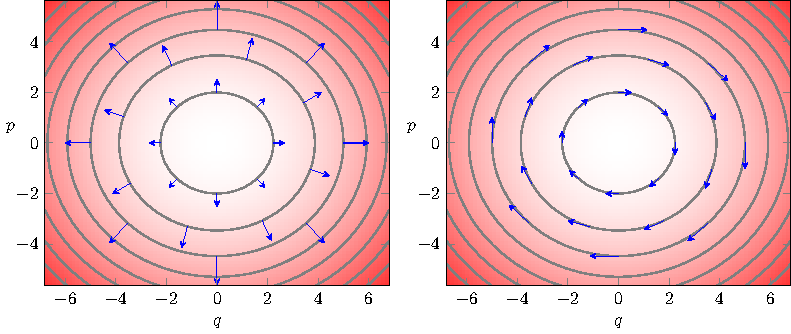
\includegraphics{images/fig_rp_cm_HamiltonianRotation.pdf}
	\caption {The surface plot shows the value of the Hamiltonian for a harmonic oscillator $H=\frac{p^2}{2m} + \frac{1}{2} k q^2$, red means higher value. The lines are the regions at constant energy $H$. On the left, the gradient of the Hamiltonian is shown. On the right, the displacement field is shown, which is the gradient rotated by a right angle. Note how the displacement is always parallel to the lines at constant energy.} \label{fig_rp_cm_HamiltonianRotation}
\end{figure}


We start by noting that the displacement field as expressed by \ref{rp-cm-hsd-displacementCurl} looks very similar to a curl of $H$, except that it is a two dimensional version. In vector calculus, a vector field is the curl of another field if and only if its divergence is zero.\footnote{We will leave for now topological requirements as they would be a distraction from the overall point.} This holds here as well. First, we can verify that
\begin{equation}
	\partial_a S^a = \partial_q S^q + \partial_p S^p = \partial_q \partial_p H - \partial_p \partial_q H = 0.
\end{equation}
Geometrically, this means that the flow of $S^a$ through a closed region is always zero. That is, $\oint \left( S^q dp - S^p dq \right) = 0$. Note that, since we are in a two dimensional space, a hyper-surface has dimension $n-1 = 2-1 = 1$ and therefore hyper-surfaces are lines. Therefore we have 
\begin{equation}
	\oint \left( S^q dp - S^p dq \right) = \oint \left( \partial_p H dp + \partial_q H dq \right) = \oint dH = 0.
\end{equation}
That is, the flow of the displacement field is the line integral of the gradient of $H$, which is zero over a closed curve.

Conversely, we can see that each divergenceless field in two dimensions admits a stream function $H$ that satisfies \ref{rp-cm-hsd-condEquations}. Geometrically, we can construct $H$ in the following way. Take a reference state $O$ in phase space and assign $H(O) = 0$. For any other state $P$, consider the flow of $S$ through any two lines that connect $O$ and $P$. Given that the flow through the region contoured by those lines must be zero, the flow through each line must be equal. Therefore the flow through a line that connects $O$ and $P$ only depends on the states, it is path independent. We can assign $H(P) = \int_{OP} \left( S^q dp - S^p dq \right)$. If we expand the differential of $H$ we have
\begin{equation}
	dH = \partial_q H dq + \partial_p H dp = - S^p dq + S^q dp.
\end{equation}
If we equate the components, we recover \ref{rp-cm-hsd-condEquations}. Geometrically, at least for the one dimensional case, we can understand the difference of the Hamiltonian between two states as the flow of the displacement field between them.

%\begin{figure}[h]
%	\centering
%	\begin{tikzpicture}
%	\end{tikzpicture}
%	\caption {TODO: F2 Difference of Hamiltonian is flow through line; Flow through region is always zero..}
%\end{figure}

We conclude that the following condition
\begin{equation}\label{rp-cm-hsd-condDivergenceDisplacement}
	\tag{DR-DIV}
	\eqtext{The displacement field is divergenceless: $\partial_a S^a = 0$} 
\end{equation}
is equivalent to \ref{rp-cm-hsd-condEquations}. Unlike \ref{rp-cm-hsd-condGeneralizedEquations}, this is a truly different mathematical condition.

Having looked at the flow through a region, we turn our attention to how regions themselves are transported by the evolution. Liouville's theorem states that volumes of phase space are preserved during Hamiltonian evolution, which in our case will be areas over the $q-p$ plane. To see this, let us review how variables transform, together with infinitesimal volumes:
\begin{equation}\label{rp-cm-volumeTransformation1d}
	\begin{aligned}
		\hat{\xi}^a &= \hat{\xi}^a(\xi^b) \\
		d\hat{\xi}^a &= \partial_b \hat{\xi}^a d\xi^b \\
		d\hat{\xi}^1 \cdots d\hat{\xi}^n &= \left| \partial_b \hat{\xi}^a \right| d\xi^1 \cdots d\xi^n \\
		d\hat{q} d\hat{p} &= \left|\begin{array}{ c c }
			\partial_q \hat{q} & \partial_p \hat{q} \\
			\partial_q \hat{p} & \partial_p \hat{p} \\
		\end{array} \right| dq dp \\
	\end{aligned}	
\end{equation}

This tells us that, mathematically, a transformation is volume preserving if the determinant of the Jacobian $\partial_b \hat{\xi}^a$ is unitary. If $\hat{q}$ and $\hat{p}$ represent the evolution of $q$ and $p$ after an infinitesimal time step $\delta t$, we have
\begin{equation}
	\begin{aligned}
	\hat{q} &= q + S^q \delta t \\ 
	\hat{p} &= p + S^p \delta t \\ 
	\partial_b \hat{\xi}^a &= \left[\begin{array}{ c c }
		1 + \partial_q S^q \delta t & \partial_p S^q \delta t \\
		\partial_q S^p \delta t & 1 + \partial_p S^p \delta t \\
	\end{array} \right] \\
	\left|\partial_b \hat{\xi}^a\right| &= (1 + \partial_q S^q \delta t) (1 + \partial_p S^p \delta t) - \partial_p S^q \, \partial_q S^p \, \delta t^2  = 1 + \left(\partial_q S^q + \partial_p S^p \right) \delta t + O(\delta t^2). 
	\end{aligned}
\end{equation}
Note that the first order term is proportional to the divergence of the displacement field, therefore the Jacobian determinant is equal to one if and only if the displacement is divergenceless. In other words, condition
\begin{equation}\label{rp-cm-hsd-condUnitaryJacobian}
	\tag{DR-JAC}
	\eqtext{The Jacobian of time evolution is unitary: $\left|\partial_b \hat{\xi}^a\right|=1$} 
\end{equation}
and condition
\begin{equation}\label{rp-cm-hsd-condConservedVolume}
	\tag{DR-VOL}
	\eqtext{Volumes are conserved through the evolution: $d\hat{\xi}^1 \cdots d\hat{\xi}^n = d\xi^1 \cdots d\xi^n$} 
\end{equation}
are equivalent to \ref{rp-cm-hsd-condDivergenceDisplacement}. We have found a third and a fourth way to characterize Hamiltonian evolution.

%\begin{figure}[h]
%	\centering
%	\begin{tikzpicture}
%	\end{tikzpicture}
%	\caption {TODO: F3 Conservations of areas and densities.}
%\end{figure}

While condition \ref{rp-cm-hsd-condConservedVolume} is expressed in terms of areas, similar considerations will work for densities because a density is a quantity divided by an infinitesimal area. In fact densities
\begin{equation}\label{rp-cm-densityTransformation1d}
	\begin{aligned}
		\left| \partial_b \hat{\xi}^a \right| \hat{\rho}(\hat{\xi}^a) &= \rho(\xi^b).
	\end{aligned}	
\end{equation}
transform in an equal and opposite way with respect to areas (i.e. the Jacobian determinant is on the other side of the equality). The unitarity of the Jacobian determinant, then, is equivalent to requiring that the density at an initial state is always equal to the density at the corresponding final state. Both areas and densities are transported unchanged by Hamiltonian evolution. Therefore
\begin{equation}\label{rp-cm-hsd-condConservedDensity}
	\tag{DR-DEN}
	\eqtext{Densities are conserved through the evolution: $\hat{\rho}(\hat{\xi}^a) = \rho(\xi^b)$ } 
\end{equation}
is yet another equivalent characterization.

To get a yet different perspective, we can reframe these arguments in terms of $\omega_{ab}$ and $S_a$. Given two vectors $v^a$ and $w^a$, the area of the parallelogram they form is $v^q w^p - v^p w^q$. This can be rewritten as $v^a \omega_{ab} w^b$, which means we can think of $\omega_{ab}$ as a tensor that, given two vectors, returns the area of the parallelogram they form.\footnote{More properly, $\omega_{ab}$ is a two-form.} If we denote $\hat{v}^a = \partial_b \hat{\xi}^a \, v^b$ and $\hat{w}^a = \partial_b \hat{\xi}^a \, w^b$ the transformed vectors, the invariance of the area can be written as
\begin{equation}
	v^a \omega_{ab} w^b = \hat{v}^c \omega_{cd} \hat{w}^d.
\end{equation}
Since
\begin{equation}
	\hat{v}^c \omega_{cd} \hat{w}^d = v^a \, \partial_a \hat{\xi}^c \omega_{cd} \, \partial_b \hat{\xi}^d \, w^b = v^a \, \hat{\omega}_{ab} w^b
\end{equation}
the previous equivalence means that $\omega_{ab} = \hat{\omega}_{ab}$, that is $\omega_{ab}$ remains unchanged. In other words, preserving the area for all possible pairs of vectors is the same as preserving the tensor $\omega_{ab}$ that returns the areas. We now see that $\omega_{ab}$ plays such an important geometric role that
\begin{equation}\label{rp-cm-hsd-condConservedSymplectic}
	\tag{DI-SYMP}
	\eqtext{The evolution leaves $\omega_{ab}$ invariant: $\hat{\omega}_{ab} = \omega_{ab}$} 
\end{equation}
is yet another equivalent characterization of Hamiltonian mechanics.

%\begin{figure}[h]
%	\centering
%	\begin{tikzpicture}
%	\end{tikzpicture}
%	\caption {TODO: F4 Areas from vectors.}
%\end{figure}

It is useful to look more closely at the definition of the Poisson bracket
\begin{equation}
	\{f, g\} = \partial_q f \, \partial_p g - \partial_p f \, \partial_q g = \left|\begin{array}{ c c }
		\partial_q f & \partial_p f \\
		\partial_q g & \partial_p g \\
	\end{array} \right|.
\end{equation}
For a single degree of freedom, the Poisson bracket coincides with the Jacobian determinant, where $f$ and $g$ are the two new variables. It essentially tells us how the volume changes if we change state variables from $[q, p]$ to $[f, g]$. Canonical transformations, then, are those that do not change the units of area. The Poisson bracket can be expressed\footnote{To see how our definitions and notation map to that used in differential geometry, let us define $\partial^a H = \omega^{ab} \partial_a H$. Note that $\partial^a H$ corresponds to the Hamiltonian vector field of $H$ usually noted $X_H$. The Poisson bracket is usually defined as $\omega(X_f, X_g)$. In our notation this becomes $\partial^a f \, \omega_{ab} \partial^b g = \omega^{ac} \partial_c f \omega_{ab} \omega^{bd} \partial_d g = \omega^{ac} \partial_c f \delta_a^d \partial_d g = \omega^{ac} \partial_c f \partial_a g$. One can see how the notation mimics the Einstein notation of general relativity and avoids the introduction of ad-hoc symbols.} as
\begin{equation}
	\{f, g\} = - \partial_a f \omega^{ab} \partial_b g = \partial_b g \omega^{ba} \partial_a f
\end{equation}
where 
\begin{equation}
	\omega^{ab} = \left[\begin{array}{cc}
		\omega^{qq} & \omega^{qp} \\
		\omega^{pq} & \omega^{pp} 
	\end{array} \right]= \left[\begin{array}{cc}
		0 & -1 \\
		1 & 0 
	\end{array} \right]
\end{equation}
is the inverse of $\omega_{ab}$. The invariance of the Poisson brackets is equivalent to the invariance of the inverse of $\omega_{ab}$, which is equivalent to \ref{rp-cm-hsd-condConservedSymplectic}. Therefore
\begin{equation}\label{rp-cm-hsd-condConservedPoisson}
	\tag{DI-POI}
	\eqtext{The evolution leaves the Poisson brackets invariant}
\end{equation}
is yet another equivalent characterization. So, again, we see how $\omega_{ab}$ plays a fundamental geometrical role.

We can also rewrite the flow of the displacement field
\begin{equation}
	\int \left( S^q dp - S^p dq \right) = \int S^a \omega_{ab} d\xi^b = \int S_b d\xi^b
\end{equation}
as the line integral of the rotated displacement field $S_a$. We can do that because in two dimensions the flow through a boundary is effectively a line integral along the boundary with the field rotated 90 degrees. This means that the following condition
\begin{equation}\label{rp-cm-hsd-condCurlRotatedDisplacement}
	\tag{DI-CURL}
	\eqtext{The rotated displacement field is curl free: $\partial_a S_b - \partial_b S_a = 0$} 
\end{equation}
is equivalent to condition \ref{rp-cm-hsd-condDivergenceDisplacement}.\footnote{Those familiar with relativistic electromagnetism will recognize the expression $\partial_a S_b - \partial_b S_a$ as the generalization of the curl. More properly, it is the exterior derivative applied to a one-form.} In fact, we can read equation \ref{rp-cm-hsd-condGeneralizedEquations} as saying that the rotated displacement field is the gradient of the scalar potential $H$.

We can see that we have found plenty of alternative characterizations of Hamilton's equations \ref{rp-cm-hsd-condEquations} (or \ref{rp-cm-hsd-condGeneralizedEquations}). Conditions  \ref{rp-cm-hsd-condDivergenceDisplacement}, \ref{rp-cm-hsd-condUnitaryJacobian}, \ref{rp-cm-hsd-condConservedVolume} and \ref{rp-cm-hsd-condConservedDensity} relate more directly to the displacement field $S^a$, while conditions \ref{rp-cm-hsd-condConservedSymplectic}, \ref{rp-cm-hsd-condConservedPoisson} and \ref{rp-cm-hsd-condCurlRotatedDisplacement} relate more directly to $\omega_{ab}$ and the rotated displacement field $S_a$. Nonetheless, they are all in terms of the mathematical description. While these are useful, the final goal of reverse physics is to find physical assumptions, not just equivalent mathematical definitions. So it is time to step back and try to understand what the math is really about.

\subsection{Physical characterizations}

Let us first reflect on what we just found out: the defining characteristic of Hamiltonian mechanics is not the transport of points, but the transport of areas and densities. If classical Hamiltonian mechanics were really about and only about point particles, there would be no reason for it to be characterized by \ref{rp-cm-hsd-condDivergenceDisplacement}, \ref{rp-cm-hsd-condConservedVolume} or \ref{rp-cm-hsd-condConservedDensity}. In fact, there would be no reason for the equations of motion \ref{rp-cm-hsd-condEquations} to be differentiable. Differentiable equations are exactly needed if we need to define the Jacobian, the transport of areas, or of densities defined on those areas. Classical point particles, then, are more aptly conceived not as points, but as infinitesimal regions of phase space, as distributions so peaked that only the mean value is important.

This, in retrospect, matches how classical mechanics is used in practice: planets, cannonballs, pendulums, beads on a wire, all the objects we study with classical mechanics are not point-like objects. They can be considered point-like if their size is negligible compared to the scale of the problem. If the distance between two celestial bodies is smaller than the sum of their radii, the point particle approximation clearly fails. This is also consistent with fluid dynamics and continuum mechanics, where we are literally studying the motion of infinitesimal parts of a material. It is interesting to see echoes of these considerations present in the mathematics.\footnote{We will want to investigate this link in more detail later.}

If we look at physics more broadly, we realize that in statistical mechanics we already have a physical interpretation for volumes of regions in phase space: they represent the number of states. Hamiltonian mechanics, then, maps regions while preserving the number of states. This means that, for each initial state there is one and only one final state, which leads to the following condition:
\begin{equation}\label{rp-cm-hsd-condDetRev}
	\tag{DR-EV}
	\eqtext{The evolution is deterministic and reversible.}	
\end{equation}
Note that by reversible here we mean that given the final state we can reconstruct the initial state. Given that areas measure the number of states, \ref{rp-cm-hsd-condDetRev} is equivalent to \ref{rp-cm-hsd-condConservedVolume}, which means this is another characterization of Hamiltonian mechanics. We can also see a connection to \ref{rp-cm-hsd-condConservedDensity}. If we assign a density to an initial state, and we claim that all and only the elements that start in that initial state will end in a particular final state, we will expect the density of the corresponding final state to match. That is, if the evolution is deterministic and reversible, it may shuffle around a distribution, but it will never be able to spread it or concentrate it.

This makes us understand, at a conceptual level, why a dissipative system, like a particle under linear drag, is not a Hamiltonian system. A dissipative system will have an attractor: a point or a region to which the system will tend given enough time. This means that, in time, the area around the attractor must shrink, the density will concentrate over the attractor, but this is exactly what Hamiltonian systems cannot do. Therefore Hamiltonian systems cannot have attractors, they cannot be dissipative. By the same argument, they can't have unstable points or regions from which the system always goes away.

What may be confusing is that the motion of a particle under linear drag may seem reversible, in the sense that we are able to, given the final position and momentum, reconstruct the initial values. Mathematically, it maps points one-to-one and would seem to satisfy \ref{rp-cm-hsd-condDetRev}, even though it is not a Hamiltonian system. This is a perfect example of how focusing on just the points leads to the wrong physical intuition. Physically, we would say that a one meter range of position allows for more configurations than a one centimeter range, even though mathematically they have the same number of points. If we understand that states are infinitesimal areas of phase space, we can see that a dissipative system, though it does map the center points of infinitesimal areas one-to-one, it does not map the full infinitesimal area one-to-one. In this sense dissipative systems fail to be reversible.

Let that sink in: we found that, if the system is deterministic and reversible, it admits a Hamiltonian, a notion of energy, and that energy is conserved over time. This may seem like a surprising and unexpected result. In retrospect, we can make an argument for it based on familiar physics considerations. If a system is deterministic and reversible it means that its evolution only depends on the state of the system itself. This means that it does not depend on the state of anything else. A system whose evolution does not depend on anything else is an isolated system. Therefore a deterministic and reversible system is isolated, and from thermodynamics we know that an isolated system conserves energy. It should not be surprising, then, that a deterministic and reversible system conserves energy. However, we found that not only does it conserve energy, it defines it. Therefore this link between mechanics and thermodynamics is actually deeper than we may think at first, and we should explore it further.

The idea that a dissipative system is not reversible sounds true on thermodynamic grounds. But thermodynamic reversibility is not the ability to reconstruct the initial state, but rather the existence of a process that can undo the change. Alternatively, a process is  thermodynamically reversible if it conserves thermodynamic entropy, which is a more precise characterization.\footnote{The actual existence of a reverse process is not something that can always be guaranteed.} We should not, then, confuse the two notions of reversibility, but we can easily show their relationship. The fundamental postulate of statistical mechanics tells us that the thermodynamic entropy $S = k_B \log W$ is the logarithm of the count of states, which corresponds to volume in phase space. Since the logarithm is a bijective function, conservation of areas of phase space is equivalent to conservation of entropy. Therefore
\begin{equation}\label{rp-cm-hsd-condThermoRev}
	\tag{DR-THER}
	\eqtext{The evolution is deterministic and thermodynamically reversible}	
\end{equation}
is yet another characterization of Hamiltonian mechanics.

There is another type of entropy that is also fundamental in both statistical mechanics and information theory: the Gibbs/Shannon entropy $I[\rho(\xi^a)]=-\int \rho \log \rho \, d\xi^1 \cdots d\xi^n$ which is defined for each distribution $\rho(\xi^a)$. Recalling the transformation rules for both volumes \ref{rp-cm-volumeTransformation1d} and densities \ref{rp-cm-densityTransformation1d}, we have
\begin{equation}
	\begin{aligned}
	I[\rho(\xi^a)] &= - \int \rho(\xi^a) \log \rho(\xi^a) \, d\xi^1 \cdots d\xi^n \\
&= - \int  \hat{\rho}(\hat{\xi}^b) \left| \partial_a \hat{\xi^b} \right| \log \left( \hat{\rho}(\hat{\xi}^b) \left| \partial_a \hat{\xi^b} \right| \right) \, d\xi^1 \cdots d\xi^n \\
&= - \int \hat{\rho}(\hat{\xi}^b) \log \left( \hat{\rho}(\hat{\xi}^b) \left| \partial_a \hat{\xi^b} \right| \right) \, d\hat{\xi}^1 \cdots d\hat{\xi}^n \\
&= - \int \hat{\rho}(\hat{\xi}^b) \log \hat{\rho}(\hat{\xi}^b) \, d\hat{\xi}^1 \cdots d\hat{\xi}^n - \int \hat{\rho}(\hat{\xi}^b) \log \left| \partial_a \hat{\xi^b} \right| \, d\hat{\xi}^1 \cdots d\hat{\xi}^n \\
&= I[\hat{\rho}(\hat{\xi}^b)] - \int \hat{\rho}(\hat{\xi}^b) \log \left| \partial_a \hat{\xi^b} \right| \, d\hat{\xi}^1 \cdots d\hat{\xi}^n.
	\end{aligned}
\end{equation}
Information entropy, then, remains constant if and only if the logarithm of the Jacobian determinant is zero, which means the Jacobian determinant is one. Therefore
\begin{equation}\label{rp-cm-hsd-condInformation}
	\tag{DR-INFO}
	\eqtext{The evolution conserves information entropy}	
\end{equation}
is equivalent to \ref{rp-cm-hsd-condUnitaryJacobian} and is yet another characterization of Hamiltonian mechanics.

The fact that determinism and reversibility is equivalent to conservation of information entropy should not be, in retrospect, surprising. Given a distribution, its information entropy quantifies the average amount of information needed to specify a particular element chosen according to that distribution. If the evolution is deterministic and reversible, giving the initial state is equivalent to giving the final state and therefore the information to describe one or the other must be the same. Determinism and reversibility, then, can be understood as the informational equivalence between past and future descriptions.

Lastly, given that entropy is often associated with uncertainty, it may be useful to understand how Hamiltonian evolution affects uncertainty. Given a multivariate distribution, the uncertainty is characterized by the covariance matrix
\begin{equation}
	cov(\xi^a, \xi^b) = \left[\begin{array}{ c c }
		\sigma^2_q & cov_{q, p} \\
		cov_{p, q} & \sigma^2_p \\
	\end{array} \right].
\end{equation}
The determinant of the covariance matrix gives us a coordinate independent quantity to characterize the uncertainty. If the distribution is narrow enough, we can use the linearized transformation to see how the uncertainty evolves after an infinitesimal time step $\delta t$. We have
\begin{equation}
	\left| cov(\hat{\xi}^c, \hat{\xi}^d) \right| = \left| \partial_a \hat{\xi}^c  \, cov(\xi^a, \xi^b) \, \partial_b \hat{\xi}^d  \right| = \left| \partial_a \hat{\xi}^c \right| \left| cov(\xi^a, \xi^b) \right| \left| \partial_b \hat{\xi}^d  \right|,
\end{equation}
which means the uncertainty remains unchanged if and only if the Jacobian is unitary. So
\begin{equation}\label{rp-cm-hsd-condUncertainty}
	\tag{DR-UNC}
	\eqtext{The evolution conserves the uncertainty of peaked distributions}	
\end{equation}
is equivalent to \ref{rp-cm-hsd-condUnitaryJacobian} and is another characterization of Hamiltonian mechanics.

%\begin{figure}[h]
%	\centering
%	\begin{tikzpicture}
%	\end{tikzpicture}
%	\caption {TODO: F5 Evolution of covariance matrix.}
%\end{figure}

This connection gives us yet another insight on the nature of determinism and reversibility in physics. Given that all physically meaningful descriptions are finite precision, a system is deterministic and reversible in a physically meaningful sense if and only if the past/future descriptions can be reconstructed/predicted at the same level of precision. This gives us another perspective as to why areas and densities must be conserved.

\subsection{Assumption of determinism and reversibility}

We have found twelve equivalent characterizations that link Hamiltonian mechanics, vector calculus, differential geometry, statistical mechanics, thermodynamics, information theory and plain statistics. Though we only talked about the case of a single degree of freedom, it gives us a much better idea of what systems Hamiltonian mechanics is supposed to describe, those that satisfy the following
\renewcommand{\theassump}{DR}
\begin{assump}[Determinism and Reversibility]\label{assum_detrev}
	The system undergoes deterministic and reversible evolution. That is, specifying the state of the system at a particular time is equivalent to specifying the state at a future (determinism) or past (reversibility) time.
\end{assump}
\renewcommand{\theassump}{\Roman{assump}}
We can see how this concept is implemented mathematically: it is not simply a one-to-one map between points. Classical particles should be more properly thought of as infinitesimal regions of phase space. Conceptually, the count of states, the thermodynamic entropy and information entropy are all conserved, and are all equivalent characterizations of determinism and reversibility. In terms of physical measurement, past and future states are given at the same level of uncertainty. But the most important lesson is that the foundations of classical mechanics are not disconnected from the foundations of all other disciplines we encountered. A full understanding of classical mechanics means understanding those connections as well.

\section{Multiple degrees of freedom}

We have seen how \ref{assum_detrev} is a constitutive assumption for Hamiltonian mechanics, and in fact is equivalent to Hamiltonian mechanics for one degree of freedom. We now turn our attention to the general case, and we will find that \ref{assum_detrev}, by itself, is not enough to recover the equations. We will need an additional assumption, that of the independence of degrees of freedom.

First, let's take Hamilton's equations for multiple degrees of freedom
\begin{equation}\label{rp-cm-hmd-condEquations}
	\tag{HM-ND}
	\begin{aligned}
		d_t q^i &= \partial_{p_i} H \\
		d_t p_i &= - \partial_{q^i} H
	\end{aligned}
\end{equation}
and re-express them in terms of generalized state variables. These will be noted as $\xi^a = [q^i, p_i]$ and will span a $2n$-dimensional space (i.e. manifold). The displacement field will be
\begin{equation}\label{rp-cm-displacementNd}
	S^a = d_t \xi^a = [d_t q^i, d_t p_i]
\end{equation}
which again is the vector field that defines the evolution of the system in time. Hamilton's equations, then, can be expressed as
\begin{equation}
	\begin{aligned}
		S^{q^i} &= \partial_{p_i} H \\
		S^{p_i} &= - \partial_{q^i} H.
	\end{aligned}
\end{equation}

Similarly to the previous case, let's introduce the following matrix
\begin{equation}\label{rp-cm-hmd-symplecticForm}
	\tag{SF-ND}
	\omega_{ab} = \left[\begin{array}{cc}
		\omega_{q^i q^j} & \omega_{q^i p_j} \\
		\omega_{p_i q^j} & \omega_{p_i p_j} 
	\end{array} \right]= \left[\begin{array}{cc}
		0 & I_n \\
		- I_n & 0 
	\end{array} \right] = \left[\begin{array}{cc}
	0 & 1 \\
	-1 & 0 
\end{array} \right] \otimes I_n
\end{equation}
which performs a 90 degree rotation within each degree of freedom, switching the components between position and momentum. That is, if $v^a = [v^{q^i}, v^{p_i}]$, then $v_a = v^b \omega_{ba}  = [-v^{p_i}, v^{q^i}]$.\footnote{For those versed in symplectic geometry, $v^a \omega_{ab}$ are the components of the one-form $\omega(v, \cdot)$. However, we are not going to call it a one-form as that assumes that the whole object is a map from a vector field to a scalar field, and we do not know whether that is the correct physical understanding. In other words, we want simply to understand what the quantities are doing without being tied, as much as possible, to a particular way to frame it. Full reverse engineering of differential geometry will be done in a later chapter, once the physics we need to describe is clear.} We can rewrite equation \ref{rp-cm-hmd-condEquations} as
\begin{equation}\label{rp-hm-HamiltonSymp}
	\begin{aligned}
		S_a = S^b \omega_{ba}  &= \partial_a H 
	\end{aligned}
\end{equation}
which notationally is the same as \ref{rp-cm-hsd-condGeneralizedEquations}. The insight that the displacement field is equal to the gradient of $H$ rotated 90 degrees still applies, except there are now multiple ways, in principle, to do that rotation. It is only the one defined by $\omega_{ab}$ that works.

Conditions \ref{rp-cm-hsd-condDivergenceDisplacement}, \ref{rp-cm-hsd-condUnitaryJacobian}, \ref{rp-cm-hsd-condConservedVolume} and \ref{rp-cm-hsd-condConservedDensity} are still satisfied and equivalent to each other. In fact, the divergence of the displacement field is zero
\begin{equation}
	\partial_a S^a = \partial_{q^i} S^{q^i} + \partial_{p_i} S^{p_i} = \partial_{q^i} \partial_{p_i} H - \partial_{p_i} \partial_{q^i} H = 0
\end{equation}
and the Jacobian is unitary
\begin{equation}
	\begin{aligned}
		\hat{q}^i &= q^i + S^{q^i} \delta t \\ 
		\hat{p}_i &= p_i + S^{p_i} \delta t \\ 
		\partial_{b} \hat{\xi}^a &= \left[\begin{array}{ c c }
			\delta_j^i + \partial_{q^j} S^{q^i} \delta t & \partial_{p_j} S^{q^i} \delta t \\
			\partial_{q^j} S^{p_i} \delta t & \delta_i^j + \partial_{p_j} S^{p_i} \delta t \\
		\end{array} \right] \\
		\left|\partial_{b} \hat{\xi}^a\right| &= \left|\delta_j^i + \partial_{q^j} S^{q^i} \delta t\right| \left|\delta_i^j + \partial_{p_j} S^{p_i} \delta t\right| - \left|\partial_{p_j} S^{q^i} \, \delta t \right| \, \left| \partial_{q^j} S^{p_i} \, \delta t \right| \\
		&= 1 + \left(\partial_{q^i} S^{q^i} + \partial_{p_i} S^{p_i} \right) \delta t + O(\delta t^2)
	\end{aligned}
\end{equation}
since the first-order term is again the divergence. The Jacobian is still the multiplicative factor between past/future areas (and densities), and therefore they are conserved even in the case of multiple degrees of freedom.

However, these conditions are not equivalent to \ref{rp-cm-hmd-condEquations}. The displacement field $S^a$ has $2n$ components and is therefore specified by $2n$ functions. Conditions \ref{rp-cm-hsd-condDivergenceDisplacement}, \ref{rp-cm-hsd-condUnitaryJacobian}, \ref{rp-cm-hsd-condConservedVolume} and \ref{rp-cm-hsd-condConservedDensity} specify the same single constraint, bringing down to $2n -1$ the number of independent components. The choice of Hamiltonian provides another constraint, leaving $2n - 2$ choices undetermined. In the single degree of freedom case, $n=1$, no choices are left, and therefore the displacement field is fully constrained. In the general case, however, this is not enough to fully characterize the evolution. Therefore \ref{rp-cm-hmd-condEquations} implies \ref{rp-cm-hsd-condDivergenceDisplacement}, \ref{rp-cm-hsd-condUnitaryJacobian}, \ref{rp-cm-hsd-condConservedVolume} and \ref{rp-cm-hsd-condConservedDensity}, but the converse is not true.

Let's see what happens to condition \ref{rp-cm-hsd-condConservedSymplectic}, the invariance of $\omega$ in the general case. We have
\begin{equation}
	\begin{aligned}
	\hat{\omega}_{ab} &= \partial_a \hat{\xi}^c \omega_{cd} \partial_b \hat{\xi}^d \\ &= \left(\delta_a^c + \partial_a S^c \delta t\right) \omega_{cd} \left(\delta_b^d + \partial_b S^d \delta t\right) \\
	&= \omega_{ab} + \left(\partial_a S^c \omega_{cb} + \omega_{ad} \partial_b S^d \right) \delta t + O(\delta t^2) \\
	&= \omega_{ab} + \left(\partial_a (S^c \omega_{cb}) + \partial_b ( S^d \omega_{ad}) \right) \delta t + O(\delta t^2) \\
	&= \omega_{ab} + \left(\partial_a (S^c \omega_{cb}) - \partial_b ( S^d \omega_{d a}  ) \right) \delta t + O(\delta t^2).
	\end{aligned}
\end{equation}
Therefore, the invariance of $\omega_{ab}$ is equivalent to
\begin{equation}
	\begin{aligned}
	\partial_a &(S^c \omega_{cb} ) - \partial_b (S^c \omega_{ca} ) = 0.
	\end{aligned}
\end{equation}
In terms of the rotated displacement field $S_a$ we have the more compact form
\begin{equation}
	\partial_a S_b - \partial_b S_a = 0.
\end{equation}
This tells us that the rotated displacement field $S_a$ is curl free, which is the same condition as \ref{rp-cm-hsd-condCurlRotatedDisplacement}, therefore \ref{rp-cm-hsd-condCurlRotatedDisplacement} and \ref{rp-cm-hsd-condConservedSymplectic} are equivalent conditions also in the general case.

Note that Hamilton's equations state that the rotated displacement field is the gradient of the Hamiltonian, and therefore
\begin{equation}
	\partial_a S_b - \partial_b S_a = \partial_a (S^c \omega_{cb}) - \partial_b (S^c \omega_{ca}) =  \partial_a \partial_b H - \partial_b \partial_a H = 0,
\end{equation}
which simply verifies that the curl of the gradient is zero. Conversely, if $S_a$ is curl-free, then it admits a scalar potential $H$ such that
\begin{equation}
	S_a = S^b \omega_{ba} = \partial_a H
\end{equation}
which recovers Hamilton's equations. Therefore \ref{rp-cm-hmd-condEquations}, \ref{rp-cm-hsd-condCurlRotatedDisplacement} and \ref{rp-cm-hsd-condConservedSymplectic} are equivalent.

The relationship between Poisson brackets and $\omega^{ab}$ is the same in the general case, therefore \ref{rp-cm-hsd-condConservedPoisson} and \ref{rp-cm-hsd-condConservedSymplectic} are equivalent as well.

To sum up, in the general case \ref{rp-cm-hmd-condEquations}, \ref{rp-cm-hsd-condGeneralizedEquations}, \ref{rp-cm-hsd-condConservedSymplectic}, \ref{rp-cm-hsd-condConservedPoisson} and \ref{rp-cm-hsd-condCurlRotatedDisplacement} are all equivalent and therefore full characterizations of Hamiltonian mechanics in the general case. These imply \ref{rp-cm-hsd-condDivergenceDisplacement}, \ref{rp-cm-hsd-condUnitaryJacobian}, \ref{rp-cm-hsd-condConservedVolume} and \ref{rp-cm-hsd-condConservedDensity}, which are all equivalent to one another, but weaker conditions that cannot recover Hamiltonian mechanics in full. For the second set of conditions, we already have an intuitive geometrical picture: the net flow of the displacement within a region of phase space is zero, volumes are preserved and so are densities. We need to build a stronger geometrical intuition for the first set, which is actually the more fundamental one.

Condition \ref{rp-cm-hsd-condConservedSymplectic} tells us that $v^a \omega_{ab} w^b$ is a conserved quantity, no matter what vectors $v^a$ and $w^b$ we choose. In the case of a single degree of freedom, this represented the area of the parallelogram formed by the two vectors, which was also the volume of the region. In the general case, we still have two vectors, but the situation is a bit more complicated.

We can gain an understanding by looking at the outer product decomposition for $\omega_{ab}$ we saw in \ref{rp-cm-hmd-symplecticForm}. This tells us that what happens within a degree of freedom is different from what happens across degrees of freedom. If we pick a single degree of freedom $1 \leq x \leq n$ and two vectors $v = v^q e_{q^x} + v^p e_{p_x}$ and $w = w^q e_{q^x} + w^p e_{p_x}$ that stretch along that degree of freedom, then we have
\begin{equation}
	v^a \omega_{ab} w^b =  v^q w^p - v^p w^q.
\end{equation}
That is, within each degree of freedom, $\omega_{ab}$ computes the area of the parallelogram. Since $\omega_{ab}$ is conserved, parallelograms within any degree of freedom will be mapped to parallelograms of the same size.

If we pick two different d.o.f. $x$ and $y$ and two corresponding vectors $v = v^q e_{q^x} + v^p e_{p_x}$ and $w = w^q e_{q^y} + w^p e_{p_y}$, then we have
\begin{equation}
	v^a \omega_{ab} w^b =  0.
\end{equation}
This defines a notion of orthogonality between different degrees of freedom. Since $\omega_{ab}$ is conserved, this notion of orthogonality is preserved during the evolution: orthogonal degrees of freedom are mapped to orthogonal degrees of freedom.

Those familiar with general relativity and/or Riemannian geometry may gain more insight by the following analogy. In those cases, the metric tensor $g_{ij}$ defines the geometry by defining the scalar product between vectors. That is, given two vectors $v^i$ and $w^j$, $v^i g_{ij} w^j = |v| |w| \cos \theta_{vw}$. Therefore the metric tensor defines the length and angles for vectors. In Cartesian coordinates, the metric tensor is a unitary matrix of the same dimension of the space. The form $\omega_{ab}$ does something in some sense similar and in some sense different. It defines areas within degrees of freedom and angles between them. Hamiltonian evolution preserves these areas and angles.

If areas and orthogonality are preserved, then volumes are preserved as well. The volume of a parallelepiped formed by parallelograms on orthogonal degrees of freedom will simply be the product of the areas of the parallelograms. Therefore we can understand why Hamiltonian mechanics satisfies \ref{rp-cm-hsd-condConservedVolume}. We can also understand why \ref{rp-cm-hsd-condConservedVolume} is not enough to recover Hamiltonian mechanics. An evolution could stretch one degree of freedom while shrinking another by the same amount. The total volume would remain the same, even though the area in each degree of freedom wouldn't. For example, take the system of equations:
\begin{equation}
	\begin{aligned}
	d_t q^1 &= S^{q^1} = \frac{p_1}{m} \\
	d_t p_1 &= S^{p_1} = - b p_1 \\
	d_t q^2 &= S^{q^2} = \frac{p_2}{m} \\
	d_t p_2 &= S^{p_2} = b p_2 \\
	\end{aligned}
\end{equation}
The first degree of freedom is a particle under linear drag, while the second is a particle accelerated (not decelerated) proportionally to its momentum by the same coefficient. We can verify that
\begin{equation}
	\partial_a S^a = \partial_{q^1} \frac{p_1}{m} + \partial_{p_1} (-b p_1) + \partial_{q^2} \frac{p_2}{m} + \partial_{p_2} (b p_2) = - b +b = 0
\end{equation}
the divergence is zero and therefore \ref{rp-cm-hsd-condDivergenceDisplacement} and \ref{rp-cm-hsd-condConservedVolume} are satisfied. However
\begin{equation}
	\partial_{q^1} S_{p_1} - \partial_{p_1} S_{q^1} = \partial_{q^1} S^{q^1} \omega_{q^1 p_1} - \partial_{p_1} S^{p_1} \omega_{p_1 q^1} = \partial_{q^1} \frac{p_1}{m} (1) - \partial_{p_1} (-b p_1) (-1) = -b.
\end{equation}
The curl of $S_a$, then, is not zero, \ref{rp-cm-hsd-condCurlRotatedDisplacement} is not satisfied, nor are \ref{rp-cm-hsd-condConservedSymplectic} and \ref{rp-cm-hmd-condEquations}. The system is not Hamiltonian precisely because we are not preserving the areas within each independent d.o.f.: the first is shrunk and the second stretched.

Now that we have a more precise understanding of the mathematics and the geometry, we should turn to the physics. Note that all the previous physical conditions \ref{rp-cm-hsd-condDetRev}, \ref{rp-cm-hsd-condThermoRev}, \ref{rp-cm-hsd-condInformation} and \ref{rp-cm-hsd-condUncertainty} are equivalent to \ref{rp-cm-hsd-condConservedVolume} and \ref{rp-cm-hsd-condUnitaryJacobian}. Therefore determinism and reversibility is clearly a constitutive assumption of Hamiltonian mechanics in the general case, but it cannot be the only one. Ideally, we would like to find a condition that is independent of \ref{assum_detrev}. However, we saw that \ref{rp-cm-hsd-condConservedSymplectic} implies \ref{rp-cm-hsd-condConservedVolume}, therefore the mathematics does not already give us two independent conditions we can map to the physics.

This is an important aspect to understand for reverse physics: the mapping between physical and mathematical conditions need not necessarily be one to one. A single mathematical condition can map to multiple physical ones, or the same physical condition can map to multiple mathematical ones. We saw before that determinism and reversibility forces the evolution map to be both bijective and volume preserving. Mathematically, these are two independent conditions. We can have a bijection that is not volume preserving (e.g. a linear transformation that stretches one side) or a volume preserving map that is not bijective (e.g. a map from $\mathbb{R}$ to $\mathbb{R}$ that maps all rationals to $0$ while leaving all the irrationals the same). Yet, a physically meaningful deterministic and reversible map must do both. Here we have the opposite: Hamiltonian mechanics implies determinism and reversibility, but is also implying at least another physical condition, and we need to understand which and whether it is physically independent.

Let's start from what we have already established: the phase space volume quantifies the number of states in the region. It stands to reason that the area on each degree of freedom identifies the number of configurations for that degree of freedom. Therefore, given two vectors, $v = v^q e_{q^x} + v^p e_{p_x}$ and $w = w^q e_{q^x} + w^p e_{p_x}$, constrained on a single degree of freedom $x$, the area of the parallelogram they identify, $v^q w^p - v^p w^q$, quantifies the number of configurations. Therefore $\omega_{ab}$ returns the number of configurations within each degree of freedom. What about between degrees of freedom?

As we saw, the conserved volume, which means the total number of states, is the product of those degrees of freedom that are orthogonal. In terms of $\omega_{ab}$, $x$ and $y$ are orthogonal if $\omega_{q^x q^y} = \omega_{q^x p_y} = \omega_{p_x q^y} = \omega_{p_x p_y} = 0$. In this case, the volume is simply the product of the phase space areas on the $x$ and $y$ degrees of freedom. This means that the total number of states is the product of the configurations of each degree of freedom. Physically, it means that a configuration choice for $x$ does not constrain the configurations for $y$. This means that the degrees of freedom are independent.

Given that there are different notions of independence, let us go through an example. Suppose we have a rabbit farm and describe its state with the number of males and females. These two variables are independent: if we say there are 231 females it doesn't, in principle, tell us anything about the number of males. Now, we may expect the population of both sexes to be about equal, and we may even find that in most rabbit farms that is the case, but this does not describe something about the nature of the variables themselves: it describes the nature of rabbit farms. Chicken farms, for example, would be predominantly females, as those are the ones that lay eggs.

Now we could choose to describe the rabbit farm with another set of variables: the number of females and the total number of rabbits. In this case, the variables are not independent. If we find that there are 231 females, it tells us, in principle, that there must be at least 231 rabbits. Conversely, if we find that there are 231 rabbits, there can only be up to 231 females. This dependence is not a feature of the rabbit farms. It does not just happen to be that there are no farms where the number of female rabbits exceeds the total number of rabbits. There can't be one.

This type of independence is very different from the notion of independence in terms of statistics and probability. The latter is in terms of whether the probability distribution factorizes. That is, if $P(f,m)$ is the probability that a particular rabbit farm has $f$ females and $m$ males, the distributions of males $P(m)$ and females $P(f)$ are independent if $P(f,m) = P(f) P(m)$. 

We therefore have two notions of independence. One is on the variables themselves and whether they can allow (i.e. whether we can measure) different combinations. One is on the probability distribution we may have in a particular case and whether it factorizes. The orthogonal directions in phase space, then, are independent in the first, stronger, sense. The degrees of freedom themselves are independent, regardless of what probability distribution one may put on top.

One may ask whether there is a link between the two, and in fact there is. Going back to our rabbits, we can easily see that, given any distribution $P(f)$ on the females, we can choose any distribution $P(m)$ on the males and set $P(f,m)=P(f)P(m)$. However, this does not happen for the total number. Suppose we chose $P(f)$ and we wanted to find a $P(f+m)$ such that $P(f, f+m) = P(f)P(f+m)$. The probability of the total number of rabbits could not change based on the number of females. If the probability of having 231 females is non-zero, then the probability of having less than 231 total rabbits in that case must be zero. But since we want the probability of having less than 231 rabbits independent of the number of females, then it must be zero for all cases. That is, the probability $P(f+m)$ must be zero for all numbers smaller than the greatest value of $f$ such that $P(f) \neq 0$. If there is no such greatest value of $f$, for example $f$ follows a geometric distribution, no $P(f+m)$ can exist that is independent of $P(f)$.

%[TODO: add a drawing showing that we are essentially trying to find a rectangular area on which to create the joint distribution. The diagonal constraint poses a problem. ]

The conclusion is that only independent variables can support independent distributions.\footnote{Formally, let $(\Omega, \mathcal{F}, P)$ be a probability space, let $X : \Omega \to E_X$ and $Y : \Omega \to E_Y$ be two random variables and $Z : \Omega \to E_X \times E_Y$ be their joint random variable (i.e. $Z(\omega) = (X(\omega), Y(\omega))$. Then $X$ and $Y$ are independent in this stronger sense if $Z(\Omega) = X(\Omega) \times Y(\Omega)$ and are statistically independent if the cumulative distribution function $F_Z(x,y)=F_X(x)F_Y(y)$ factorizes. Alternatively, they are independent if the $\sigma$-algebra generated by the joint distribution $Z$ is the product of the $\sigma$-algebras generated by $X$ and $Y$, and are statistically independent if the $\sigma$-algebras generated by $X$ and $Y$ are independent in the standard probability sense. } It should be clear that this observation is something that goes beyond the physical underpinning of Hamiltonian mechanics: it is something that applies to any variable to which we want to assign a probability distribution. As such, we do not want to expand the scope too much at this point, though clearly we will need to explore this more in full.

Here we limit ourselves to concluding that the following four conditions
\begin{align}
	\tag{IND-DOF}\label{rp-cm-hmd-condIndepDof}
	&\eqtext{The system is decomposable into independent DOFs} \\
	\tag{IND-STAT}\label{rp-cm-hmd-condIndepDistr}
	&\eqtext{The system allows statistically independent distributions over each DOF} \\
	\tag{IND-INFO}\label{rp-cm-hmd-condIndepEntropy}
	&\eqtext{The system allows informationally independent distributions over each DOF} \\
	\tag{IND-UNC}\label{rp-cm-hmd-condIndepUncertainty}
	&\eqtext{The system allows peaked distributions where the uncertainty is the product of the uncertainty on each DOF}
\end{align}
are equivalent. The first means that the count of states factorizes, the second that probability distributions can factorize, the third that the information entropy can sum, and the fourth that the determinant of the covariance matrix can factorize. Since only independent variables can support statistically independent distributions, \ref{rp-cm-hmd-condIndepDof} is equivalent to \ref{rp-cm-hmd-condIndepDistr}. Statistical independence of random variables coincides with independence of information entropy, therefore \ref{rp-cm-hmd-condIndepDistr} is equivalent to \ref{rp-cm-hmd-condIndepEntropy}. The uncertainty for peaked distributions factorizes if and only if the joint distribution is the product of independent distributions, therefore  \ref{rp-cm-hmd-condIndepDistr} is equivalent to \ref{rp-cm-hmd-condIndepUncertainty}.

Clearly these conditions are independent from \ref{assum_detrev}. We can imagine a deterministic and reversible system that cannot be broken into separate independent degrees of freedom, and we can imagine a system that can be broken into separate independent degrees of freedom that does not evolve deterministically or reversibly. The question is whether assuming independent degrees of freedom and deterministic and reversible evolution is enough to recover Hamiltonian mechanics. 

The first thing to check, then, is whether we have enough constraints to recover $\omega_{ab}$. Assuming that the system can be broken up into independent degrees of freedom, we must be able to define the count of configurations for each degree of freedom, and independent degrees of freedom must be orthogonal. The fact that $\omega_{ab}$ will return zero if it acts on directions belonging to independent degrees of freedom is really telling us that $\omega_{ab}$ counts not just configurations, but independent configurations. This, in retrospect, makes sense. But, so far this seems to restrict $\omega_{ab}$ to be
\begin{equation}
	\omega_{ab} = \left[\begin{array}{cc}
		0 & 1 \\
		-1 & 0 
	\end{array} \right] \otimes   \left[ {\begin{array}{cccc}
		a_{1} & 0 & \cdots & 0\\
		0 & a_{2} & \cdots & 0\\
		\vdots & \vdots & \ddots & \vdots\\
		0 & 0 & \cdots & a_{n}\\
\end{array} } \right].
\end{equation}
The fact that $\omega_{ab}$ must return the area in each degree of freedom constrains the left matrix of the outer product to the one above. The fact that $\omega_{ab}$ needs to return zero across independent degrees of freedom constrains the right matrix of the outer product to be diagonal. However, there is nothing, at this point, that seems to constrain the area of each d.o.f. to map to the same count of configurations. Naturally, we could simply rescale conjugate momentum in each d.o.f. to homogenize the count, but this would be an arbitrary freedom. Is there something forcing all the $a_i$ to be the same?

Note that $q^i$ and $p_i$ are not the only variables that form independent degrees of freedom. If we take two independent d.o.f. $x$ and $y$, $x+y$ and $x-y$ will also form independent degrees of freedom. That is, $\omega_{ab}$ defines orthogonality for all d.o.f., not just those of a particular basis. Changing $x$ and $y$ to $x+y$ and $x-y$ will effectively apply a rotation on the diagonal matrix, which will remain diagonal only if the coefficients on the diagonal are the same.

This tells us that if we want $\omega_{ab}$ to properly capture the independence of linear combinations of independent d.o.f., the diagonal matrix must have the same coefficient. This coefficient represents the freedom we have in choosing the units of omega with respect to the units of everything else. In SI units, by convention, the product between $q^i$ and $p_i$ is in $J\cdot s$ (i.e. the same units of $h$ and angular momentum) and we set the coefficient to 1. Therefore expressing the number of configurations with the same units for all d.o.f. is not an extra constraint, but it is necessary to keep track of the dependency relationship for all degrees of freedom.

Therefore the other constitutive assumption of Hamiltonian mechanics is
\renewcommand{\theassump}{IND}
\begin{assump}[Independent DOFs]\label{assum_indep}
	The system is decomposable into independent degrees of freedom. That is, the variables that describe the state can be divided into groups that have independent definition, units and count of states.
\end{assump}
\renewcommand{\theassump}{\Roman{assump}}
This assumption leads to conditions \ref{rp-cm-hmd-condIndepDof}, \ref{rp-cm-hmd-condIndepDistr}, \ref{rp-cm-hmd-condIndepEntropy} and
\ref{rp-cm-hmd-condIndepUncertainty}, which we saw implies the existence of a form $\omega_{ab}$ that defines the independence of d.o.f. together with the count of independent configurations for each d.o.f.. Conversely, assuming \ref{rp-cm-hmd-condEquations} means defining an $\omega_{ab}$ such that \ref{assum_indep} is satisfied. The last question is whether \ref{assum_detrev} and \ref{assum_indep} are enough to recover \ref{rp-cm-hmd-condEquations}.

As we saw, \ref{assum_indep} by itself means the existence of the counting form $\omega_{ab}$. Meanwhile, \ref{assum_detrev} by itself means the conservation of the total number of states, the volume. These two mathematical conditions, by themselves, do not lead to Hamiltonian mechanics. We need that the counting form itself is conserved, meaning that d.o.f. independence and the configuration count is preserved. This boils down to the following question: does it make sense, on physical grounds, to have a deterministic and reversible evolution that takes a system decomposable into independent degrees of freedom and turns it into a system that is no longer decomposable? More specifically, can deterministic and reversible evolution take two independent degrees of freedom and break their independence?

We should remind ourselves that independence here is not statistical independence. Clearly, Hamiltonian evolution can add correlations, and therefore evolve the product of two independent distributions into something that is no longer factorizable. This is not the question at hand. The notion of independence on the table is the one that tells us that all the combinations of configurations are at least possible. Recall the example of the rabbits: number of females and total rabbits are not independent because we cannot have more females than rabbits. This is the type of independence we are interested in. Can deterministic and reversible evolution lose this type of independence?

The answer is, as you may expect, no. This is easily seen in the finite case. Suppose we have two integer variables, $1 \leq x \leq 3$ and $1 \leq y \leq 3$. If they are independent, we have a total of $9$ distinct cases. If the evolution is deterministic and reversible, we will still have $9$ distinct cases, which means the variables must remain independent. Note that we may introduce a correlation between $x$ and $y$. But still, we need $9$ total cases.

The issue here is that the case of independent variables is maximal as it posits that all combinations of configurations are possible. Therefore, the only way to make variables no longer independent is to decrease the number of distinct cases, which cannot happen during deterministic and reversible evolution. The same must happen in the infinite or the continuous case, because finite ranges must still be comparable with finite sizes which must hold the same property. Therefore when we take both physical assumptions \ref{assum_indep} and \ref{assum_detrev}, the physics tells us that independence of degrees of freedom must be preserved, which means preserving $\omega_{ab}$ as well. In other words:
\begin{insight}
	Hamiltonian mechanics is exactly the deterministic and reversible evolution of a system decomposable into a finite collection of independent degrees of freedom.
\end{insight} 

This conclusion is yet another example of why just looking at the math is not enough. Two physical conditions taken separately may each impose one mathematical condition, but it is not necessarily true that imposing them together will only impose the conjunction of the two mathematical conditions. More than a problem with math in general, we believe it is an indication that the math we currently use is not the ``physically correct'' one as it does not seem to be capturing the entirety of the physical conditions. 

Note that, in principle, we could ask the evolution to preserve the independence of d.o.f. without requiring \ref{assum_detrev}. As we saw, fixing all independent d.o.f. fixes $\omega_{ab}$ up to a scalar factor, which could change during the evolution. The volume would stretch or shrink depending on the factor, stretching or shrinking each d.o.f. by the same amount. An example of this would be a particle under linear drag in three dimensions. Since a faster moving object will be subjected to a greater frictional force, a spread in momentum $\Delta p$ will become smaller in time, and will tend to zero as time increases. Given that the friction coefficient is the same for all directions, all degrees of freedom will shrink at the same rate. If we understand the volume as entropy, this tells us that the only way we can add or remove entropy to/from a system while preserving the independence of the degrees of freedom is by dividing that entropy contribution equally among each d.o.f.. In other words, preservation of d.o.f. independence gives us a sort of equipartition of entropy change. It is again striking to find these connections between disciplines at such a basic level.

To conclude, we now have a mathematically and physically precise way to characterize Hamiltonian evolution. We had found that Hamiltonian mechanics did not apply to all cases, and now we know exactly to which cases it applies: systems described by finitely many independent degrees of freedom undergoing deterministic and reversible evolution.

\section{Reversing differential topology}

In the previous sections, we saw that elements of differential topology and differential geometry started appearing: we employed a generalization of the curl and we used the form $\omega_{ab}$ to lower indexes, much like one does in general relativity with the metric tensor $g_{\alpha\beta}$. Since we will use these tools more and more, we should take a detour and understand the physical significance of the tools themselves. We will end up with a generalized notion of integral and of differential operations that work with an arbitrary number of dimensions. We will also conclude that to reach the full potential of reverse physics, we need to apply the same techniques not just to the equations themselves, but to the mathematical tools we use to formulate them.

% Final TODO: decide between phase space or phase-space

The main reason we are forced to abandon vector calculus in favor of differential topology and geometry is that vector calculus works in three dimensions but does not generalize to an arbitrary dimensional space. Special and general relativity, for example, live on a four-dimensional space-time; Hamiltonian and Lagrangian mechanics live in phase-space, which can have an arbitrarily large number of degrees of freedom. Similarly to what we have done with the equations, we will start from the expressions of vector calculus, see their limitations, and construct generalized ones. We warn the reader who is already familiar with differential topology that this process will give us notation and concepts that are slightly different from what is used by mathematicians. We will discuss these differences at the end of the section.

The first tool we need to generalize is that of line, surface and volume integrals. For example, the mass $m$ within a region $V$ can be understood as the sum of the contributions of a mass density $\rho$ within each infinitesimal volume $dV$:
\begin{equation}
	m(V) = \iiint_V \rho dV.
\end{equation}
Similarly, the magnetic flux $\Phi$ through a surface $\Sigma$ can be understood as the sum of the contributions of the magnetic field $\vec{B}$ over each infinitesimal $d\vec{\Sigma}$:
\begin{equation}
	\Phi(\Sigma) = \iint_\Sigma \vec{B} \cdot d\vec{\Sigma}.
\end{equation}
Lastly, the work $W$ over a path $\gamma$ can be understood as the sum of the contributions of a force field $\vec{f}$ over each infinitesimal segment $d\vec{\gamma}$:
\begin{equation}
	W(\gamma) = \int_\gamma \vec{f} \cdot d\vec{\gamma}.
\end{equation}

Note the pattern: the functionals $W$, $\Phi$ and $m$ all take a region of space while $\vec{f}$, $\vec{B}$ and $\rho$ act on infinitesimal regions. However the pattern is not completely consistent. In the line integral case, we have the product between a vector representing the force and a vector representing the displacement along the line. In the surface integral case we have the product between a pseudo-vector representing the magnetic force and a pseudo-vector representing the normal to the surface element. In the volume integral case we have the product between a pseudo-scalar representing the density and a pseudo-scalar representing the volume of the infinitesimal region. Each operation is slightly ad-hoc. Moreover, a surface has a single perpendicular direction only in three dimensions. In four dimensions, for example, there are multiple different perpendiculars to the same plane. Lastly, they all require a notion of product between vectors, an inner product, which in differential geometry is only defined on Riemannian spaces, those that define a metric tensor. That is, those spaces in which angles and distances are well defined. In physics we are so used to working with spaces that have an inner product that it may seem that all spaces provide one, but that is not the case. In phase space, there is no way to compare differences in position with differences in momentum, therefore we do not have a metric to take a scalar product; there is no overall notion of distance and angle. In general, if we imagine the space that represents all possible outcomes of a blood test, this will form a manifold as each test can be fully described by a finite set of continuous quantities. In this space, there is no natural notion of distance and angles between directions, there is no notion of geometry. As we will see, the notion of integral, the idea of a quantity that can be understood as the sum of infinitely many infinitesimally small contributions, does not require either a particular number of dimensions or a notion of distance and angle.

Suppose we understood $\vec{f}$, $\vec{B}$ and $\rho$ not as above, but as maps that for each infinitesimal region return an infinitesimal contribution $dW$, $d\Phi$ and $dm$. We could simply write
\begin{equation*}
	\begin{aligned}
		W(\gamma) &= \int_\gamma dW = \int_\gamma f(d\gamma) \\
		\Phi(\Sigma) &= \iint_\Sigma d\Phi = \iint_\Sigma B(d\Sigma) \\
		m(V) &= \iiint_V dm = \iiint_V \rho(dV).
	\end{aligned}
\end{equation*}
This pattern is straightforward and more easily generalized. We call these functions of infinitesimal regions $k$-forms, where $k$ is the dimensionality of the infinitesimal region they take as an argument. The force, in this notation, is a one-form (or covector) as it takes one dimensional infinitesimal regions (i.e. vectors); the magnetic field is a two-form; the density is a three-form. We can also say that a scalar field, like the temperature, is a zero-form, as it takes points, zero dimensional objects.

Since $k$-forms act over infinitesimal regions, they will have some key properties.  First, note that each infinitesimal region can be understood as a parallelepiped, and a parallelepiped is fully identified by its sides. Therefore, a $k$-form can be understood as acting on a set of infinitesimal displacements, the sides of the parallelepiped, whose number matches the dimensionality of the form. A one-form will take one displacement, a two-form two displacements and so on. Second, as they are linear functions of the infinitesimal regions, they will also be linear functions of the vectors that define these infinitesimal regions. Lastly, all forms must be anti-symmetric because switching the order of the sides does not change the parallelepiped, but it changes its orientation.

We can write displacements and forms in terms of components and basis elements
\begin{equation}
	\begin{aligned}
	dP &= dx^i e_i \\
		f &= f_i e^i \\
		B &= B_{ij} e^i \otimes e^j \\
		\rho &= \rho_{ijk} e^i \otimes e^j \otimes e^k.
	\end{aligned}
\end{equation}
The anti-symmetry means that switching the indexes introduces a minus sing. For example, $B_{ij} = - B_{ji}$ and $\rho_{ijk} = - \rho_{jik}$. Therefore, our integrals can be written as
\begin{equation}
	\begin{aligned}
		W(\gamma) &= \int_\gamma f_i \, dx^i \\
		\Phi(\Sigma) &= \iint_\Sigma B_{ij} \, dx_1^i \, dx_2^j \\
		m(V) &= \iiint_V \rho_{ijk} \, dx_1^i \, dx_2^j \, dx_3^k.
	\end{aligned}
\end{equation}
Each $k$-form, then, is a fully anti-symmetric covariant tensor, with one index for each dimension of the form. In this view, the $B^x$ component of the magnetic field, then, becomes the $B_{yz}$ component. That is, instead of being the component that gives us the magnetic flux along the $x$ direction, it is the component that gives us the flux through the $yz$ plane. Similarly, $\rho_{xyz}$ is better understood not as the value of the mass density at a point, but rather the value of the density over the $xyz$ volume. The indexes make unit dependency apparent as well: $B_{yz}$ must be in units of magnetic flux divided by the units of $y$ and $z$; $\rho_{xyz}$ must be in units of mass divided by the units of $x$, $y$ and $z$; in spherical coordinates, $B_{r\theta}$ must be in units of magnetic flux divided by units of $r$ and $\theta$. In fact, one can argue that these tools are here exactly to keep track of the units of the components.

We can go further, and rewrite the integrals in terms of parametrizations of the surfaces and the components of the forms along said parametrization. We have
\begin{equation}
	\begin{aligned}
		W(\gamma) &= \int_\gamma f_i dx^i = \int_{a_u}^{b_u} f_i \partial_u x^i du = \int_{a_u}^{b_u} f_u du \\
		\Phi(\Sigma) &= \iint_\Sigma B_{ij} \, dx_1^i \, dx_2^j = \int_{a_u}^{b_u} \int_{a_v}^{b_v} B_{ij} \, \partial_u x_1^i du \, \partial_v x_2^j dv = \int_{a_u}^{b_u} \int_{a_v}^{b_v} B_{uv} du dv \\
		m(V) &= \iiint_V \rho_{ijk} \, dx_1^i \, dx_2^j \, dx_3^k = \int_{a_u}^{b_u} \int_{a_v}^{b_v} \int_{a_w}^{b_w} \rho_{ijk} \,  \partial_u x_1^i du \, \partial_v x_2^j dv \, \partial_w x_3^k dw \\
		&= \int_{a_u}^{b_u} \int_{a_v}^{b_v} \int_{a_w}^{b_w} \rho_{uvw} du dv dw.
	\end{aligned}
\end{equation}
These expressions are useful to write the integrals in terms of an integral of $k$ variables. This is particularly useful if the surfaces possess different symmetries than the forms, which allows one to use the parametrization appropriately.

We now have expressions that are easier to generalize. If we denote $S^k$ the space of all the $k$-dimensional subregions of an $n$-dimensional manifold, a $k$-functional $F_k : S^k \to \mathbb{R}$ is an additive functional that takes a $k$-surface $\sigma^k$ and returns a number. This can be expressed as
\begin{equation}
	\begin{aligned}
		F_k(\sigma^k) &= \int_{\sigma^k} \omega_k (d\sigma^k) = \int_{\sigma^k} \omega_{i_1 i_2 \cdots i_k} \, dx_1^{i_1} \, dx_2^{i_2} \, \cdots \, dx_k^{i_k} \\
		&= \int_{a_{u_1}}^{b_{u_1}} \int_{a_{u_2}}^{b_{u_2}} \cdots \int_{a_{u_k}}^{b_{u_k}} \omega_{u_1 u_2 \cdots u_k} \, du_1 \, du_2 \, \cdots \, du_k,
	\end{aligned}
\end{equation}
which is the integral of a $k$-form $\omega_k : V^k \to \mathbb{R}$. Here $V$ is the space of vectors, of infinitesimal displacements, and an infinitesimal $k$-surface $d\sigma^k$ is defined by an ordered set of $k$ vectors, therefore is an element from the Cartesian product $V^k = V \times V \times \cdots \times V$. The $k$-form takes an infinitesimal $k$-surface $d\sigma^k$ and returns a number. We now have a way to express local objects and integrals in a generalized way.

% Final TODO: V is volume and V is the space of vectors

In the spirit of reverse physics, we ask: what are the physical assumptions that are required to use these mathematical objects? Note that we do not measure mass density $\rho$ directly: we measure mass $m$ within a finite region $V$ and the size of the finite region $V$, and we calculate the mass density by dividing the first by the second. The mass density $\rho$  is the limit for which the region $V$ shrinks to a point.\footnote{This is essentially the definition of the Radon-Nikodym derivative used in measure theory.} The same happens with the other quantities. We do not measure a force $f$ directly, but rather the work that a force performs, for example, by deforming a spring. In other words, we measure the finite value of the functional $F$ over a finite region $\sigma$, and the form $\omega$ returns the limit of $F$ for infinitesimal regions. Note that it is crucial for $F$ to be additive, that is, if $\sigma_1$ and $\sigma_2$ are two disjoint regions, $F(\sigma_1 \cup \sigma_2) = F(\sigma_1) + F(\sigma_2)$. Physically, it means that the contribution of one sub-region is independent from the other, because if this isn't the case, we cannot assign a unique value to each region. While this may seem a relatively harmless assumption, it may not hold in general. For example, suppose we have a system distributed in space. Given the mass-energy equivalence, the mass is an additive functional only if the interaction between the parts can be neglected. In fact, if the interaction energy at the boundary is so large that it is of the same scale of the mass within the regions, then it is not true that the total mass is simply the mass within each region. Therefore, if we write the mass density $\rho$, we have implicitly assumed that the interaction energy between parts can be neglected. While this is going to be true in a large number of cases, it is something we have to keep in mind. The functional $F$, in fact, is a more general physical object as it may exist even though infinitesimal additivity fails.

If the functional $F$ respects the limits, in the sense that small variations of the region result in small variations of the value of the functional, then we can express the functional $F$ as the integral of a form $\omega$.\footnote{Mathematically, one needs to be precise as to what these small variations are, and what the space of regions is. Effectively, we need to define what it means for $k$-surfaces to be differentiable. This is more in the scope of physical mathematics than reverse physics.} Note that the standard mathematical definitions are inverted with respect to what makes physical sense. Mathematically, we first define the form and then its integration, and we may worry whether the integral exists or diverges; physically, we first define the functional of finite regions and worry about the existence of an infinitesimal limit, the form, under additional physical assumptions. This is important because, as we said before, it tells us that it is the functional that survives when the assumption fails, not the form. It also means that, if we want to get a robust physical intuition, we should concentrate on the functionals, the finite objects, rather than the forms, the infinitesimal objects.

%TODO: transform into insight
We would be tempted to conclude something along the lines of
\begin{equation}
	\eqtext{Differential $k$-forms represent the infinitesimal contributions of an infinitesimally additive quantity $F_k$ that depends on a $k$-dimensional surface.}
\end{equation} 
The issue here is that while we have a sense that, mutatis mutandi, an infinitesimally additive functional corresponds to a differential form, we would need to show that differential forms cannot represent anything else. We currently do not have such an argument, though we suspect it should exist. One may first note that no measurement can really be conducted at a point, and therefore it has to extend, at least in principle, over a $k$-dimensional region. Therefore we could argue that all measurements are functionals, additive or not. This means that we would need a map between the value of the components of the form at all points and the value of the functional over all regions. To reach our goal, we would need to show that this map can be established only if the functional is infinitesimally additive, which may not be a strong enough condition by itself. While we are already implicitly assuming the map to be differentiable, we could impose further requirements on the measurement functional. We could impose locality, in the sense that changes of the form within a region must change the value of the functional for said region; it would also mean that changes outside of the region do not affect measurements in the region. While we do not know whether these requirements are sufficient, these are the types of questions we would need to answer in order to have a fully physically meaningful treatment of differential forms.

Having generalized the idea of integration, let us now turn to differential operators such as gradient, curl and divergence. Suppose that $T$ is a scalar field, like the temperature. Then we have the following relationship
\begin{equation}\label{rp-cm-dg-gradientTheorem}
	\int_{\gamma} \vec{\nabla} T \cdot d\vec{\gamma} = T(B) - T(A).
\end{equation}
That is, the integral of the gradient of $T$ along $\gamma$ gives us the difference of $T$ evaluated at the endpoints, the boundary of the line. If $\vec{f}$ is a vector field, like the force, we have
\begin{equation}\label{rp-cm-dg-curlTheorem}
	\iint_{\Sigma} \vec{\nabla} \times \vec{f} \cdot d\vec{\Sigma} = \int_{\gamma = \partial \Sigma} \vec{f} \cdot d\vec{\gamma} = W(\gamma)
\end{equation}
That is, the integral of the curl of $\vec{f}$ over a surface $\Sigma$ is equal to the line integral of $\vec{f}$ over the boundary. If $\vec{B}$ is a pseudo-vector field, like the magnetic field, we have
\begin{equation}\label{rp-cm-dg-divergenceTheorem}
	\iiint_{V} \vec{\nabla} \cdot \vec{B} \, dV = \iint_{\Sigma = \partial V} \vec{B} \cdot d\vec{\Sigma} = \Phi(\Sigma).
\end{equation}
That is, the integral of the divergence of $\vec{B}$ over a region $V$ is equal to the surface integral of $\vec{B}$ over the boundary. Note the pattern: the integral of the differential operator applied to the bulk becomes the integral of the original object over the boundary.

Let us understand how this works in terms of functionals. Given the temperature $T(P)$, we can construct a line functional that for each line returns the difference in temperature at the endpoints. Given the work line functional $W(\gamma)$, we can construct a surface functional that for each surface returns the work needed to go around the contour. Given the magnetic flux surface functional $\Phi(\Sigma)$, we can construct a volume functional that for each volume returns the magnetic flux over the boundary. In general, suppose we have a $k$-functional $F_k : S^k \to \mathbb{R}$. To each $k$-surface $\sigma^k$ we can associate a quantity $F_k(\sigma^k)$. Now, suppose we are given a $(k+1)$-surface $\sigma^{k+1}$. While $F_k$ cannot act on $\sigma^{k+1}$, the boundary $\partial \sigma^{k+1}$ is a $k$-surface, therefore we can evaluate $F_k(\partial \sigma^{k+1})$. Therefore, we can define the $(k+1)$-functional $\partial F_k$ such that $\partial F_k (\sigma^{k+1}) \mapsto F_k(\partial \sigma^{k+1})$, which we call the exterior functional of $F_k$.\footnote{Mathematically, we would have to prove that $\partial F_k$ is a functional. Again, these mathematical details are left for the physical mathematics section. For now, we are more interested in the conceptual understanding.} Since the exterior functional is an additive functional, it will have a corresponding form that acts on the infinitesimal region. Conceptually, the gradient of $T$ is the one-form that corresponds to the boundary functional of $T$; the curl of $\vec{f}$ is the two-form that corresponds to the boundary functional of the work $W$, the line integral of $\vec{f}$; the divergence of $\vec{B}$ is the three-form that corresponds to the boundary functional of the magnetic flux $\Phi$, the surface integral of $\vec{B}$. The problem is, again, that the gradient, curl and divergence are not expressed in a way that is easy to generalize.

Given that all three operators are in terms of $\nabla$, which in components is written $\partial_i$, we would like to write something along the lines of 
\begin{equation}\label{rp-cm-dg-generalizedStokes}
	\begin{aligned}
		\partial F_k(\sigma^{k+1}) &=\int_{\sigma^{k+1}} \partial_{i_0} \wedge \omega_{i_1 i_2 \cdots i_k} dx^{i_0} dx^{i_1} dx^{i_2} \cdots dx^{i_k} \\
		&= \int_{\partial \sigma^{k+1}} \omega_{i_1 i_2 \cdots i_k} dx^{i_1} dx^{i_2} \cdots dx^{i_k} = F_k(\partial \sigma^{k+1}).
	\end{aligned}
\end{equation}
The operation $\wedge$, which we call exterior product, must be such that we recover something consistent to the previous operations. That is, we need
\begin{equation}
	\begin{aligned}
		\partial_i \wedge T &= \partial_i T \\
		\partial_i \wedge F_j &= \partial_i F_j - \partial_j F_i \\
		\partial_i \wedge B_{jk} &= \partial_{i} B_{jk} + \partial_{j} B_{ki} + \partial_{k} B_{ij} 
	\end{aligned}
\end{equation}
These would be the expressions we need to recover the gradient, curl and divergence respectively. Let us study them to see the pattern. Fist of all, each expression takes a $k$-form and returns a $(k+1)$-form by adding a derivation along each index. Given that we have a derivation for each index, the number of terms matches the number of indexes of the final form, which is $k+1$. Each term changes index by taking a cyclic permutation. Recall that the forms are anti-symmetric, therefore each permutation of two indexes introduces a minus sign. A cyclic permutation of $k+1$ elements corresponds to $k$ pair swaps. If $k+1$ is odd, then, each cyclic permutation will correspond to an even number of sign switches, which cancel out. The pattern, then, generalizes in the following way
\begin{equation}
	\begin{aligned}
		\partial_{i_0} \wedge \omega_{i_1 i_2 \cdots i_k} &= \partial_{i_0} \omega_{i_1 i_2 \cdots i_k} + (-1)^{k} \partial_{i_1} \omega_{i_2 \cdots i_k i_0} + (-1)^{2\cdot k} \partial_{i_2} \omega_{i_3 \cdots i_k i_0 i_1} + \cdots \\
		&+ (-1)^{k\cdot k} \partial_{i_k} \omega_{i_0 i_1 \cdots i_{k-1}} \\
		&= \sum_{j=0}^{k} (-1)^{j\cdot k} \partial_{i_{j \bmod k+1}} \omega_{i_{j+1 \bmod k+1} i_{j+2 \bmod k+1} \cdots i_{j+k \bmod k+1}}.
	\end{aligned}
\end{equation}
The use of $\mod k+1$ in the generalized expression makes sure that the index jumps from $i_k$ to $i_0$. This gives us a fully anti-symmetric tensor which matches the gradient, curl and divergence in the simple cases.\footnote{In principle, we could write the expression in different equivalent ways. Here we used cyclic permutations as it gives a more elegant expression.} This operation is called the exterior derivative.

While we have the expression for the exterior derivative, we would like to understand why and how the expression works. Geometrically, we can imagine integrating along a parallelepiped, which becomes
\begingroup
\allowdisplaybreaks
\begin{align*}
		\int_{\sigma^{k+1}} (\partial \wedge \omega_k) (d\sigma^{k+1}) &= \int_{\sigma^{k+1}} \partial_{i_0} \wedge \omega_{i_1 i_2 \cdots i_k} \, dx_0^{i_0} \, dx_1^{i_1} \, \cdots \, dx_k^{i_k} \\
		&= \int_{a_{u_0}}^{b_{u_0}} \int_{a_{u_1}}^{b_{u_1}} \cdots \int_{a_{u_k}}^{b_{u_k}} (\partial_{u_0} \omega_{u_1 u_2 \cdots u_k} + (-1)^{k} \partial_{u_1} \omega_{u_2 \cdots u_k u_0} \\
		&+ \cdots 
		+ (-1)^{k \cdot k} \partial_{u_k} \omega_{u_0 u_1 \cdots u_{k-1}} )du_0 \,du_1 \, du_2 \, \cdots \, du_k \\
		&= \int_{a_{u_1}}^{b_{u_1}} \cdots \int_{a_{u_k}}^{b_{u_k}} \int_{a_{u_0}}^{b_{u_0}} du_0 \partial_{u_0} \omega_{u_1 u_2 \cdots u_k} \,du_1 \, du_2 \, \cdots \, du_k \\
		&+ (-1)^{k} \int_{a_{u_0}}^{b_{u_0}} \int_{a_{u_2}}^{b_{u_2}} \cdots \int_{a_{u_k}}^{b_{u_k}} \int_{a_{u_1}}^{b_{u_1}} du_1 \partial_{u_1}  \omega_{u_2 \cdots u_k u_0} \,du_0 \, du_2 \, \cdots \, du_k \\
		&+ \cdots + (-1)^{k \cdot k} \int_{a_{u_0}}^{b_{u_0}} \int_{a_{u_1}}^{b_{u_1}} \cdots \int_{a_{u_{k}}}^{b_{u_k}} du_k  \partial_{u_k} \omega_{u_0 u_1 \cdots u_{k-1}} \,du_0 \, du_1 \, \cdots \, du_{k-1} \\
		&= \left[ \int_{a_{u_1}}^{b_{u_1}} \cdots \int_{a_{u_k}}^{b_{u_k}} \omega_{u_1 u_2 \cdots u_k} \,du_1 \, du_2 \, \cdots \, du_k \right]_{a_{u_0}}^{b_{u_0}} \\
		&+ (-1)^{k} \left[ \int_{a_{u_0}}^{b_{u_0}} \int_{a_{u_2}}^{b_{u_2}} \cdots \int_{a_{u_k}}^{b_{u_k}}\omega_{u_2 \cdots u_k u_0} \,du_0 \, du_2 \, \cdots \, du_k \right]_{a_{u_1}}^{b_{u_1}} \\
		&+ \cdots + (-1)^{k \cdot k} \left[ \int_{a_{u_0}}^{b_{u_0}} \int_{a_{u_1}}^{b_{u_1}} \cdots \int_{a_{u_{k-1}}}^{b_{u_{k-1}}} \omega_{u_0 u_1 \cdots u_{k-1}} \,du_0 \, du_1 \, \cdots \, du_{k-1} \right]_{a_{u_{k}}}^{b_{u_k}} \\
		&= \int_{\partial \sigma^{k+1}} \omega_k (d\partial\sigma^{k+1}).
\end{align*}
\endgroup
What happens is that each direction of integration will match a derivative in the same direction, and therefore will reduce to the integration of $\omega$ on opposing sides of the parallelepiped. This happens for each direction, and therefore the whole integral will reduce to the integration of $\omega$ on the surface of the parallelepiped. We have verified that equation \ref{rp-cm-dg-generalizedStokes}, which is known as the generalized Stokes theorem, indeed works and it includes, as particular cases, the gradient theorem \ref{rp-cm-dg-gradientTheorem}, the curl theorem \ref{rp-cm-dg-curlTheorem} and the divergence theorem \ref{rp-cm-dg-divergenceTheorem}.

Another aspect of vector calculus is given by the following identities
\begin{equation}
	\begin{aligned}
		&\vec{\nabla} \times \vec{\nabla} T = 0 \\
		&\vec{\nabla} \cdot \vec{\nabla} \times \vec{f} = 0.
	\end{aligned}
\end{equation}
To generalize them, we note that the exterior product $\wedge$ is an anti-commutative and associative operation. Therefore we have
\begin{equation}
	\begin{aligned}
		\partial_{i} \wedge \partial_{j} \wedge \omega_{l_1 l_2 \cdots l_{k}} &= (\partial_i \partial_j - \partial_j \partial_i) \wedge \omega_{l_1 l_2 \cdots l_{k}} = 0 \wedge \omega_{l_1 l_2 \cdots l_{k}} = 0.
	\end{aligned}
\end{equation}
In other words, the exterior derivative applied twice returns zero, no matter on what form it is applied. Given that the curl is the exterior derivative applied to one forms and the gradient is the exterior derivative applied to zero forms, the fact that the curl of the gradient is zero is simply an application of the more general property. The same applies for the divergence of the curl. As we saw, mathematically the property is easy enough to verify, but we get no insight into its meaning. To understand the geometrical significance of the generalized relationship, recall that the exterior derivative of the form is associated with the exterior functional. We should, then, look at what happens when we construct the exterior functional of an exterior functional. We have
\begin{equation}
	\begin{aligned}
		\partial \partial F_k (\sigma^{k+2}) &= \partial F_k (\partial \sigma^{k+2}) = F_k (\partial \partial \sigma^{k+2}) = F_k(\emptyset) = 0.
	\end{aligned}
\end{equation}
In words, the exterior of the exterior functional of $F_k$ equals $F_k$ applied to the boundary of the boundary. However, the boundary of a boundary is always the empty set, and any functional applied to the empty set must be zero. In fact, since functionals are additive, we must have
\begin{equation}
	\begin{aligned}
		F_k(\sigma^k) &= F_k(\sigma^k \cup \emptyset) = F_k(\sigma^k) + F_k(\emptyset).
	\end{aligned}
\end{equation}
Therefore, we can see that the identity $\partial \wedge \partial \wedge \omega = 0$ for every form $\omega$ is ultimately a direct consequence that $\partial \partial U = \emptyset$ for every set $U$.\footnote{Note that we are talking about the boundary of a manifold, not the boundary of a set in the topological sense.} This shows how studying differential relationships in terms of finite functionals can give a more geometrically meaningful picture.

The last element of vector calculus we need to generalize is the idea of potentials. That is,
\begin{equation}
	\begin{aligned}
		\vec{\nabla} \times \vec{f} = 0 &\Rightarrow \vec{f} = \vec{\nabla} V \\
		\vec{\nabla} \cdot \vec{B} = 0 &\Rightarrow \vec{B} = \vec{\nabla} \times \vec{A} .
	\end{aligned}
\end{equation}
These are generalized by the following formula
\begin{equation}
	\begin{aligned}
		\partial_i \wedge \omega_{l_1 l_2 \cdots l_{k}} = 0 &\Rightarrow   \omega_{l_1 l_2 \cdots l_{k}} = \partial_{l_1} \wedge \theta_{l_2 \cdots l_{k}} .
	\end{aligned}
\end{equation}
That is, if the exterior derivative of a $k$-form is zero, then there exists a $(k-1)$-form whose exterior derivative is the original $k$-form.\footnote{
Technically, closed forms (i.e. those whose exterior derivative is zero) are not necessarily exact forms (i.e. those that are the exterior derivative of another form). This is true only on contractible regions (i.e. those regions that can be continuously shrunk to a point, that do not have holes). While this is a subtle mathematical point, we can understand it by looking at the corresponding functionals. An exact form corresponds to a functional that returns zero for any closed surface. A closed form, however, is guaranteed to return zero only on closed surfaces that are contractible, that can be continuously shrunk to a point. For example, the functional associated with a closed form may return non-zero over a closed surface that encloses a hole, something the functional associated with an exact form cannot do. Therefore, all exact forms are closed, but not all closed forms are exact. However, if we restrict ourselves to a contractible region, the two definitions are the same.}

To sum up, we have generalized the idea of integration over $k$-dimensional submanifolds of an $n$-dimensional space, which leads to the idea of $k$-functionals over finite regions and $k$-forms over the infinitesimal ones; we have seen that the finite functionals are physically more fundamental than the infinitesimal forms. We have seen how $k$-functionals induce $(k+1)$-functionals by acting on the boundaries of the $k+1$ dimensional regions. We have seen that the exterior derivative gives us the form associated to the exterior functionals, and that this operation generalizes the notion of gradient, curl and divergence. While this does not exhaust all that can be done in differential topology and differential geometry, this is enough for what we need to use in the following sections.

Those already familiar with differential topology will have noticed that our notation and definitions do not quite match the ones typically used in math textbooks. The issue is that said notation and definitions do not match what we need to physically capture, and therefore it would be a mistake to employ them. Let us briefly see why. First of all, in the context of differential topology vectors are defined as directional derivatives. That is, a vector $v = v^i \partial_i$ is an operator that acts on scalar functions. A velocity, which in physics we think of as a vector, is not a directional derivative. In differential topology, a covector $\theta = \theta_i dx^i $ is defined as a map from a vector to a scalar number. Conjugate momentum, whose components change as a covector, is not a map. In differential topology, a differential $dx^i$ is a covector, and it is the exterior derivative of the coordinate $x^i$. This means that differentials are maps such that $dx^i(\partial_{x^j}) = \delta^i_j$. In physics, this is not how we think of differentials and integration. In fact, consider the expression $\int f_i dx^i$. To write it in terms of invariant objects, we would have $f = f_i e^i$ and $dx = dx^i e_i$, where $e^i$ and $e_i$ are the co-basis and basis respectively, and therefore $e^i(e_j) = \delta^i_j$. So we obtain $\int f( dx ) = \int f_i e^i(dx^j e_j) = \int f_i dx^i = \int df$. Therefore, in physics, the differential $dx$ is more properly thought of as a vector, where the $dx^i$ are the contravariant components, while $f$ as a map from a vector $dx$ to the differential $df$, which is what is integrated. Therefore the differential is the vector, while the force is the covector. This is in contrast to the use in differential topology. Moreover, in differential topology there is a notion of a single tangent space where all vectors live, which is not compatible with the idea of units. Consider the basis $\partial_i$. Given that coordinates are expressed in different units, we cannot simply sum derivatives along different directions. For example, in polar coordinates $\partial_r$ may have units of inverse meters while $\partial_\theta$ of inverse radians. Worst of all, a directional derivative is taken with respect to a parameter, which will also have units and physical dimension. For example, if $v$ represents a velocity, the components $v^i$ would also depend on the units of space and time. This would mean that units of vectors, the tangent space of a manifold, depend not only on the physical dimensions of the space, but also on the physical dimensions of all possible parameters along which we may want to define a directional derivative. This would mean that the tangent space is not definable only in terms of the units of the manifold itself, and therefore is not defined just in terms of the manifold itself.

The takeaway message here is the following: the mathematical tools we inherit from mathematics are not necessarily designed to capture the physical relationships we need to capture. Mathematicians only care about formal definitions, regardless of what, or if, they represent physically. In physics we do not have this luxury. If we want to have meaningful physical theories, which is ultimately the goal of reverse physics, we need to revisit the mathematical tools we use to formulate them.


\section{Reversing Lagrangian mechanics}

Now that we have a good geometric and physical feel for Hamiltonian mechanics, and that we have a general understanding of what the tools of differential topology describe physically, we will analyze Lagrangian mechanics more in detail. Conceptually, we already know that Lagrangian mechanics is Hamiltonian mechanics plus assumption \ref{assum_kineq}. We will see that the flow of states in phase space admits a vector potential and the Lagrangian is the scalar product between that potential and the displacement along the path. The principle of least action is geometrically equivalent to asking for paths that are always tangent to the displacement field. Moreover, the principle of least action is better understood as a property of Hamiltonian evolution, and assumption \ref{assum_kineq} is only required to express the product between potential and displacement in terms of velocity instead of momentum.

\subsubsection{Kinematic assumption revisited}

As we saw in section \ref{rp-cm-inequivalenceOfFormulations}, Lagrangian mechanics is the subset of Hamiltonian mechanics for which assumption \ref{assum_kineq} is valid, which means Lagrangian mechanics is equivalent to assuming \ref{assum_detrev}, \ref{assum_indep} and \ref{assum_kineq}. For the first two assumptions, we found a host of equivalent mathematical, geometric and physical formulations. Let's see what can we find for \ref{assum_kineq}.

First of all, let us summarize the conditions we have already found. Hamilton's equations always impose that the velocity is a function of the state variables:
\begin{equation}
	v^i = d_t q^i = \partial_{p_i} H.
\end{equation}
At fixed position, the Jacobian of the transformation is therefore the Hessian of the Hamiltonian
\begin{equation}
	\partial_{p_i} v^j = \partial_{p_i}\partial_{p_j} H.
\end{equation}
Therefore condition
\begin{equation}\label{rp-cm-wke-condVelocityFromMomentum}
	\tag{WKE-INV}
	\eqtext{At every position, the relationship between momentum and velocity is invertible and differentiable}
\end{equation}
and condition
\begin{equation}\label{rp-cm-wke-condHyperregularity}
	\tag{WKE-HYP}
	\eqtext{At every point, the Hessian of the Hamiltonian is non-singular (hyperregularity of $H$): $|\partial_{p_i}\partial_{p_j} H|\neq 0$}
\end{equation}
are equivalent to each other. The non-singularity of the Hessian can also be understood as strict monotonicity of the derivative along momentum. Therefore 
\begin{equation}\label{rp-cm-wke-condConcavity}
	\tag{WKE-CONC}
	\eqtext{The Hamiltonian is twice differentiable and concave (or convex) in momentum}
\end{equation}
is another equivalent condition.

Note that the relationship between velocity and momentum is not just invertible, but differentiable as well. This may seem like an additional condition from \ref{assum_kineq}, but recall that the dynamics is not in terms of points, but rather cells of phase-space and density distributions. In order to express those geometric elements in terms of the kinematic variables, we must make sure that the Jacobian determinant of the transformation from state variables to kinematic variables is well-defined and non-zero. We have
\begin{equation}\label{rp-cm-lm-JacobianMomentumVelocity}
	\begin{aligned}
		|J| &= \begin{vmatrix}
			\partial_{q^j} x^i & \partial_{p_j} x^i  \\
			\partial_{q^j} v^i & \partial_{p_j} v^i
		\end{vmatrix}
		= \begin{vmatrix}
			\delta^i_j & 0 \\
			\partial_{q^j} v^i & \partial_{p_j} v^i
		\end{vmatrix} 
		= \left|\delta^i_j\right| \left|\partial_{p_j} v^i\right| - |0| \left|\partial_{q^j} v^i\right| = \left|\partial_{p_j} v^i\right|.
	\end{aligned}
\end{equation}
The Jacobian determinant of the change of variables, then, coincides with the Jacobian determinant of the relationship between velocity and momentum at constant position. Therefore the following conditions are all equivalent to each other and to condition \ref{rp-cm-wke-condVelocityFromMomentum}.
\begin{align}
	\tag{WKE-NSIN}\label{rp-cm-wke-condJacobianNonSingular}
	&\eqtext{The Jacobian of the transformation between state variables and kinematic variables is non-singular.} \\
	\tag{WKE-DEN}\label{rp-cm-wke-condDensities}
	&\eqtext{Densities over phase space can be expressed in terms of position and velocity: $\rho(x^i, v^j) |J| = \rho(q^i, p_j)$.} \\
	\tag{WKE-VOL}\label{rp-cm-wke-condAreas}
	&\eqtext{Areas and volumes in phase space can be expressed in kinematic variables: $dx^1 \cdots dx^n \, dv^1 \cdots dv^n = |J| \, dq^1 \cdots dq^n \, dp_1 \cdots dp_n$.} \\
	\tag{WKE-SYMP}\label{rp-cm-wke-condSymplectic}
	&\eqtext{The symplectic form $\omega_{ab}$ can be expressed in kinematic variables.} \\
	\tag{WKE-DISP}\label{rp-cm-wke-condDisplacement}
	&\eqtext{The displacement field $S^a$ can be expressed in kinematic variables.}
\end{align}


The insight is that differentiability between state variables and kinematic variables is required to be able to express the objects we used to characterize the deterministic and reversible dynamics. The only physical requirement, then, is to be able to express the dynamics in terms of the kinematics, which is exactly what assumption \ref{assum_kineq} already requires.

\subsubsection{On the physical meaning of the Lagrangian}

A key problem is to understand what the Lagrangian represents physically. It is often introduced as the difference between kinetic and potential energy. However, this does not work in general. Take the Lagrangian for a particle with charge $\mathfrak{q}$ under an electromagnetic field with electric potential $V$ and magnetic potential $A_i$.
\begin{equation}
	L = \frac{1}{2} m |v^i|^2 + \mathfrak{q} v^i A_i -\mathfrak{q} V.
\end{equation}
The first term is clearly kinetic energy, the last clearly potential energy, but what about the middle term? It depends on velocity, so it would appear to be a kinetic term, but it also depends on the potential. It's both and neither. The characterization of Lagrangian as difference between kinetic and potential energy, then, works for some systems but not in general and it is best abandoned.

Another problem in understanding what the Lagrangian represents is that it is not unique. Now, a similar problem exists for the Hamiltonian, in the sense that we can sum an arbitrary constant to any Hamiltonian without changing the equations of motion. However, the degeneracy for a Lagrangian is far worse. For example, let $f(x^i,t)$ be an arbitrary function of position and time. We can set
\begin{equation}\label{rp-cm-lm-gaugeChange}
	L' = L + \partial_{x^i} f(x^i, t) v^i + \partial_t f(x^i, t).
\end{equation}
We can see how the Euler-Lagrange equations \ref{rp-cm-EulerLagrange} are affected
\begin{equation}
	\begin{aligned}
		0 =\partial_{x^i}L' - d_t \partial_{v^i} L' &= \partial_{x^i} L + \partial_{x^i} \partial_{x^j} f v^j + \partial_{x^i} \partial_t f - d_t \left( \partial_{v^i} L + \partial_{x^i} f \right) \\
		&= \partial_{x^i} L - d_t \partial_{v^i} L + \partial_{x^i} \partial_{x^j} f v^j + \partial_{x^i} \partial_t f - \partial_{x^j}\partial_{x^i} f d_t x^j - \partial_t \partial_{x^i} f d_t t \\
		&= \partial_{x^i} L - d_t \partial_{v^i} L + \partial_{x^i} \partial_{x^j} f v^j + \partial_{x^i} \partial_t f - \partial_{x^j}\partial_{x^i} f v^j - \partial_t \partial_{x^i} f \\
		&= \partial_{x^i} L - d_t \partial_{v^i} L.
	\end{aligned}
\end{equation}
That is, the equations of motion given by $L'$ are the same as the ones given by $L$. Therefore the actual value, or the difference of values, of the Lagrangian is physically meaningless. This makes the question even more puzzling: what is the Lagrangian?

\subsubsection{The extended phase space}

Given that we have a good understanding of Hamiltonian mechanics, let's work on the equations that link the two. We have
\begin{equation}
	\begin{aligned}
		L &= p_i v^i - H \\
		&= p_i d_t q^i - H d_t t \\
		&= 
		\begin{bmatrix}
			p_i & 0 & -H
		\end{bmatrix} 
	\raisebox{-1.2em}{$
		\begin{bmatrix}
			d_t q^i \\
			d_t p_i \\
			d_t t
		\end{bmatrix}
		$}.
	\end{aligned}
\end{equation}
The Lagrangian, then, can be understood as the scalar product of two vectors. The second one is the displacement along the path, however it is the displacement not just in position and momentum, but over time as well. The correct setting to understand Lagrangian mechanics, then, is phase space extended by the time variable. If we redefine $\xi^a = [q^i \ p_i \ t]$ to include the time variable, we have
\begin{equation}
	\begin{aligned}
		S^a &= d_t \xi^a = \begin{bmatrix}
			d_t q^i & d_t p_i & d_t t
		\end{bmatrix}.
	\end{aligned}
\end{equation}
We can then define the new vector $\theta_a$ in terms of its components
\begin{equation}
	\begin{aligned}
		\theta_a &= \begin{bmatrix}
			p_i & 0 & - H
		\end{bmatrix}.
	\end{aligned}
\end{equation}

We also need to generalize $\omega_{ab}$ to the extended phase space. Looking at equation \ref{rp-cm-hsd-condGeneralizedEquations}, the idea is to put the gradient of the Hamiltonian in the time component. If we set
\begin{equation}\label{rp-cm-lm-contactForm}
	\tag{SF-EPS}
	\omega_{ab} = \left[\begin{array}{ccc}
		\omega_{q^i q^j} & \omega_{q^i p_j} & \omega_{q^i t} \\
		\omega_{p_i q^j} & \omega_{p_i p_j} & \omega_{p_i t} \\
		\omega_{t q^j} & \omega_{t p_j} & \omega_{t t} 
	\end{array} \right]= \left[\begin{array}{ccc}
		0 & \delta^i_j & \partial_{q^i} H \\
		- \delta_i^j & 0 & \partial_{p_i} H \\
		- \partial_{q^j} H & -\partial_{p_j} H & 0
	\end{array} \right] ,
\end{equation}
we have
\begin{equation}
	\begin{aligned}
		S^a \omega_{a q^j} &= S^{q^i}\omega_{q^i q^j} + S^{p_i}\omega_{p_i q^j} + S^{t} \omega_{t q^j} \\
		&= - S^{p_j} - S^{t} \partial_{q^j} H = - S^{p_j} -  \partial_{q^j} H = 0 \\
		S^a \omega_{a p_j} &= S^{q^i}\omega_{q^i p_j} + S^{p_i}\omega_{p_i p_j} + S^{t} \omega_{t p_j} \\
		&= S^{q^j} - S^{t} \partial_{p_j} H = S^{q^j} -  \partial_{p_j} H = 0 \\
		S^a \omega_{a t} &= S^{q^i}\omega_{q^i t} + S^{p_i}\omega_{p_i t} + S^{t} \omega_{t t} \\
		&= S^{q^i} \partial_{q^i} H + S^{p_i} \partial_{p_i} H \\
		&= \partial_{p_i} H \partial_{q^i} H - \partial_{q^i} H \partial_{p_i} H = 0.
	\end{aligned}
\end{equation}
This means that, on the phase space extended by time, Hamilton's equations become
\begin{equation}\label{rp-cm-lm-ExtPSEquation}
	\tag{HM-EPS}
	S_a = S^b \omega_{ba} = 0.
\end{equation}
Note that while the position and momentum components of $S_a$ still perform a rotation, the time component does not. So we can't understand $S_a$ as a rotated displacement. Recall that $v^a \omega_{ab} w^b = v_b w^b$ quantified the number of states in the parallelepiped formed by $v^a$ and $w^b$. If $v_b w^b = 0$, then the parallelepiped does not identify states on an independent d.o.f.. For each vector $v^a$, the covector $v_a$ identifies the direction that forms an independent d.o.f. with $v^a$. If we only have position and momentum, we can see that you get the direction rotated by ninety degrees along each d.o.f.. If we extend phase space with time, time does not add a new independent degree of freedom. In fact, the direction given by the displacement field $S^a$ should give us no new independent states: there should be no direction $v^b$ in phase space such that $S^a \omega_{ab} v^b \neq 0$. In other words, $S_b = S^a \omega_{ab}$ must be zero and this is what equation \ref{rp-cm-lm-ExtPSEquation} says.

\subsubsection{Potential of the flow - 1 d.o.f. case}

We wrote the Lagrangian $L = \theta_a d_t \xi^a$ in terms of $\theta_a$ and $d_t \xi^a$, but we have yet to understand what $\theta_a$ is. If we compare it to  $\omega_{ab}$, we note that the first has the Hamiltonian as a component, while the second has its derivative. Given that $\omega_{ab}$ is anti-symmetric, it is a two-form, we may want to calculate the anti-symmetrized derivative of $\theta_a$, the exterior derivative. We have
\begin{equation}
	\begin{aligned}
		\partial_a \theta_b - \partial_b \theta_a &=
		\left[\begin{array}{ccc}
			\partial_{q^i} \theta_{q^j} - \partial_{q^j} \theta_{q^i} & \partial_{q^i} \theta_{p_j} - \partial_{p_j} \theta_{q^i} & \partial_{q^i} \theta_{t} - \partial_{t} \theta_{q^i} \\
			\partial_{p_i} \theta_{q^j} - \partial_{q^j} \theta_{p_i} & \partial_{p_i} \theta_{p_j} - \partial_{p_j} \theta_{p_i} & \partial_{p_i} \theta_{t} - \partial_{t} \theta_{p_i} \\
			\partial_{t} \theta_{q^j} - \partial_{q^j} \theta_{t} &
			\partial_{t} \theta_{p_j} - \partial_{p_j} \theta_{t} &
			\partial_{t} \theta_{t} - \partial_{t} \theta_{t} 
		\end{array} \right] \\
		&= \left[\begin{array}{ccc}
			\partial_{q^i} p_j - \partial_{q^j} p_i & \partial_{q^i} 0 - \partial_{p_j} p_i & \partial_{q^i} (-H) - \partial_{t} p_i \\
			\partial_{p_i} p_j - \partial_{q^j} 0 & \partial_{p_i} 0 - \partial_{p_j} 0 & \partial_{p_i} (-H) - \partial_{t} 0 \\
			\partial_{t} p_j - \partial_{q^j} (-H) &
			\partial_{t} 0 - \partial_{p_j} (-H) &
			\partial_{t} (-H) - \partial_{t} (-H) 
		\end{array} \right] \\
		&= \left[\begin{array}{ccc}
		0 - 0 & 0 - \delta_i^j & - \partial_{q^i} H - 0 \\
		\delta^i_j - 0 &  0 - 0 & - \partial_{p_i} H - 0 \\
		0 + \partial_{q^j} H &
		0 + \partial_{p_j} H &
		- \partial_{t} H + \partial_{t} H 
	\end{array} \right] \\
		&= \left[\begin{array}{ccc}
			0 & -\delta_i^j & - \partial_{q^i} H \\
			\delta^i_j &  0 & - \partial_{p_i} H \\
			\partial_{q^j} H &
			\partial_{p_j} H &
			0
		\end{array} \right].
	\end{aligned}
\end{equation}
This means that the form $\omega_{ab}$ is minus the exterior derivative of $\theta_a$:
\begin{equation}\label{rp-cm-lm-formPotential}
	\begin{aligned}
	\omega_{ab} &= - (\partial_a \theta_b - \partial_b \theta_a) = - \partial_a \wedge \theta_b \\
\theta_a &= \begin{bmatrix}
	p_i & 0 & - H
\end{bmatrix}.
	\end{aligned}
\end{equation}
In other words, $\omega_{ab}$ has a null exterior derivative and $\theta_a$ is its potential.

Given that the extended phase space for a single degree of freedom is three dimensional, we can use standard vector calculus to gain more understanding. In this case, we have
\begin{equation}
	\begin{aligned}
	\theta_a &= \begin{bmatrix}
		p & 0 & - H
	\end{bmatrix} \\
\omega_{ab} &= \left[\begin{array}{ccc}
	0 & 1 & \partial_{q} H \\
	- 1 & 0 & \partial_{p} H \\
	- \partial_{q} H & -\partial_{p} H & 0
\end{array} \right]
= \left[\begin{array}{ccc}
	0 & S^t & - S^p \\
	- S^t & 0 & S^q \\
	S^p & - S^q & 0
\end{array} \right] = \epsilon_{abc}S^c
	\end{aligned}
\end{equation}
where $\epsilon_{abc}$ is the fully anti-symmetric Levi-Civita symbol which returns the sign of the permutation of the variables (i.e. $\epsilon_{qpt} = \epsilon_{ptq} = \epsilon_{tqp} = 1$ while $\epsilon_{tpq} = \epsilon_{pqt} = \epsilon_{qtp} = -1$). We then have the following relationship
\begin{equation}\label{rp-cm-lm-displacementFormComponents}
	\begin{aligned}
	\epsilon_{abc}S^c &= \omega_{ab} = - \partial_a \wedge \theta_b = - (\partial_a \theta_b - \partial_b \theta_a) \\
	\vec{S} &= - \vec{\nabla} \times \vec{\theta_b} \\
	\end{aligned}
\end{equation}
Apart from the minus, this is the same relationship we would have between the magnetic field $B^i$ and its vector potential $A_i$. Therefore the same concepts from vector calculus apply: $S^a$ is divergenceless, admits a vector potential, and the flow of the displacement over a closed surface is zero. We can understand this as assumption \ref{assum_detrev} implemented in the extended phase space. Moreover, we have the following relationship:
\begin{equation}
	\int_{\Sigma} \omega_{ab} dx_1^a dx_2^b = \int_{\Sigma} \epsilon_{abc}S^c dx_1^a dx_2^b
\end{equation}
That is, the integral of the form $\omega_{ab}$ corresponds to the surface integral of the displacement field $S^a$.\footnote{Note that, strictly speaking, while $\omega_{ab}$ is a tensor, $\epsilon_{abc}$ and $S^a$ are not. Relationship \ref{rp-cm-lm-displacementFormComponents}, then, is valid only if we chose position, momentum and time as variables. Yet, as we will see much later, we can change the position variable and time variable and still have the same expression by redefining momentum and energy appropriately.} In phase space extended by time, then, $\omega_{ab}$ quantifies both the number of states over a surface and the flow of $S^a$ through the surface. Under assumption \ref{assum_detrev} this works because we have one and only one evolution for each state, therefore quantifying the number of evolutions that intersect a given surface is the same as quantifying the number of states that flow through them.

One striking feature of the vector potential $\theta_a$ is that it is fully characterized by a single arbitrary component, the time component $-H$. The magnetic vector potential $A_i$, instead, is characterized by two arbitrary components. What are the exact physical conditions that allow that to happen?

Suppose that $S^a$ is a divergenceless field, then we can write it as minus the curl of a potential
\begin{equation}
	\theta_a = \begin{bmatrix}
	\theta_q & \theta_p & \theta_t
\end{bmatrix} .
\end{equation}
Vector potentials are defined up to the gradient of an arbitrary function (i.e. up to a gauge), since $\nabla \times (\theta + \nabla f) = \nabla \times \theta$. We can choose $f$ such that $\partial_p f = - \theta_p$, and therefore we can set, without loss of generality, the momentum component to zero
\begin{equation}
	\theta_a = \begin{bmatrix}
		\theta_q & 0 & \theta_t
	\end{bmatrix} .
\end{equation}
So far, this procedure can be applied to any potential of a divergenceless field. However, the displacement field $S^a$ is particular in that its time component $S^t = d_t t = 1$ is unitary. That is, states flow at a uniform rate in time. Therefore we must have
\begin{equation}
	S^t = - (\partial_q \theta_p - \partial_p \theta_q) = \partial_p \theta_q = 1.
\end{equation}
Integrating the relationship we find that $\theta_q = p + c(q, t)$, where $c(q,t)$ is an arbitrary function. We can choose $c(q,t) = 0$ without loss of generality since that arbitrariness corresponds to a choice of gauge. In fact, we can choose $f(q,t)$ such that $\partial_q f = - c(q,t)$. Given that $\partial_p f(q,t)=0$, this will not impact the previous arbitrary choice of $\theta_p = 0$. We have
\begin{equation}
	\theta_a = \begin{bmatrix}
		p & 0 & \theta_t
	\end{bmatrix}.
\end{equation}
At this point, we simply rename the last component to $-H$ and have
\begin{equation}
	\theta_a = \begin{bmatrix}
		p & 0 & -H
	\end{bmatrix}.
\end{equation}
The form of the vector potential, then, is set by the fact that the flow of $S^a$ is both divergenceless and uniform along the time direction.

This discussion tells us exactly what $\theta_a$ is in the case of a single degree of freedom: it is the potential of the displacement field $S^a$ or, equivalently, of the form $\omega_{ab}$. Since we are in the single degree of freedom case, assumption \ref{assum_detrev} is enough to recover Hamiltonian mechanics, and this is the same in the extended phase space formulation.

We also learned another thing: the Hamiltonian is the time component of the potential, therefore it is not a scalar. That is, if we made a change in the time variable $\hat{t} = \hat{t}(t)$, we would have
\begin{equation}\label{cp-rm-lm-energyTimeComponent}
	\hat{H} = - \theta_{\hat{t}} = - d_{\hat{t}} t \,  \theta_t = d_{\hat{t}} t \, H.
\end{equation}
It transforms like a scalar only under purely spatial change of variables.

\subsubsection{Lagrangian and action}

Now that we have seen what $\theta_a$ is, we can go back to the Lagrangian and the action. Suppose that we have a path $\gamma$, not necessarily an actual evolution, that proceeds along the time variable. That is, we can write
\begin{equation}
	\begin{aligned}
		\gamma &= [q^i(t), p_i(t), t] \\
		d\gamma &= d \xi^a = d_t \xi^a \, dt.
	\end{aligned}
\end{equation}
where we used the time variable as its affine parameter. Note that, in this case, the displacement is along the generic path $\gamma$, which is not necessarily an actual evolution. Therefore $d_t \xi^a = S^a$ if and only if $\gamma$ is an actual evolution of the system. For a generic path we can write:
\begin{equation}
	\begin{aligned}
		L &= p_i v^i - H = \theta_a d_t \xi^a \\
		\mathcal{A}[\gamma] &= \int_\gamma L dt =  \int_\gamma \theta_a d_t \xi^a dt = \int_\gamma \theta_a d \xi^a = \int_\gamma \theta d\gamma
	\end{aligned}
\end{equation}
This tells us that
\begin{equation}
	\parbox{5in}{The action along a path $\gamma$ is the line integral of the vector potential $\theta_a$ of the form $\omega_{ab}$.}
\end{equation} 
We now have a precise geometric characterization of the action and of the Lagrangian. As for the physics, it tells us conclusively that both the Lagrangian and the action, by themselves, are unphysical. That is, the value of the Lagrangian at a given position, velocity and time, or the value of the action for a given path is not a physically meaningful value. The vector potential is not a physical quantity: it depends on a choice of gauge, which does not correspond to a physically well-defined object.

We are now in the position to understand why, as we have seen before, the Lagrangian for a given system is not unique: it depends on the vector potential, and the vector potential is not uniquely defined. We can see how the change of Lagrangian \ref{rp-cm-lm-gaugeChange} corresponds to redefining the vector potential as
\begin{equation}
	\theta'_{a} = \theta_a + \partial_a f(q^i,t).
\end{equation}
We have
\begin{equation}
	\begin{aligned}
		L &= \theta_a d_t \xi^a \\
		L' &= \theta'_a d_t \xi^a = \theta_a d_t \xi^a + \partial_a f d_t \xi^a = L + \partial_{q^i} f \, d_t {q^i} + \partial_t f \, d_t t \\
		&= L + \partial_{x^i} f(x^i, t) v^i + \partial_t f(x^i, t).
	\end{aligned}
\end{equation}
which is the same expression we had in \ref{rp-cm-lm-gaugeChange}.

But if the action and the Lagrangian are unphysical, how can we use them to derive the laws of evolution, which are clearly physical? Note that the laws are not expressed in terms of the action, but in terms of the variation of the action. Let $\gamma'$, then, be a small variation of the path $\gamma$ with the same endpoints. Note that $\gamma$ and $\gamma'$ form a closed loop. Take a surface $\Sigma$ that is enclosed by that boundary, we can use Stokes' theorem:
\begin{equation}
	\begin{aligned}
		\delta \mathcal{A}[\gamma] &= \delta \int_\gamma L dt = \delta \int_\gamma \theta_a d\xi^a = \int_\gamma \theta_a d\xi^a - \int_{\gamma'} \theta_a d\xi^a = \oint_{\partial\Sigma} \theta_a d\xi^a = \int_{\Sigma} \partial_a \wedge \theta_b  d\xi^a d\eta^b \\
		&= - \int_{\Sigma} \omega_{ab} d\xi^a d\eta^b, 
	\end{aligned}
\end{equation}
where $d\eta^b$ is the displacement of a point from $\gamma$ to the corresponding point on the variation $\gamma'$. The variation of the action, then, corresponds to the surface integral of $\omega_{ab}$, which is physical. Geometrically, it corresponds to the flow of the evolutions through the surface enclosed by the path and its variation. Note that, because the flow is divergenceless, it does not matter which surface is chosen, since all surfaces that share the same boundaries will correspond to the same flow. This is a striking observation: while the action is unphysical, its variation is physical.

We now are in a perfect position to fully understand the principle of stationary action. This states that actual evolutions are given by paths for which the variation is zero. That is, $\int_{\Sigma} \omega_{ab} d\xi^a d\eta^b$ has to be zero for all possible $d\eta^b$. This means we must have $\omega_{ab} d\xi^a = 0$. Since $S^a$ is the only degenerate direction for $\omega_{ab}$, we must have $d\xi^a = S^a dt$. In other words, the paths that make the action stationary are exactly the paths whose tangent vector applied to $\omega_{ab}$ return zero.

Geometrically, if a path $\gamma$ is an evolution, it will always be tangent to the displacement field $S^a$. If we make a small variation $\gamma'$, the two paths will enclose an infinitesimal strip $\Sigma$ which will be tangent to $S^a$ as well. Therefore the flow of $S^a$ through $\Sigma$ will be zero. Given that the flow through $\Sigma$ is minus the variation of the action, the variation of the action for all evolutions will be zero. Conversely, if a path is not an evolution, at some point its tangent will be different from the displacement field. Therefore we will be able to find a variation $\gamma'$ for which the surface $\Sigma$ will ``catch'' some flow. That is, we will have a variation of the path for which the variation of the action is non-zero. In other words, the action principle is a geometrically roundabout way to ask for those paths that are always tangent to the displacement field $S^a$, which is divergenceless and has constant flow in time.

Note that the geometric and physical interpretation we have given to the Lagrangian and the action lives in the extended phase space, which is part of the Hamiltonian formulation. In fact, the only place where we need assumption \ref{assum_kineq} is when we want to write $p_i d_t q^i - H$ as a function of velocity instead of momentum. The integral of the vector potential and its variation, in fact, can still be written even in terms of momentum, and therefore the geometric and physical characterization of the principle of stationary action applies for all Hamiltonian systems, not just the Lagrangian subset. In other words, the principle of stationary action is really more a property of Hamiltonian mechanics than Lagrangian mechanics. The only difference is that in Lagrangian mechanics, since assumption \ref{assum_kineq} applies, it can be expressed purely in terms of kinematic variables.

\subsubsection{Multiple d.o.f.}

The above discussion captures all the important elements of Lagrangian mechanics and the action principle even if it is limited to the single d.o.f. case. Still, we should generalize to the multiple d.o.f. case. Note that the equations we wrote for the Lagrangian and the action are already in generalized form. The only thing that we need to do is derive the expression for the vector potential $\theta_a$ in the general case.

If we compare \ref{rp-cm-lm-contactForm} with \ref{rp-cm-hmd-symplecticForm}, we find that the non-temporal components of the form are identical. Therefore, we can still understand it as quantifying the number of configurations within each d.o.f. and the degree of independence across d.o.f., while adding the idea that the displacement field does not contribute new configurations. Mathematically, the displacement field identifies the only direction in which the form $\omega_{ab}$ is degenerate. Let us see what the non-temporal components tell us in terms of the potential. We have:
\begin{equation}\label{rp-cm-lm-potenialConditions}
	\begin{aligned}
		\omega(e^{q^i}, e^{p_j}) &= (-\partial\theta)_{q^i p_j} = -(\partial_{q^i}\theta_{p_j} - \partial_{p_j}\theta_{q^i}) = \delta^i_j \\
		\omega(e^{q^i}, e^{q^j}) &= (-\partial\theta)_{q^i q^j} = -(\partial_{q^i}\theta_{q^j} - \partial_{q^j}\theta_{q^i}) = 0 \\
		\omega(e^{p_i}, e^{p_j}) &= (-\partial\theta)_{p_i p_j} = -(\partial_{p_i}\theta_{p_j} - \partial_{p_j}\theta_{p_i}) = 0
	\end{aligned}
\end{equation}
We can use our gauge freedom to set $\theta_{p_1} = 0$, much in the same way we did before. We now have $\partial_{q^1} \theta_{p_1} = 0$ and, by the first condition, $\partial_{p_1} \theta_{q^1} = 1$. Integrating, we have $\theta_{q^1} = p_1 + g(q^i, p_2, p_3, ..., t)$ where $g$ is an arbitrary function which we can set to zero, since it corresponds to a choice of gauge. Therefore we have:
\begin{equation}
	\theta_a =  \begin{bmatrix}
		p_1 & \theta_{q^2} & \cdots & \theta_{q^n} & 0 & \theta_{p_2} & \cdots & \theta_{p_n} & \theta_{t}
	\end{bmatrix}. 
\end{equation}

Note that the components for the first degree of freedom do not depend on the other degrees of freedom. That is, for all $i>1$, $\partial_{q^i} \theta_{q^1} = \partial_{p_i} \theta_{q^1} = \partial_{q^i} \theta_{p_1} = \partial_{p_i} \theta_{p_1} = 0$. But by using conditions \ref{rp-cm-lm-potenialConditions}, we find that the converse is true as well: the components of all other degrees of freedom do not depend on the first. That is, for all $i>1$, $\partial_{q^1} \theta_{q^i} = \partial_{p_1} \theta_{q^i} = \partial_{q^1} \theta_{p_i} = \partial_{p_1} \theta_{p_i} = 0$.

We can then use, again, our gauge freedom with a function that does not depend on the first two variables to set $\theta_{p_2} = 0$. And, with the same reasoning, we will be able to set $\theta_{q^2} = p_2$. And then, again, find that the first two degrees of freedom do not depend on the others, etc. This will exhaust all d.o.f. and we can set $\theta_t = -H$ as before. This will find \ref{rp-cm-lm-formPotential}.

To recap, we have found that the expression of \ref{rp-cm-lm-contactForm} are equivalent to assuming \ref{assum_detrev} and \ref{assum_indep} and is also equivalent to \ref{rp-cm-lm-formPotential}. Note that the expression of $\omega_{ab}$ and $\theta_a$ are in terms of specific coordinates, while the fact that $\omega_{ab}$ is the exterior derivative of $\theta_a$, instead, is coordinate independent. However, there is a characterization of $\omega_{ab}$ that is fully coordinate independent.

Since $\omega_{ab}$ admits a potential, its exterior derivative is zero. We also have that the displacement field identifies the only degenerate direction. That is, if $v^a\omega_{ab} = 0$ then $v^a = f S^a$ for some scalar function $f$. Physically, this corresponds to saying that temporal displacement is the only direction that does not provide independent configurations: as we said before, time does not provide new possible configurations for the system. It turns out that these are enough conditions to find canonical coordinates $[ q^i, p_i, t]$ such that we can express $\omega_{ab}$ as \ref{rp-cm-lm-contactForm}.\footnote{This result is known as Darboux's theorem. Unfortunately we haven't been able to find a proof that is short and/or physically significant, though we suspect such a proof should exist.} Therefore
\begin{equation}\label{rp-cm-lm-condSymplecticFormDef}
	\tag{DI-SYME}
	\parbox{5in}{The two-form $\omega_{ab}$ that quantifies independent configurations is closed \\ (i.e. has zero exterior derivative)  and its only direction of degeneracy \\ is identified by the displacement field $S^a$}
\end{equation}
is an equivalent characterization of Hamiltonian mechanics in the extended phase space.

The above condition must imply both \ref{assum_detrev} and \ref{assum_indep}. We can break down the two contributions in the following way. Suppose we have a system with $n$ independent degrees of freedom, meaning the extended phase-space is of dimension $N=2n+1$. Assumption \ref{assum_detrev} tells us we have a way to measure the flow of the evolutions over a hyper-surface, which corresponds to an $(N-1)$-form $\Omega_{a_1 \cdots a_{2n}}$ such that:
\begin{equation}
	S^{a_1} \Omega_{a_1 \cdots a_{2n}} = 0.
\end{equation}
This is just stating that, given that $\Omega_{a_1 \cdots a_{2n}}$ measures the flow through an infinitesimal $2n$-dimensional parallelepiped, if one of the sides is along the direction of flow $S^a$ then the flow will be parallel to the parallelepiped. If the space is charted by position, momentum and time, we can write:
\begin{equation}
	\begin{aligned}
	&\Omega_{a_1 \cdots a_{2n}} = \epsilon_{a_1 \cdots a_{2n}a_{2n+1}} S^{a_{2n+1}} \\
	&\int \epsilon_{a_1 \cdots a_{2n}a_{2n+1}} S^{a_{2n+1}} d\xi^{a_1}\cdots d\xi^{a_{2n}} = \int \Omega_{a_1 \cdots a_{2n}} d\xi^{a_1}\cdots d\xi^{a_{2n}}.
	\end{aligned}
\end{equation}
On the right side, we see that we are really integrating the flow $S^a$ through the hypersurface defined by the differentials $d\xi^{a_i}$, which corresponds to the integral of $\Omega_{a_1 \cdots a_{2n}}$ through the hypersurface. Note that, under \ref{assum_detrev}, we have one and only one evolution for each state, therefore measuring the flow of evolutions is equivalent to measuring the number of states that travel through the surface.

As we said, this setup was motivated by assumption \ref{assum_detrev} alone. If we add \ref{assum_indep}, then we can write:
\begin{equation}
	\Omega_{a_1 \cdots a_{2n}} = \omega_{a_1 a_2} \wedge \omega_{a_3 a_4} \wedge \cdots \wedge \omega_{a_{2n-1} a_{2n}}.
\end{equation}
This tells us that the total state count becomes the product of the configurations along each degree of freedom.

The geometric and physical understanding of the action and the Lagrangian are the same as in the single d.o.f. case: the action is the line integral of the vector potential $\theta_a$ and the variation of the action is minus the surface integral of $\omega_{ab}$ between the path and its variation. The only difference is that this corresponds not to the flow of total states, but to the flow of configurations for a single degree of freedom. Still, the flow is zero only if the path is everywhere tangent to the displacement field $S^a$, and therefore if the path is an actual evolution of the system.

\section{Full kinematic equivalence and massive particles}

In the previous section we recovered Lagrangian mechanics by formulating the principle of stationary action in Hamiltonian form, and then used assumption \ref{assum_kineq} in form \ref{rp-cm-wke-condVelocityFromMomentum} simply to express it in terms of the kinematic variables. This is the weakest use of the assumption, as it only assumes we have an invertible map between velocity and momentum. However, we will find that this is not enough to define a meaningful count of configurations over kinematic variables, which requires states to be uniformly distributed over velocity. This leads to a stronger version of assumption \ref{assum_kineq}, which requires the map between velocity and conjugate momentum to be linear, which in turn fixes the dynamics to the one of massive particles under scalar and vector potential forces.

\subsection{Linear map between linear spaces}

Condition \ref{rp-cm-wke-condVelocityFromMomentum} imposes, at every position, an invertible relationship $p_i = p_i(q^j, v^j)$ between conjugate momentum and velocity which can be arbitrary. Note that both velocity and momentum are linear objects, and therefore it would seem natural to require a linear relationship between the two. Though we do not have, at this point, a clear physical reason to impose this restriction, let's see what it would entail.

If the relationship between momentum and velocity at every point is linear, we have that the Jacobian is only a function of position. Moreover, since it is a linear map between a vector and a covector, the map must be a tensor. We have
\begin{equation}\label{rp-cm-lm-metricTensor}
	\partial_{v^i} p_j = m g_{ij}
\end{equation}
where $m$ is a constant that transforms units of velocity to units of momentum while $g_{ij}$ is the actual linear map in terms of spatial coordinates. Since $p_j = \partial_{v^j} L$, we have
\begin{equation}
	m g_{ij} = \partial_{v^i} p_j = \partial_{v^i} \partial_{v^j} L = \partial_{v^j} \partial_{v^i} L  = \partial_{v^j} p_i =  m g_{ji}
\end{equation}
and find that the tensor $g_{ij}$ is symmetric.

If we integrate equation \ref{rp-cm-lm-metricTensor} we have
\begin{equation}
	p_i = m g_{ij} v^j + \mathfrak{q} A_i
\end{equation}
where $A_i$ are arbitrary functions of position and $\mathfrak{q}$ is an arbitrary constant. Since $g_{ij}$ and $A_i$ are functions of position only, we can see that, if we fix position, the relationship is a line where $mg_{ij}$ is the slope and $A_i$ the value of momentum for zero velocity. Note that
\begin{equation}
	v^i = d_t q^i = \partial_{p_i} H = \frac{1}{m} g^{ij}(p_j - \mathfrak{q} A_j).
\end{equation}
If we integrate again we find
\begin{equation}
	H = \frac{1}{2m}(p_i - \mathfrak{q} A_i)g^{ij}(p_j - \mathfrak{q} A_j) + V
\end{equation}
where $V$ is yet another arbitrary function. This is exactly the Hamiltonian for a massive particle under scalar and vector potential forces: $m$ is the mass, $g_{ij}$ is the metric tensor, $\mathfrak{q}$ is the charge, $A_i$ is a vector potential and $V$ is the scalar potential.\footnote{Note that we have not separated the charge from the potentials.} Therefore, we saw that imposing a linear relationship between velocity and conjugate momentum gives us massive particles under potential forces.

Conversely, if we start by imposing the above Hamiltonian for massive particles under potential forces, we find a linear relationship between conjugate momentum and velocity. Therefore condition
\begin{equation}\label{rp-cm-fke-condLinearRelationship}
	\tag{FKE-LIN}
	\eqtext{There is a linear relationship between conjugate momentum and velocity}
\end{equation}
and condition
\begin{equation}\label{rp-cm-fke-condMassiveParticle}
	\tag{FKE-POT}
	\eqtext{The system under study is a massive particle under scalar and vector potential forces}
\end{equation}
are equivalent. At this point, having seen enough of reverse physics, it should be clear that this can't simply be a coincidence and it warrants more exploration.

Recall, that in \ref{rp-cm-lm-JacobianMomentumVelocity} we saw that the Jacobian determinant of the transformation from state variables to kinematic variables was equal to the Jacobian determinant of the relationship between velocity and momentum. Since $m g_{ij}$ is the Jacobian between velocity and momentum, we find
\begin{equation}\label{rp-cm-fke-metricTensorDeterminantIsJacobianForDensities}
	\begin{aligned}
		\partial_{p_i} v^j &= \frac{1}{m}g^{ij} \\
		|J| &= |\partial_{p_i} v^j | = \frac{|g^{ij}|}{m} = \frac{|g_{ij}|^{-1}}{m} = \frac{1}{m \,|g_{ij}|}. 
	\end{aligned}
\end{equation}
Recall that the existence of a non-singular Jacobian is what allowed us to express all differential objects (e.g. densities, phase space areas/volumes, the symplectic form) in terms of kinematic variables. This forces those expressions to be in terms of position only. We therefore have that the following conditions are equivalent to each other and equivalent to \ref{rp-cm-fke-condLinearRelationship} and \ref{rp-cm-fke-condMassiveParticle}.
\begin{align}
	\tag{FKE-NSIN}\label{rp-cm-fke-condJacobianOfPosition}
	&\eqtext{The Jacobian of the transformation between state variables and kinematic variables is a non-singular function of position only.} \\
	\tag{FKE-DEN}\label{rp-cm-fke-condDensitiesOfPosition}
	&\eqtext{Densities over phase space can be expressed in terms of position and velocity by rescaling the value at each point: $\rho(x^i, v^j) |J(x^i)| = \rho(q^i, p_j)$.} \\
	\tag{FKE-VOL}\label{rp-cm-fke-condAreasOfPosition}
	&\eqtext{Areas and volumes in phase space can be expressed in kinematic variables, and the transformation depends on position only: $dx^1 \cdots dx^n \, dv^1 \cdots dv^n = |J(x^i)| \, dq^1 \cdots dq^n \, dp_1 \cdots dp_n$.} \\
	\tag{FKE-SYMP}\label{rp-cm-fke-condSymplecticOfPosition}
	&\eqtext{The symplectic form $\omega_{ab}$ can be expressed in kinematic variables, and its components are a linear function of velocity.}
\end{align}

To understand better these conditions, consider a density $\rho_{qp}$ over phase space and its expression $\rho_{xv}$ over kinematic variables. Since there is a factor of a Jacobian determinant between the two, if the density takes the same value between two states as expressed in position and momentum, the density as defined over position and velocity will not necessarily have the same value. Position and momentum have a special property in that the density of states is uniform in terms of those variables, and therefore comparing densities in those variables is simply a matter of comparing the value of the density. Canonical coordinates are exactly those state variables for which this property holds. While kinematic variables are, in general, not canonical, the linearity between velocity and momentum imposes a lesser version of this property: it makes it so that, at least at the same position, we can compare areas and densities. Therefore if density for two different values of velocity at the same point matches, $\rho_{xv}(x^i, v_1^j) = \rho_{xv}(x^i, v_2^j)$, then we really have the same density of states. Therefore
\begin{equation}
	\tag{FKE-PROP}\label{rp-cm-fke-condDensityVelocity}
	\eqtext{Density expressed in velocity at the same position is proportional to the density over states}
\end{equation}
is another equivalent condition.

In this formulation, one starts to wonder whether the lack of this property would make physical sense. We can understand that non-linear transformations of position, since they stretch and shrink space differently at different points, would make it more complicated to understand whether two densities at two different points are the same. On the other hand, velocity is defined locally over infinitesimal changes of position, therefore non-linear changes in velocity do not arise when changing units and coordinates.

\subsection{Mass and inertial frames}

Another way of looking at it is the following. Suppose we have a density $\rho(q^i, p_j)$ defined over a finite region of phase space that is constant along momentum. That is, $\rho(q^i, p^1_j) = \rho(q^i, p^2_j)$ for all $p^1_j$ and $p^2_j$. Assuming we have a linear relationship between momentum and velocity we have
\begin{equation}
	\begin{aligned}
		\rho_{xv}(x^i, v_1^j) &= m |g_{ij}| \rho_{qp}(q^i, m g_{ij}v_1^j + \mathfrak{q} A_i) = m |g_{ij}| \rho_{qp}(q^i, m g_{ij}v_2^j + \mathfrak{q} A_i) \\
		&= \rho_{xv}(x^i, v_2^j).
	\end{aligned}
\end{equation}
Therefore if we have a linear map between velocity and momentum, uniform distributions along momentum correspond to uniform distributions along velocity. The converse is also true: if uniform distributions along momentum correspond to uniform distributions along velocity, then, the Jacobian of the transformation cannot depend on either, and it must depend on position only. Therefore
\begin{equation}
	\tag{FKE-UNIF}\label{rp-cm-fke-condUniformDistributions}
	\eqtext{Uniform distributions along momentum correspond to uniform distributions along velocity}
\end{equation}
is another equivalent characterization of \ref{rp-cm-fke-condLinearRelationship}. Failure of this condition, then, would mean that physical states are not uniformly distributed over velocity at the same position, and some velocities correspond to higher state densities than others. This does not sound like something that would mesh well with the principle of relativity.

We can go one step further. Suppose we can find a coordinate system for which $g_{ij}$ over a finite region is the identity matrix $\delta_{ij}$. Physically, this corresponds to a Cartesian coordinate system in an inertial frame. In this frame, $|g_{ij}| = 1$ and therefore densities over kinematic variables differ from densities over phase space by a constant of proportionality: the mass. We have the following characterization of mass
\begin{equation}
	\tag{IM}
	\eqtext{Inertial mass tells us how many states there are per unit of area of position-velocity in an inertial (Cartesian) frame.}
\end{equation}
This characterization of mass works even for massless particles, while the standard one does not. In fact, if we define mass to be the resistance of a body to acceleration, we would expect a zero mass body to be extremely easy to accelerate, while this is not the case: a massless particle travels at the same constant speed. On the other hand, as we saw before, massless particles do not satisfy \ref{assum_kineq}, and therefore the state cannot be reconstructed from position and velocity: areas of position-velocity correspond to zero states. So why are more massive bodies harder to accelerate? The more massive the body, the more states per unit of velocity, and therefore reaching the same velocity means going through more states. If we understand force as a change of state per unit time, then we have an intuitive explanation that matches the new characterization.

%Final TODO: position-velocity for planes "and", position/velocity for "or"
%Final TODO: check the capitalization of Reverse Physics throughout

Note that we focused on Cartesian coordinates, not just inertial frames. That is not a coincidence: the motion for a free particles appears linear and uniform only in these coordinates. That is, trajectories obey the linear expression $x^i = v^i t + x_0^i$ only in Cartesian coordinates. The first law of Newton, the fact that in an inertial frame a body travels in linear and uniform motion, implicitly implies the ability to use Cartesian coordinates. But, in light of what we have seen before, it also implies the existence of mass. In fact, we can, in true Reverse Physics spirit, turn this on its head. Suppose that the motion of free particles is linear and uniform. The velocity will remain the same along an evolution; the distance between two particles moving at the same velocity along the same line will also remain the same. Therefore consider the plane charted by  position and velocity along a particular direction. Take a parallelogram where two sides are at constant velocity: its area would be the length of those sides $\Delta x$ times the height, which will be given by the difference in velocity $\Delta v$. As time evolves, the sides at constant velocity will move but will remain at the same velocity. The parallelogram will remain a parallelogram with the same height and base: the area is conserved. Now, clearly this is a deterministic and reversible system. Position and velocity identify all states and already provide an area that is conserved over time. It must be, then, that the count of states is proportional to the area in position-velocity, and therefore we have the relationship $p_i=mv^i$. In other words, once we assumed the existence of inertial frames, we already implicitly introduced the idea of inertial mass as characterized above.

The above discussion links the linearity between velocity and momentum to the existence of inertial frames. Therefore
\begin{equation}
	\tag{FKE-INER}\label{rp-cm-fke-condInertial}
	\eqtext{At each position, there exists a local inertial frame}
\end{equation}
is equivalent to \ref{rp-cm-fke-condLinearRelationship}. Note that here we are claiming that only local inertial frames are needed. To see that, note that a change of position coordinates fully determines the change of both position and velocity. Therefore a change of coordinate can neither introduce nor remove a velocity dependency from the expression $\partial_{v^i} p_j$. If $\partial_{v^i} p_j = m g_{ij}$ has no velocity dependency, we can always find local spatial coordinates such that $g_{ij}=\delta_{ij}$. Therefore, $\partial_{v^i} p_j$ has no velocity dependency if and only if we can find a local inertial (Cartesian) frame.

So we found that \ref{rp-cm-fke-condLinearRelationship} is linked to inertia and the existence of inertial frames, but in what sense is it linked to assumption \ref{assum_kineq}? Suppose one gave us all the kinematics of a system, which are fully defined by the reference frame and all possible trajectories. Velocity, as a quantity, is fully defined in terms of position and time. Now, assumption \ref{assum_kineq} tells us we must be able to recover the full dynamics. We must be able, for example, to convert a distribution over kinematic variables to one over state variables. This is essentially a change of units of the density $\rho$ from position-velocity to position-momentum. But if velocity is a derived quantity, fully defined by position, then it should be the case that the transformation rule of $\rho$ is only a function of position. Therefore condition
\begin{equation}\label{rp-cm-fke-condUnits}
	\tag{FKE-UNIT}
	\eqtext{The position fully defines the units of all state variables, therefore an invertible transformation between momentum and velocity}
\end{equation}
is an equivalent characterization of \ref{rp-cm-fke-condLinearRelationship}. Ultimately, this must be the case if \ref{assum_kineq} holds: trajectories in space-time are fully specified by units of position, nad since we must be able to reconstruct states from them, so the units of momentum must depend on them.

While this argument works on physics grounds, we cannot carry it out in a mathematically precise way. The issue is that current mathematical structures are devoid of the concept of units and of the type of definitional dependence we used. What does it mean, in a precise way, that velocity is a derived unit from position and time? What does it mean that temperature is a derived unit from energy and entropy? Covariance and contravariance capture some hint in terms of change of units (i.e. how do units of velocity (or momentum) change if I change units of position?), but this is sufficient only when some initial relationship is assumed. Capturing this initial relationship requires conceptual and mathematical tools that are not currently available.

%Final TODO: Make sure spacing after periods are single

\section{Relativistic mechanics}

In this section we analyze what happens if we consider change of coordinates that mix space and time. We will see that relativistic elements appear even if a notion of metric tensor is not introduced, and the particle/anti-particle duality emerges. Moreover, under the full kinematic equivalence special relativity is recovered.

\subsection{Hamiltonian mechanics on the extended phase space}

% Final TODO: check that we use square braket consistently (and the coma?) for vectors

The Hamiltonian formalism is invariant under generic change of spatial variables, but if we want to introduce generic changes of variables that mix space and time we have a problem. In the standard formulation, time is the parameter of the evolution $q^i(t)$, meaning that we can mix the spatial variables $q^i$ while leaving $t$ alone. In the formulation extended by time, time has a double of role of parameter and variable. That is, we write $q^i(t)$ and $t(t)$. Therefore mixing $q^i$ with $t$ will affect the evolution parameter as well. What we need to do is to separate the time variable from the parameter of the evolution. We can group the space-time variables as
\begin{equation}
	q^\alpha = [t, q^i].
\end{equation}
We introduce an affine parameter $s$, and therefore a trajectory in space-time will be noted as $q^\alpha(s)$. Under a change of coordinate, the variables $q^\alpha$ will mix but the affine parameter $s$ will not change.

Now we have understood how to deal with time, we have to understand how to deal with energy. As we saw before, the Hamiltonian is no longer invariant under transformations that affect time. Moreover, even if we start with a time-independent Hamiltonian, it will not remain so under a generic coordinate transformation that mixes time and space. This means that, during the evolution, energy will not be constant but will need to increase and decrease. Another, more physical, way to look at it is that energy, like momentum, is not an absolute quantity but rather a relative quantity with respect to an observer. If we imagine an observer that is accelerating and decelerating, in the same way that he will see momentum change, he will see the energy change as well. In the same way that momentum is sensitive to changes of units along the corresponding spatial direction, energy is sensitive to change of time units. To be able to characterize these relationships better, we introduce an energy variable $E$ which we group with the momentum variables and, since $-H$ was the time component of the potential $\theta_a$, we write
\begin{equation}
	p_\alpha = [-E, p_i]
\end{equation}
so that $p_\alpha$ is a covector.

What we did is add a temporal degree of freedom, and with that addition, the equations look a lot like standard Hamiltonian mechanics for multiple degrees of freedom. We have
\begin{equation}
	\begin{aligned}
		\xi^a &= [q^\alpha \ p_\alpha ] \\
		S^a &= d_s \xi^a = [d_s q^\alpha \ d_s p_\alpha] \\
	\end{aligned}
\end{equation}
We define the potential $\theta_a$\footnote{Recall that when phase space was extended with just time, we had $\theta_a = [\theta_{q^i} \ \theta_{p_i} \ \theta_t] = [p_i \ 0 \ -H]$. Now that it is also extended with energy, we have $\theta_a = [\theta_t \ \theta_{q^i} \ \theta_{-E} \ \theta_{p_i} ] = [-E \ p_i \ 0 \ 0] = [\theta_{q^\alpha} \ \theta_{p_\alpha} ] = [p_\alpha \ 0]$. } and the form $\omega_{ab}$
\begin{equation}\label{rp-cm-rel-symplecticForm}
	\tag{SF-FEPS}
	\begin{aligned}
		\theta_a &= [p_\alpha \ 0] \\
	\omega_{ab} &= \partial_a \wedge \theta_b = \left[\begin{array}{cc}
		\omega_{q^\alpha q^\beta} & \omega_{q^\alpha p_\beta} \\
		\omega_{p_\alpha q^\beta} & \omega_{p_\alpha p_\beta} 
	\end{array} \right]= \left[\begin{array}{cc}
		0 & I_n \\
		- I_n & 0 
	\end{array} \right],
	\end{aligned}
\end{equation}
and the equations of motion will be
\begin{equation}
	S^a \omega_{ab} = \partial_b \mathcal{H}.
\end{equation}
The function $\mathcal{H}$ is called the Hamiltonian constraint. Typically, the constraint is chosen such that
\begin{equation}
	\mathcal{H}=0.
\end{equation}

\subsection{Relativistic free particle}

Given that this formulation is probably unfamiliar to most, let us see how it works for a free particle in a Cartesian (and inertial) reference frame. In this case, it is more convenient to use $q^0=ct$ as the time variable, which, given \ref{cp-rm-lm-energyTimeComponent}, means using $p_0=-E/c$ for the energy. The Hamiltonian constraint is
\begin{equation}
	\mathcal{H} = \frac{1}{2m} \left(p_\alpha \eta^{\alpha\beta} p_\beta + m^2c^2  \right) = \frac{1}{2m} \left(p_i \delta^{ij} p_j - (E/c)^2 + m^2c^2  \right),
\end{equation}
where $\eta^{\alpha\beta}$ is the Minkowski metric. Hamilton's equations give
\begin{equation}
	\begin{aligned}
		d_s q^0 &= d_s ct = \partial_{p_0} \mathcal{H} = \frac{1}{2m}  \partial_{-E/c} (- (-E/c)^2) = \frac{1}{2m} - 2 (-E/c) = \frac{E/c}{m} \\
		d_s t &= \frac{E}{mc^2} \\
		d_s q^i &= \partial_{p_i} \mathcal{H} = \frac{1}{2m} \partial_{p_i} \left( p_i \delta^{ij} p_j \right) = \frac{p^i}{m} \\
		d_s p_0 &= d_s (-E/c) = \partial_{q^0} \mathcal{H} = 0 \\
		d_s p_i &= \partial_{q^i} \mathcal{H} = 0.
	\end{aligned}
\end{equation}
Therefore we have
\begin{equation}
	p^\alpha = m d_s q^\alpha = m u^\alpha.
\end{equation}
We recognize $u^\alpha$ as the four-velocity, and the affine parameter $s$ as proper time. With this in mind, we can rewrite the Hamiltonian constraint as
\begin{equation}
	\mathcal{H} = \frac{1}{2m} \left( mu^\alpha \eta_{\alpha\beta} mu^\beta + m^2c^2 \right) = \frac{1}{2} m |u|^2 + \frac{1}{2} m c^2,
\end{equation}
which looks like a kinetic energy term constructed from the four-velocity. Setting $\mathcal{H}$ to zero, then, means setting the norm squared of the four-velocity to $-c^2$, which is consistent with special relativity. It also means that 
\begin{equation}
	\begin{aligned}
		(-E/c)^2 &= m^2c^2 + p_i p^i \\
		E &= \pm \sqrt{c^2 |p_i|^2 + (mc^2)^2 }.
	\end{aligned}
\end{equation}
That is, the Hamiltonian constraint sets the relationship between energy and momentum.

\subsection{The geometry of extended phase space}

Note that while the mathematical structure of the extended phase space looks the same at first glance as the one of standard phase space, it has important differences. Let's concentrate on the Hamiltonian constraint. In standard Hamiltonian mechanics, the Hamiltonian $H$ gives a value of energy that is conserved by the system during the evolution, but the system can be in different states with different energy. The Hamiltonian constraint $\mathcal{H}$, instead, is a quantity that is not only conserved by the system during the evolution, it is always the same for the given system. In the example above, the Hamiltonian constraint essentially is a constraint on the mass of the system. Therefore the space of states is not really the full $2n+2$ dimensional manifold charted by time, position, energy and momentum, but it is the $2n+1$ dimensional sub-manifold that is given by the constraint $\mathcal{H}=0$. The constraint lowers the dimensionality by imposing a relationship between energy and the other state variables. The Hamiltonian constraint, then, plays a double role: as a generator of the evolution over the affine parameter $s$ and as an equation of state of the system.\footnote{Note that to apply the constraint to a distribution $\rho$, one can simply write $\mathcal{H} \rho = 0$. This means that $\rho$ can be different from zero only over the region where $\mathcal{H}$ is zero, and therefore $\rho$ is non-zero only for those points that satisfy the Hamiltonian constraint. Moreover, note that in the case of a free particle in a Cartesian frame, the Hamiltonian constraint $\mathcal{H} \rho = 0$ is the classical analogue of the Klein-Gordon equation $\left( \frac{\hbar^2}{c^2} \partial_t^2 - \hbar^2 \nabla^2 + m^2c^2 \right) \psi = 0$.}

Since over valid states we will have both $\mathcal{H}=0$ and $E=H$, we can write
\begin{equation}
	\mathcal{H} = \lambda (H - E).
\end{equation}
where $\lambda$ is a function of the extended phase space. This expression provides a link between the Hamiltonian constraint and the standard Hamiltonian. To understand what $\lambda$ is, note that
\begin{equation}
	d_s t =  \partial_{-E} \mathcal{H} = \lambda.
\end{equation}
Therefore $\lambda$ is the rate of change between time and the affine parameter. Additionally, given that time must still be a possible parameter for the evolution, $t(s)$ must be an invertible strictly monotonic function. Therefore we must always have $d_s t \neq 0$ at least over the region where $E = H$. We can now verify that the new formulation recovers the old.
\begin{equation}
	\begin{aligned}
		\mathcal{H} &= \lambda(H - E) = 0 \\
		E &= H \\
		d_t t &= 1 = d_t s \, d_s t = d_t s \, \partial_{-E} \mathcal{H} = d_t s \,  \lambda \\
		d_t s &= \frac{1}{\lambda} \\ 
		d_t q^i &= d_t s \, d_s q^i = d_t s \, \partial_{p_i} \mathcal{H} = \frac{1}{\lambda} \left(\partial_{p_i} \lambda (H - E) + \lambda \partial_{p_i} H \right) = \partial_{p_i} H \\
		d_t p_i &= d_t s \, d_s p_i = - d_t s \, \partial_{q^i} \mathcal{H} = - \frac{1}{\lambda} \left(\partial_{q^i} \lambda (H - E) + \lambda \partial_{q^i} H \right) = - \partial_{q^i} H \\
		d_t E &= d_t s \, d_s E = d_t s \, \partial_{t} \mathcal{H} = \frac{1}{\lambda} \left(\partial_{t} \lambda (H - E) + \lambda \partial_{t} H \right) = \partial_t H
	\end{aligned}
\end{equation}
Therefore if we set $\mathcal{H} = H - E$, the affine parameter will have to be equal to time up to an arbitrary additive constant, and therefore the formulations are equivalent.

The expression above seems to imply that the Hamiltonian constraint always has to correspond to one Hamiltonian. This is not the case. Suppose we have
\begin{equation}
	\mathcal{H} = (H_1 - E) (H_2 - E)
\end{equation}
so that $H_1(\xi^a) \neq H_2(\xi^a)$ at all points. This means that there are two regions of the extended phase space that satisfy the Hamiltonian constraints, one for $H_1$ and one for $H_2$. These two regions are disconnected, therefore states from different regions cannot be connected by Hamiltonian evolution. They essentially represent two different types of system encoded into the same equation. In principle, the same idea can be extended to have more than two regions.

While this may seem just a mathematical artifact, note that this is exactly what happens for the Hamiltonian constraint of a free particle. In fact we can write:
\begin{equation}
	\mathcal{H} = \frac{1}{2mc^2} (\sqrt{c^2 |p_i|^2 + (mc^2)^2 } + E) (\sqrt{c^2 |p_i|^2 + (mc^2)^2 } - E)
\end{equation}
Given that the solutions for energy have opposite sign, one finds
\begin{equation}
	\lambda = \frac{1}{2mc^2}(E + E) = \frac{E}{mc^2}
\end{equation}
in agreement with what we found before.

Note that for a free particle, similarly to what one finds in quantum field theory, we have both positive and negative energy solutions. Given that $d_s t = E/mc^2$, what happens is the affine parameter is anti-aligned with respect to time. For the negative energy solutions, then, $s$ will be minus proper time instead of proper time.\footnote{This is a much more precise version of the claim that anti-particles ``travel backwards in time''. They do not. What happens is that the function $t(s)$ is parameterized in the opposite direction. However, the affine parameter $s$ is not physically significant.}

In general, $d_s t$ may be positive or negative, which corresponds to the affine parameter being aligned or anti-aligned with respect to time. Note that since $d_s t$ cannot be equal to zero, therefore states for which $d_s t > 0$ can never be connected with states for which $d_s t < 0$. Therefore these two types of states must always exist in different regions of the extended phase space. In analogy with what happens in quantum field theory, we call particle states those for which $d_s t > 0$ and anti-particle states those for which $d_s t < 0$. We therefore find the following
\begin{insight}
	A frame-invariant notion of determinism and reversibility (i.e. allowing generalized coordinate transformations in Hamiltonian mechanics) gives us the notion of anti-particles, even in classical particle mechanics.
\end{insight}

Now that we got a better feel for what the Hamiltonian constraint is and how it works, let's go back to explore the geometry and physical significance of the extended phase space. Looking at $\omega_{ab}$ it may seem that adding the temporal degree of freedom means just adding another independent d.o.f., but that is not the case. If we start with standard phase space and add time, we are not adding new independent configurations: if we have deterministic and reversible motion, given the state at one time, we know the state at all times. So, while adding time allows us to talk about all states at all times, we are not really adding new states because states are defined and counted at equal time. In phase space extended by time only, this was captured by the fact that the form $\omega_{ab}$ applied to the displacement field always gives zero. If we now add energy, the conjugate of time, things are even more constrained. The energy, in fact, is a function of the state of the system at a particular time. The addition of energy, then, adds no configurations at all.

Now that it is clear that $(t, -E)$ do not constitute an independent degree of freedom, we should understand the significance of the minus sign. As we saw, it was needed so that $p_\alpha$ is a covector, but that does not tell us anything in terms of the geometry. What we are really saying is that an infinitesimal rectangle of size $dt$ and $dE$ has a negative contribution to the count of states. Shouldn't it have no contribution at all?

We saw that orthogonality in phase space means d.o.f. independence. If we have two independent d.o.f. we can write:
\begin{equation}\label{rp-cm-rel-spatialPythagoras}
	\omega(dq^1 + dq^2, dp_1 + dp_2) = dq^1 dp_1 + dq^2 dp_2.
\end{equation}
The above expression, then, can be understood as an areal version of Pythagoras's theorem: instead of summing the square distances, we are summing areas directly. That is, given the orthogonality of the independent d.o.f., we have a right triangle-like structure where the two sides are the areas in each d.o.f. and the hypotenuse is the area determined by $\omega$.  Now, because spatial and temporal degrees of freedom are not independent, i.e. they are not orthogonal, the form of the above expression cannot be the correct one for the temporal d.o.f..

The naive consideration would simply be to disregard the temporal degree of freedom, since time does not contribute new states, and set
\begin{equation}
	\omega(dq + dt, dp + dE) = dq \, dp.
\end{equation}
However, this does not work either. This would say that the temporal d.o.f. does not identify states at all, which is not the case. Suppose we study a free particle with one degree of freedom. Let's assume that for $t=0$, $q=0$. We have
\begin{equation}
	\begin{aligned}
	q &= \frac{p}{m} t \\
	E &= \frac{p^2}{2m}.
	\end{aligned}
\end{equation}
If we look at the region where momentum is positive, the relationship is bijective. Therefore time and energy can be used to identify, and therefore count, states. The issue is that those states are not new states, they are the same ones that are identified, and counted, by position and momentum.

If we look at the expressions derived before, we have
\begin{equation}
	\omega(dq + dt, dp + dE) = dq \, dp + dt \, d(-E) = dq \, dp - dt \, dE.
\end{equation}
We can rearrange this expression as
\begin{equation}\label{rp-cm-rel-spacetimePythagoras}
	dq \, dp = \omega(dq + dt, dp + dE) + dt \, dE.
\end{equation}
Now, compare \ref{rp-cm-rel-spatialPythagoras} with \ref{rp-cm-rel-spacetimePythagoras}. In the second expression, the area in the spatial d.o.f. is the hypotenuse, while the area on the temporal d.o.f. and the count of states given by $\omega$ are the sides. That is, while the temporal d.o.f. and the spatial d.o.f. are not orthogonal, the temporal d.o.f. is orthogonal to the surface where states are counted. If we have a region defined at equal time, for example, the count of states reduces to the count of spatial configurations, which makes sense. In the general case, the differentials $dt$ and $dE$ are defined over surfaces at constant $(q, p)$, while the differentials $dq$ and $dp$ are defined over surfaces at constant $(t,E)$. These, as we said, are not orthogonal. This means that the area identified by $dq$ and $dp$ may have a non-zero projection over the temporal degree of freedom. Given that the state count should be defined at equal time, the area given by $dq \, dp$ does not always properly count states. If we want the count of states to be defined at equal time, this needs to be done on the surface that is orthogonal to the surface where $dt$ and $dE$ are defined, which therefore forms a right triangle-like structure with the spatial and temporal degrees of freedom.

The minus sign for the energy, then, has both a geometrical and physical meaning. If we used $E$ instead of $-E$ as the variable, the minus sign would show up in the form $\omega_{ab}$, which would probably be better as it would make the geometrical feature more clear. However, $p_\alpha = [ E \ p_i]$ would not match the definition used in relativity and it would not form a covector, so it would be confusing in a different way. If there is a better overall notation and grouping, we haven't yet found it. At any rate, we have found that
\begin{insight}
	A frame-invariant notion of determinism and reversibility (i.e. allowing generalized coordinate transformations in Hamiltonian mechanics) gives elements of special relativity (i.e. energy-momentum four-vector), even without the notion of a metric tensor.
\end{insight}

What is interesting is that we didn't need to add any further assumption: \ref{assum_detrev} and \ref{assum_indep} are sufficient. The only thing we needed to add was the ability to make generalized space-time transformations.

\subsection{Relativistic kinematics}

It is time to add assumption \ref{assum_kineq}. In this generalized setting, the trajectory, and therefore the velocity, will be in terms of the affine parameter $s$. Therefore we set
\begin{equation}
	d_s q^\alpha  = d_s t \, d_t q^\alpha = d_s t \, [ d_t q^0, d_t q^i  ] = d_s t \, [ d_t q^0, v^i  ] .
\end{equation}
Given that the Hamiltonian constraint on the extended phase space plays the same role as the Hamiltonian on the standard phase space, we will have an equivalent principle of stationary action once \ref{assum_kineq} is taken. The action can be written as
\begin{equation}
	A[\gamma] = \int_\gamma Lds = \int_\gamma \left( p_\alpha u^\alpha - \mathcal{H} \right) ds
\end{equation}

Under the full kinematic assumption, we have
\begin{equation}
	\begin{aligned}
	\partial_{u^\alpha} p_\beta &= mg_{\alpha \beta} \\
	p_{\alpha} &= mg_{\alpha \beta} u^\beta + \mathfrak{q} A_{\alpha} \\
u^{\alpha} &= d_s q^\alpha = \partial_{p_\alpha} \mathcal{H} = \frac{1}{m} g^{\alpha \beta} (p_\beta - \mathfrak{q} A_\beta) \\
\mathcal{H} &= \frac{1}{2m}\left(p_\alpha - \mathfrak{q} A_{\alpha}\right)g^{\alpha \beta} \left(p_\beta - \mathfrak{q} A_{\beta}\right) + U
	\end{aligned}
\end{equation}
If we set $U=\frac{1}{2} m c^2$, this is the Hamiltonian constraint for a massive particle under potential forces.\footnote{An open problem is understanding whether $U$ is constrained to be a constant or not.}

As we saw, the best way to understand the geometry of phase space is to use the state variables $q^\alpha$ and $p_\alpha$. However, understanding the physics is tricky as conjugate momentum is a gauge dependent quantity. One thing we can do is actually work on phase space with kinematic quantities, and express elements like $\theta_a$ and $\omega_{ab}$ in those variables. We have:
\begin{equation}
	\begin{aligned}
		q^\alpha &= x^\alpha \\
		p_\alpha &= m g_{\alpha \beta} u^\beta + \mathfrak{q} A_\alpha \\
		x^\alpha &= q^\alpha \\
		u^\beta  &= \frac{1}{m} g^{\beta \alpha} \left( p_\alpha - \mathfrak{q} A_\alpha \right) \\
		\mathcal{H} &= \frac{1}{2} m u^\alpha g_{\alpha\beta} u^\beta + \frac{1}{2}mc^2  \\
	\end{aligned}
\end{equation}
Note how the Hamiltonian constraint, in kinematic variables, is always the same, regardless of the forces acting on the particle.

To calculate the expressions of $\theta_a$ and $\omega_{ab}$ in kinematic variables, we first see how the covector basis transforms. We have
\begin{equation}
	\begin{aligned}
		e^{q^\alpha} &= \partial_{x^\beta} q^\alpha e^{x^\beta} + \partial_{u^\gamma} q^\alpha e^{u^\gamma} = \delta_{\beta}^{\alpha} e^{x^\beta} + 0 e^{u^\gamma} = e^{x^\alpha} \\
		e^{p_\alpha} &= \partial_{x^\beta}  p_\alpha e^{x^\beta} + \partial_{u^\gamma} p_\alpha e^{u^\gamma} \\
		&= \left(m \partial_{x^\beta} g_{\alpha\gamma} u^\gamma + \mathfrak{q} \partial_{x^\beta} A_\alpha \right)e^{x^\beta} + m g_{\alpha \gamma} e^{u^\gamma} \\
	\end{aligned}
\end{equation}
Now we can express the forms in terms of state variables and perform variable substitution. 
\begin{equation}
	\begin{aligned}
		\theta &= \theta_a e^a = p_\alpha e^{q^\alpha} = (m g_{\alpha \beta} u^\beta + \mathfrak{q} A_\alpha) e^{x^\alpha} \\
		\omega &= \omega_{ab}e^a \otimes e^b = \omega_{q^{\alpha} p_{\beta}}e^{q^\alpha} \otimes e^{p_\beta} + \omega_{p_{\alpha} q^{\beta}}e^{p_\alpha} \otimes e^{q^\beta} = e^{q^\alpha} \otimes e^{p_\alpha} - e^{p_\alpha} \otimes e^{q^\alpha} \\
		&=  e^{x^\alpha} \otimes \left[ \left(m \partial_{x^\beta} g_{\alpha\gamma} u^\gamma + \mathfrak{q} \partial_{x^\beta} A_\alpha \right)e^{x^\beta} + m g_{\alpha \gamma} e^{u^\gamma} \right] - \left[ \left(m \partial_{x^\beta} g_{\alpha\gamma} u^\gamma + \mathfrak{q} \partial_{x^\beta} A_\alpha \right)e^{x^\beta} + m g_{\alpha \gamma} e^{u^\gamma} \right] \otimes e^{x^\alpha}  \\
		&=  \left(m \partial_{x^\beta} g_{\alpha\gamma} u^\gamma + \mathfrak{q} \partial_{x^\beta} A_\alpha \right) e^{x^\alpha} \otimes e^{x^\beta} + m g_{\alpha \beta} e^{x^\alpha} \otimes e^{u^\beta} - \left(m \partial_{x^\beta} g_{\alpha\gamma} u^\gamma + \mathfrak{q} \partial_{x^\beta} A_\alpha \right)e^{x^\beta} \otimes e^{x^\alpha} - m g_{\alpha \beta} e^{u^\beta} \otimes e^{x^\alpha}  \\
		&= \left(m u^\gamma \left( \partial_{x^\beta} g_{\alpha\gamma} - \partial_{x^\alpha} g_{\beta\gamma}\right) + \mathfrak{q} \left( \partial_{x^\beta} A_\alpha - \partial_{x^\alpha} A_\beta\right) \right) e^{x^\alpha} \otimes e^{x^\beta} + m g_{\alpha \gamma} e^{x^\alpha} \otimes e^{u^\gamma} - m g_{\alpha \gamma} e^{u^\gamma} \otimes e^{x^\alpha} \\
	\end{aligned}
\end{equation}
We introduce the following two expressions
\begin{equation}
	\begin{aligned}
		F_{\alpha\beta} &= \partial_{x^\alpha} A_\beta - \partial_{x^\beta} A_\alpha \\
		G_{\alpha\beta\gamma} &= \partial_{x^\alpha} g_{\beta \gamma} - \partial_{x^\beta} g_{\alpha \gamma} 
	\end{aligned}
\end{equation}
We have
\begin{equation}\label{rp-cm-rm-kinematicSymplecticForm}
	\begin{aligned}
		\theta_a &= [m g_{\alpha\beta} u^{\beta} + \mathfrak{q} A_{\alpha} \ 0] \\
		\omega_{ab} &= \left[ \begin{matrix}
			- m G_{\alpha\beta\gamma} u^\gamma - \mathfrak{q} F_{\alpha\beta} & mg_{\alpha \beta} \\[2.2ex]
			- mg_{\alpha \beta} & 0 \end{matrix} \right] \\
	\end{aligned}
\end{equation}

We recognize $F_{\alpha\beta}$ as the electromagnetic field tensor. However, it is still an open problem what $G_{\alpha\beta\gamma}$ represents. It has a direct relationship with the Christoffel symbols $\Gamma_{\alpha\beta\gamma}$ \footnote{It is not the torsion as it anti-symmetrizes the first two indexes of the Christoffel symbols, while the torsion uses the second two. In fact, we used the expression for a connection with no torsion to derive the expression.}
\begin{equation}
	\begin{aligned}
		G_{\alpha\beta\gamma} &= \partial_\alpha g_{\beta \gamma} - \partial_\beta g_{\alpha \gamma} = \frac{1}{2} (\partial_\alpha g_{\beta \gamma} - \partial_\beta g_{\alpha \gamma}) - \frac{1}{2} (\partial_\beta g_{\alpha \gamma} - \partial_\alpha g_{\beta \gamma}) \\
		&= \frac{1}{2} (\partial_\gamma g_{\alpha \beta} + \partial_\alpha g_{\beta \gamma} - \partial_\beta g_{\alpha \gamma}) - \frac{1}{2} (\partial_\gamma g_{\alpha \beta} + \partial_\beta g_{\alpha \gamma} - \partial_\alpha g_{\beta \gamma}) \\
		&= \Gamma_{\beta\alpha\gamma} - \Gamma_{\alpha\beta\gamma}. \\
	\end{aligned}
\end{equation}
If we express the two tensors in covariant components, we find\footnote{The derivation uses the following relationship
\begin{align*}
	\partial_{\alpha}g^{\beta\gamma} &= - g^{\beta\delta}g^{\gamma\epsilon} \partial_{\alpha}g_{\delta\epsilon}
\end{align*}
which can be derived from the following
\begin{align*}
	0 &= \partial_{\alpha}\delta^{\beta}_{\epsilon} = \partial_{\alpha} (g^{\beta\delta} g_{\delta\epsilon}) = g_{\delta\epsilon} \partial_{\alpha} g^{\beta\delta} + g^{\beta\delta} \partial_{\alpha} g_{\delta\epsilon}
	= g^{\gamma\epsilon} g_{\delta\epsilon} \partial_{\alpha} g^{\beta\delta} + g^{\gamma\epsilon} g^{\beta\delta} \partial_{\alpha} g_{\delta\epsilon}
	= \partial_{\alpha} g^{\beta\gamma} + g^{\gamma\epsilon} g^{\beta\delta} \partial_{\alpha} g_{\delta\epsilon}
\end{align*}
}
\begin{equation}
	\begin{aligned}
		G^{\alpha\beta\gamma} &= g^{\alpha\delta}g^{\beta\epsilon}g^{\gamma\zeta} G_{\delta\epsilon\zeta} = g^{\alpha\delta}g^{\beta\epsilon}g^{\gamma\zeta} \partial_\delta g_{\epsilon\zeta} - g^{\alpha\delta}g^{\beta\epsilon}g^{\gamma\zeta} \partial_\epsilon g_{\delta\zeta}\\
		&= - g^{\alpha\delta} \partial_\delta g^{\beta\gamma} + g^{\beta\epsilon} \partial_\epsilon g^{\alpha\gamma} \\
		&= \partial^\beta g^{\alpha\gamma} - \partial^\alpha g^{\beta\gamma} \\
	\end{aligned}
\end{equation}
\begin{equation}
	\begin{aligned}
		F^{\alpha\beta} &= g^{\alpha\gamma}g^{\beta\delta} F_{\gamma\delta} = g^{\alpha\gamma}g^{\beta\delta} \partial_\gamma A_{\delta} - g^{\alpha\gamma}g^{\beta\delta} \partial_\delta A_{\gamma}  \\
		&= g^{\alpha\gamma} \partial_\gamma (g^{\beta\delta} A_{\delta}) - g^{\beta\delta} \partial_\delta ( g^{\alpha\gamma}A_{\gamma}) - g^{\alpha\gamma} \partial_\gamma g^{\beta\delta} A_{\delta} + g^{\beta\delta} \partial_\delta g^{\alpha\gamma}A_{\gamma}\\
		&= \partial^\alpha A^\beta - \partial^\beta A^\alpha + \partial ^\beta g^{\alpha \gamma} A_\gamma - \partial^\alpha g^{\beta \delta} A_\delta\\
		&= \partial^\alpha A^\beta - \partial^\beta A^\alpha +G^{\alpha\beta\gamma} A_\gamma
	\end{aligned}
\end{equation}
The link between between $F^{\alpha\beta}$ and $G^{\alpha\beta\gamma}$ is not specific to the electromagnetic field. In fact
\begin{equation}
	\begin{aligned}
		\nabla^\alpha A^\beta - \nabla^\beta A^\alpha &= g^{\alpha\gamma} \nabla_\gamma A^\beta - g^{\beta\gamma} \nabla_\gamma A^\alpha \\
&= g^{\alpha\gamma} (\partial_\gamma A^\beta + \Gamma^\beta_{\gamma\delta} A^\delta) - g^{\beta\gamma} (\partial_\gamma A^\alpha + \Gamma^\alpha_{\gamma\delta} A^\delta) \\
&= \partial^\alpha A^\beta - \partial^\beta A^\alpha + g^{\alpha\delta} g^{\beta\epsilon} A^\gamma( \Gamma_{\epsilon\delta\gamma} - \Gamma_{\delta\epsilon\gamma}) \\
&= \partial^\alpha A^\beta - \partial^\beta A^\alpha + G^{\alpha\beta\gamma} A_\gamma \\
	\end{aligned}
\end{equation}
The expression $G_{\alpha\beta\gamma}$ is linked to a sort of covariant exterior derivative for vectors. Unfortunately, we do not truly understand its geometrical significance.

To find the equations for motions, we first calculate the Poisson brackets between the kinematic variables.
\begin{equation}
	\begin{aligned}
		\{x^\alpha, x^\beta\} &= \{q^\alpha, q^\beta\} = 0 \\
	\end{aligned}
\end{equation}
\begin{equation}
\begin{aligned}
		\{x^\alpha, u^\beta\} &= \{q^\alpha, \frac{1}{m} g^{\beta\gamma}(p_\gamma - \mathfrak{q} A_\gamma)\} = \{q^\alpha, \frac{1}{m} g^{\beta\gamma} p_\gamma\} - \{q^\alpha, \frac{\mathfrak{q}}{m} g^{\beta\gamma} A_\gamma\} \\
		&= \frac{1}{m} g^{\alpha\beta} \\
\end{aligned}
\end{equation}
\begin{equation}
\begin{aligned}
		\{u^\alpha, u^\beta\} &= \frac{1}{m^2} \{g^{\alpha \gamma} 	p_\gamma - \mathfrak{q} A^\alpha, g^{\beta \delta} p_\delta - \mathfrak{q} A^\beta\} \\
		&= \frac{1}{m^2}\left[ \{g^{\alpha \gamma} p_\gamma, g^{\beta \delta} p_\delta\} - \{g^{\alpha \gamma} p_\gamma, \mathfrak{q} A^\beta\} - \{\mathfrak{q} A^\alpha , g^{\beta \delta} p_\delta \} + \{\mathfrak{q} A^\alpha , \mathfrak{q} A^\beta\} \right]\\
		&= \frac{1}{m^2}\left[ g^{\alpha \gamma} \{p_\gamma, p_\delta\} g^{\beta \delta} + p_\gamma \{g^{\alpha \gamma}, p_\delta\} g^{\beta \delta} + g^{\alpha \gamma} \{p_\gamma, g^{\beta \delta}\} p_\delta + p_\gamma \{g^{\alpha \gamma}, g^{\beta \delta}\} p_\delta \right.\\
		&\left. - g^{\alpha \gamma} \{p_\gamma, \mathfrak{q} A^\beta\} - p_\gamma \{g^{\alpha \gamma} , \mathfrak{q} A^\beta\} - \{\mathfrak{q} A^\alpha , p_\delta \} g^{\beta \delta} - \{\mathfrak{q} A^\alpha , g^{\beta \delta} \} p_\delta \right]\\
		&= \frac{1}{m^2}\left[ G^{\alpha\beta\gamma} p_\gamma  + \mathfrak{q} (\partial^\alpha A^\beta - \partial^\beta A^\alpha) \right] \\
		&= \frac{1}{m^2}\left[ G^{\alpha \beta \gamma} m ( g_{\gamma \delta} u^\delta + \mathfrak{q} A_\gamma ) + \mathfrak{q} (\partial^\alpha A^\beta - \partial^\beta A^\alpha) \right] \\
		&= \frac{1}{m^2}\left[ G^{\alpha \beta \gamma} m g_{\gamma \delta} u^\delta + \mathfrak{q} (G^{\alpha \beta \gamma} A_\gamma + \partial^\alpha A^\beta - \partial^\beta A^\alpha) \right] \\
		&= \frac{1}{m^2}\left[ G^{\alpha \beta \gamma} m g_{\gamma \delta} u^\delta +  \mathfrak{q} F^{\alpha \beta} \right] \\
	\end{aligned}
\end{equation}

We find the evolution of the kinematic variables by calculating the Poisson bracket with the Hamiltonian constraint.
\begingroup
\allowdisplaybreaks
\begin{equation}
	\begin{aligned}
		d_s x^\alpha = \{x^\alpha, \mathcal{H}\} &= \frac{1}{2} m  \{x^\alpha, u^\beta g_{\beta\gamma} u^\gamma\} = m u^\beta g_{\beta \gamma} \{x^\alpha, u^\gamma\}\\
		&= m u^\beta g_{\beta\gamma} \frac{1}{m} g^{\alpha\gamma} = u^\alpha \\
	\end{aligned}
\end{equation}
	\begin{align*}
		d_s u^\alpha = \{ u^\alpha , \mathcal{H} \} &= \frac{1}{2} m \{u^\alpha, u^\beta g_{\beta\gamma} u^\gamma\} \\
		&=  m u^\beta g_{\beta\gamma} \{u^\alpha,  u^\gamma\} + \frac{1}{2} m u^\beta u^\gamma \{u^\alpha,  g_{\beta\gamma} \} \\
		&= m u^\beta g_{\beta\gamma} \frac{1}{m^2} (G^{\alpha \gamma \delta} m g_{\delta \epsilon} u^\epsilon +  \mathfrak{q} F^{\alpha \gamma}) - \frac{1}{2} m u^\beta u^\gamma \frac{1}{m} g^{\alpha \delta} \partial_\delta g_{\beta\gamma} \\
		&= u^\beta u^\epsilon g_{\beta\gamma} g_{\epsilon \delta} G^{\alpha \gamma \delta} - \frac{1}{2} u^\beta u^\gamma g^{\alpha \delta} \partial_\delta g_{\beta\gamma} + \frac{q}{m} F^{\alpha \gamma}g_{\gamma\beta}u^\beta \\
		&= u^\beta u^\epsilon g^{\alpha\gamma} G_{\gamma \beta \epsilon} - \frac{1}{2} u^\beta u^\gamma g^{\alpha \delta} (\partial_\beta g_{\gamma\delta} - \partial_\beta g_{\gamma\delta} + \partial_\delta g_{\beta\gamma}) + \frac{q}{m} F^{\alpha \gamma}g_{\gamma\beta}u^\beta \\
		&= u^\beta u^\gamma g^{\alpha\delta} G_{\delta \beta \gamma} -  u^\beta u^\gamma g^{\alpha \delta} \frac{1}{2} (\partial_\gamma g_{\delta\beta} + \partial_\delta g_{\beta\gamma} - \partial_\beta g_{\gamma\delta}) + \frac{q}{m} F^{\alpha \gamma}g_{\gamma\beta}u^\beta \\
		&= u^\beta u^\gamma g^{\alpha\delta} (\Gamma_{\beta \delta \gamma} - \Gamma_{\delta \beta \gamma} - \Gamma_{\beta \delta \gamma}) + \frac{q}{m} F^{\alpha \gamma}g_{\gamma\beta}u^\beta \\
		&= - u^\beta u^\gamma g^{\alpha\delta} \Gamma_{\delta \beta \gamma} + \frac{q}{m} F^{\alpha \gamma}g_{\gamma\beta}u^\beta \\
	\end{align*}
\begin{equation}
	\begin{aligned}
		D_s u^\alpha &= d_s u^\alpha + u^\beta d_sx^\gamma \Gamma^\alpha_{\beta\gamma} = \frac{q}{m} F^{\alpha \gamma}g_{\gamma\beta}u^\beta \\
	\end{aligned}
\end{equation}
\endgroup
These are geodesic equations modified by the electromagnetic force, which are consistent with general relativity.

We have found that the addition of assumption \ref{assum_kineq} in the generalized case gives us relativistic mechanics and only relativistic mechanics. There was no choice at any point, therefore, in this sense, relativistic mechanics is the only options that works.
\begin{insight}
	Relativistic mechanics is a consequence of \ref{assum_detrev}, \ref{assum_indep} and \ref{assum_kineq}.
\end{insight}

Let's see how the Minkowski metric and the speed of light emerges from what we have already discussed. The strong kinematic assumptions imposes a linear relationship between velocity which, in absence of forces, and be written as
\begin{equation}
	p_\alpha = m g_{\alpha\beta} u^\alpha.
\end{equation}
Given that $g_{\alpha\beta}$ is a symmetric tensor that depends only on space-time, it can be diagonalized at a point $P$ with a suitable coordinate choice. While the velocity is in terms of an affine parameter $s$, we can express it in terms of time since $d_s x^{\alpha} = d_s t \, d_t x^{\alpha} = \lambda d_t x^{\alpha}$. Since we can set $x^{0} = t$, the above equation becomes
\begin{equation}
	\begin{aligned}
		- E &= m \, g_{00} \, \lambda \, d_t t = \lambda m \, g_{00} \\
		p_i &= m \, g_{ii} \, \lambda \, d_t x^i = \lambda m \, g_{ii} \, v^i.
	\end{aligned}
\end{equation}
Dimensional analysis on the spatial components tells us that already work in the sense that $g_{ii}$ must be pure numbers, under the assumption that $s$ has dimensions of time. For the time component, instead, dimensional analysis tells us that $g_{00}$ must be the square of a velocity. As we saw before, solution with positive energy are those for which $s$ and $\lambda$ are aligned, therefore $g_{00}$ must be a negative quantity. Therefore we set $g_{00} = - c^2$, and we recognize $c$ as the speed of light. Note that, technically, the constant does not play at all a role of speed in this discussion, just as a conversion factor from the temporal component of the four-velocity to the energy.

We can change units so that $g_{00} = -1$ and $g_{ii}=1$. For the spatial components, it is just a matter of rescaling the units. For time, units need to be changed as well by setting $p_{0} = -E/c$ and $x^{0} = ct$. Note that the product of the two remains of the same unit, and the two are still conjugate as space variables. Therefore we have shown that, at every point, we can find a set of space-time coordinates such as $g_{\alpha\beta} = \eta_{\alpha\beta}$ where $\eta_{\alpha\beta}$ is the Minkowki metric. If we use proper time as the affine parameter $s$, then $\lambda$ becomes $\gamma  = \frac{1}{\sqrt{1 + \left(\frac{v^2}{c^2}\right)}}$

\subsection{The failure of Galilean relativity}

Given that our assumptions led directly to relativistic mechanics, non-relativistic mechanics must fail to satisfy the strong kinematic assumption. We have not identified the exact reason of the failure, though we have identified an interesting issue.

Galilean space-time transformations correspond to
\begin{equation}
	\begin{aligned}
		\hat{t} &= t \\
		\hat{x} &= x + v_0 t \\
		\hat{v} &= v + v_0 \\
	\end{aligned}
\end{equation}
The canonical transformation induced by that space-time variable change is the following
\begin{equation}
	\begin{aligned}
		t &= \hat{t} \\
		q &= \hat{q} - v_0 \hat{t} \\
		\hat{p} &= \partial_{\hat{q}} q \, p  + \partial_{\hat{q}} t (-E) = p \\
		-\hat{E} &= \partial_{\hat{t}} q \, p  + \partial_{\hat{t}} t (-E) = - v_0 p - E 
	\end{aligned}
\end{equation}
which gives us different rules for how momentum and energy transform. Note, for example, that the momentum remains unchanged. The expected rules would be
\begin{equation}
	\begin{aligned}
		\hat{p} &= m\hat{v} = mv + mv_0 = p + m v_0 \\
		\hat{E} &= \frac{1}{2} m \hat{v}^2 = \frac{1}{2} m (v + v_0)^2 = \frac{1}{2} m v^2 + m v  v_0 + \frac{1}{2} m (v_0)^2 \\
		&= E + v_0 p + \frac{1}{2} m (v_0)^2.
	\end{aligned}
\end{equation}

The difference between the two expressions is a constant, therefore Galilean change of variables together with non-relativistic expressions for momentum and energy are still canonical transformations. However, accommodating that constant requires a change of gauge. That is, if we start in an inertial frame where
\begin{equation}
	p_{\alpha} = m \lambda g_{\alpha\beta} u^{\beta}
\end{equation}
we end up in another inertial frame where
\begin{equation}
	\begin{aligned}
	p_{\alpha} &= m \lambda g_{\alpha\beta} u^{\beta} + A_\alpha \\
	A_\alpha &= \left[\frac{1}{2} m|v_0|^2 \ mv_0^i\right].
	\end{aligned}
\end{equation}
The new vector potential is still a constant field, therefore the forces do not change. Still, the spatial components have a different value than the time ones, therefore the direction of momentum is corrected.

What we find, then, is that Galilean transformations do not preserve the relationship between kinetic momentum and conjugate momentum. To recover the original relationship, one has to perform a gauge transformation. But this is contrary to the expectation that the laws are the same for all inertial frames. There are likely other deeper issues at play, which we hope to uncover in the future.

%TODO: determine use of TODO, XXX, FIXME

%XXX: try doing the same thing for potential energy: should find that velocity depends on position, and not just momentum.

\subsection{Metric tensor revisited}

As we saw, the metric tensor appears not as defining the distances in space-time but rather as the linear relationship between velocity and conjugate momentum. It does, however, end up playing an important geometric role: in \ref{rp-cm-rm-kinematicSymplecticForm} we see that the metric tensor times the mass is the off diagonal component of the form $\omega_{ab}$. Therefore, if we have a range of positions $dx^\alpha$ and a range of velocities $dv^\beta$, the number of configurations they identify is given by $dx^\alpha m g_{\alpha\beta} dv^\beta$. In other words,
\begin{insight}
	the metric tensor allows us to count states in terms of the kinematic variables.
\end{insight}

This corroborates what we saw in \ref{rp-cm-fke-metricTensorDeterminantIsJacobianForDensities}: the determinant of the metric tensor is the Jacobian determinant that allows us to express densities over phase space as densities over kinematic variables. In relativity, the square root of the determinant of the metric tensor appears to create an invariant volume element. That is, $\int_U \, \sqrt{|g_{\alpha\beta}|} \, dx^0 dx^1 dx^2 dx^3$ defines the volume of space-time region $U$. However, we can also define an invariant volume element over the space of kinematic variables. That is, $\int_V \, |g_{\alpha\beta}| \, dx^0 \cdots dx^3 du^0 \cdots du^3$ defines the volume of the position-velocity space. The determinant of the metric tensor, then, is more directly giving us the size of a volume taken in position-velocity space instead of space-time. This also connects the ability to specify distributions in terms of kinematic variables since, as we saw in \ref{rp-cm-fke-condDensitiesOfPosition}, the Jacobian determinant of the transformation between position and velocity is proportional to $|g_{\alpha\beta}|$.

Why is it, then, that defining volumes over kinematic quantities fixes the geometry of space-time? Note that both velocities and differentials of space transform like vectors since $du^\alpha = dx^\alpha / d\tau$. Therefore if $dx^\alpha g_{\alpha\beta} du^\beta$ is invariant, then $dx^\alpha g_{\alpha\beta} dx^\beta$ will also be invariant. The geometry of space-time, then, is set by the geometry of phase-space.

There are other interesting open questions to explore to better understand this relationship. For example, in relativity, one does put spatial and time variables on the same plane. However, we saw that the primary role of the metric tensor is so that we deal with distributions and integration, and these work differently in space and time. Consider, in fact, a distribution $\rho(x^i, v^j, t)$. This would represent the evolution over time of a distribution over kinematic variables. At each time, the distribution has to integrate to one, assuming it is normalized, which means the units of $\rho$ are $\left[\frac{1}{[x]^3[v]^3}\right]$, the inverse of the cube of distance times velocity. Note that every observer has to see the same thing: a normalized distribution at each moment in time. Additionally, this has to happen no matter what $\rho$ is. An open question in reverse physics, then, is whether imposing this requirement is already enough to recover parts of relativity.

\section{Reversing phase-space}

In this section we will find the assumptions required to rederive the structure of phase space. The principle of relativity will play a key role as the structure of classical phase space is the only structure that allows us to define densities and entropy in a way that is coordinate invariant.

%TODO: check consistent use of "coordinate invariant"

\subsection{Properties of phase space}

We have seen that \ref{assum_detrev} and \ref{assum_indep} are the constitutive assumptions of Hamiltonian mechanics, in the sense that they fully characterize Hamiltonian evolution. The addition of \ref{assum_kineq} in its full version recovers both Lagrangian mechanics and massive particles under potential forces. The relativistic version of the theories comes out without additional assumptions simply by properly dividing the role of time as a variable from time as a parameter. But in all this discussion we assumed, without questioning, that states are identified by pairs of variables: position-velocity or position-momentum. Is this a coincidence or is there an underlying reason for it? Can we find assumptions from which the structure of phase space itself can be recovered?

Since we are interested in the structure of phase space itself, let's go back to its original version, without the extension to time or the temporal DOF. Throughout the whole discussion, conjugate momentum $p_i$ has been written with the index down, tacitly assuming it to be a covector. This means it obeys the following transformation rules under coordinate changes:
\begin{equation}
	\begin{aligned}
 \hat{q}^i &= \hat{q}^i(q^j) \\
 \hat{p}_i &= \partial_{\hat{q}^i} q^j  \, p_j
	\end{aligned}
\end{equation}
When a metric tensor is defined, that is when assumption \ref{assum_kineq} is valid, the difference between vector and covector blurs, as we can always transform one into the other, but this is not the general case. We have, therefore, this condition
\begin{equation}
	\tag{PS-COV}\label{rp-cm-ps-condMomentumCovector}
	\eqtext{Conjugate momentum $p_i$ changes like a covector under changes of coordinates $q^i$}
\end{equation}
which characterizes the relationship between $q^i$ and $p_i$. We want to stress that these changes of coordinates do not mix space and time variables. Therefore we are only talking different choices of spatial coordinates at equal time.

%TODO: observer -> choice of coordinates?

Given that the form $\omega_{ab}$ plays a fundamental role, as it defines the geometry of phase space in terms of state count, let's see how it transforms during a coordinate change. We have:
\begin{equation}
	\begin{aligned}
		\hat{\omega}_{ab} &=\left[\begin{array}{cc}
			\omega_{\hat{q}^i \hat{q}^j} & \omega_{\hat{q}^i \hat{p}_j} \\
			\omega_{\hat{p}_i \hat{q}^j} & \omega_{\hat{p}_i \hat{p}_j} 
		\end{array} \right] = \left[\begin{array}{cc}
			\partial_{q^k} \hat{q}^i & \partial_{p_k} \hat{q}^i \\
			\partial_{q^k} \hat{p}_i & \partial_{p_k} \hat{p}_i 
		\end{array} \right]
		\left[\begin{array}{cc}
			\omega_{q^k q^l} & \omega_{q^k p_l} \\
			\omega_{p_k q^l} & \omega_{p_k p_l} 
		\end{array} \right]
		\left[\begin{array}{cc}
			\partial_{q^l} \hat{q}^j & \partial_{q^l} \hat{p}_j \\
			\partial_{p_l} \hat{q}^j & \partial_{p_l} \hat{p}_j 
		\end{array} \right]\\
		&= \left[\begin{array}{cc}
			\partial_{q^k} \hat{q}^i & 0 \\
			\partial_{q^k} \hat{p}_i & \partial_{\hat{q}^i} q^k 
		\end{array} \right]
		\left[\begin{array}{cc}
			0 & \delta_{kl} \\
			- \delta_{kl} & 0 
		\end{array} \right]
		\left[\begin{array}{cc}
			\partial_{q^l} \hat{q}^j & \partial_{q^l} \hat{p}_j \\
			0 & \partial_{\hat{q}^j} q^l 
		\end{array} \right] \\
		&= \left[\begin{array}{cc}
			0 & \partial_{q^l} \hat{q}^i \\
			- \partial_{\hat{q}^i} q^l  & \partial_{q^l} \hat{p}_i 
		\end{array} \right]
		\left[\begin{array}{cc}
			\partial_{q^l} \hat{q}^j & \partial_{q^l} \hat{p}_j \\
			0 & \partial_{\hat{q}^j} q^l 
		\end{array} \right] \\
		&= \left[\begin{array}{cc}
			0 & \partial_{q^l} \hat{q}^i \partial_{\hat{q}^j} q^l   \\
			- \partial_{\hat{q}^i} q^l \partial_{q^l} \hat{q}^j  & 
			- \partial_{\hat{q}^i} q^l \partial_{q^l} \hat{p}_j +  \partial_{q^l} \hat{p}_i \partial_{\hat{q}^j} q^l 
		\end{array} \right] \\
		&= \left[\begin{array}{cc}
			0 & \partial_{\hat{q}^j} \hat{q}^i   \\
			- \partial_{\hat{q}^i} \hat{q}^j  & 
			- \partial_{\hat{q}^i}  \hat{p}_j +  \partial_{\hat{q}^j} \hat{p}_i 
		\end{array} \right] = \left[\begin{array}{cc}
			0 & \delta_{ij} \\
			- \delta_{ij} & 0 
		\end{array} \right]
	\end{aligned}
\end{equation}
For the last step, we are taking partial derivatives of the new variables with respect to the new variables. The derivative is equal to one if we are taking the partial derivative with respect to the same variable and zero otherwise. We find that condition
\begin{equation}
	\tag{PS-SYMP}\label{rp-cm-ps-condInvarianceSF}
	\eqtext{The form $\omega_{ab}$ is invariant under changes of coordinates $q^i$}
\end{equation}
is implied by \ref{rp-cm-ps-condMomentumCovector}.

As usual, we ask whether the converse is true. That is, suppose we perform a change of coordinates $\hat{q}^i = \hat{q}^i(q^j)$ for which $\omega_{ab}$ is invariant. Does this pose restrictions on how conjugate momentum changes? We have
\begin{equation}
	\begin{aligned}
		\hat{\omega}_{ab} &=\left[\begin{array}{cc}
			\omega_{\hat{q}^i \hat{q}^j} & \omega_{\hat{q}^i \hat{p}_j} \\
			\omega_{\hat{p}_i \hat{q}^j} & \omega_{\hat{p}_i \hat{p}_j} 
		\end{array} \right] = \left[\begin{array}{cc}
			\partial_{q^k} \hat{q}^i & \partial_{p_k} \hat{q}^i \\
			\partial_{q^k} \hat{p}_i & \partial_{p_k} \hat{p}_i 
		\end{array} \right]
		\left[\begin{array}{cc}
			\omega_{q^k q^l} & \omega_{q^k p_l} \\
			\omega_{p_k q^l} & \omega_{p_k p_l} 
		\end{array} \right]
		\left[\begin{array}{cc}
			\partial_{q^l} \hat{q}^j & \partial_{q^l} \hat{p}_j \\
			\partial_{p_l} \hat{q}^j & \partial_{p_l} \hat{p}_j 
		\end{array} \right]\\
		&= \left[\begin{array}{cc}
			\partial_{q^k} \hat{q}^i & 0 \\
			\partial_{q^k} \hat{p}_i & \partial_{p_k} \hat{p}_i 
		\end{array} \right]
		\left[\begin{array}{cc}
			0 & \delta_{kl} \\
			- \delta_{kl} & 0 
		\end{array} \right]
		\left[\begin{array}{cc}
			\partial_{q^l} \hat{q}^j & \partial_{q^l} \hat{p}_j \\
			0 & \partial_{p_l} \hat{p}_j 
		\end{array} \right] \\
		&= \left[\begin{array}{cc}
			0 & \partial_{q^l} \hat{q}^i \\
			- \partial_{p_l} \hat{p}_i  & \partial_{q^l} \hat{p}_i 
		\end{array} \right]
		\left[\begin{array}{cc}
			\partial_{q^l} \hat{q}^j & \partial_{q^l} \hat{p}_j \\
			0 & \partial_{p_l} \hat{p}_j 
		\end{array} \right] \\
		&= \left[\begin{array}{cc}
			0 & \partial_{q^l} \hat{q}^i \partial_{p_l} \hat{p}_j  \\
			- \partial_{p_l} \hat{p}_i \partial_{q^l} \hat{q}^j  & 
			- \partial_{p_l} \hat{p}_i \partial_{q^l} \hat{p}_j +  \partial_{q^l} \hat{p}_i \partial_{p_l} \hat{p}_j 
		\end{array} \right] = \omega_{ab} = \left[\begin{array}{cc}
			0 & \delta_{ij} \\
			- \delta_{ij} & 0 
		\end{array} \right]
	\end{aligned}
\end{equation}

The two off diagonal terms impose the same constraint
\begin{equation}
	\begin{aligned}
		\partial_{q^l} \hat{q}^i \partial_{p_l} \hat{p}_j = \delta_{ij}.
	\end{aligned}
\end{equation}
In matrix terms, we are taking the product of two matrices and equating it to the identity matrix. Therefore the two matrices are the inverse of each other:
\begin{equation}
	\begin{aligned}
		\partial_{p_l} \hat{p}_j = (\partial_{q^l} \hat{q}^j)^{-1} = \partial_{\hat{q}^j} q^l.
	\end{aligned}
\end{equation}
This means that the change of position variables induces a change of momentum
\begin{equation}\label{rp-cm-momentumUnderUnitChange}
	\hat{p}_j = \partial_{\hat{q}^j} q^i \, p_i + A_j(q^k),
\end{equation}
where $A_j$ are arbitrary functions, which we can set to zero without loss of generality.\footnote{The arbitrary functions change the value of zero momentum, potentially at every point in a different way. While this is mathematically possible, it would make no physical sense that a coordinate change would induce a change in the zero reference for momentum. We will see later how this is related to gauge transformations.} This makes momentum a covector.

The second constraint comes from the bottom diagonal term. Using the newly found transformation rules, we have
\begin{equation}
	- \partial_{p_l} \hat{p}_i \partial_{q^l} \hat{p}_j +  \partial_{q^l} \hat{p}_i \partial_{p_l} \hat{p}_j = - \partial_{\hat{q}^i} q^l \partial_{q^l} \hat{p}_j +  \partial_{q^l} \hat{p}_i \partial_{\hat{q}^j} q^l = - \partial_{\hat{q}^i} \hat{p}_j + \partial_{\hat{q}^j} \hat{p}_i = 0.
\end{equation}
This constraint is satisfied simply because position and momentum are different state variables, and partial derivatives along one variable are taken keeping the others constant. By imposing the preservation of the form $\omega_{ab}$ under an arbitrary change of coordinates, we recovered the transformation law of momentum as a covector. Therefore conditions \ref{rp-cm-ps-condMomentumCovector} and \ref{rp-cm-ps-condInvarianceSF} are equivalent.

The invariance of the form $\omega_{ab}$ under coordinate changes means that all those properties that were invariant under Hamiltonian evolution are also invariant under equal time coordinate changes. Therefore condition
\begin{equation}
	\tag{PS-POI}\label{rp-cm-ps-condInvariancePoisson}
	\eqtext{The Poisson brackets are invariant under equal time coordinate changes} \\
\end{equation}
is equivalent to \ref{rp-cm-ps-condInvarianceSF}.

%TODO: equal time with hyphen?

The following conditions are equivalent to each other and are implied by \ref{rp-cm-ps-condInvarianceSF}, but do not imply it.
\begin{align}
	\tag{PSI-DEN}\label{rp-cm-ps-condInvarianceIndepDensities}
	&\eqtext{The system allows statistically independent distributions over each DOF under any choice of coordinates $q^i$} \\
	\tag{PSI-INFO}\label{rp-cm-ps-condInvarianceIndepEntropy}
	&\eqtext{The system allows informationally independent distributions over each DOF under any choice of coordinates $q^i$} \\
	\tag{PSI-UNC}\label{rp-cm-ps-condInvarianceIndepUncertainty}
	&\eqtext{The system allows peaked distributions where the uncertainty is the product of the uncertainty on each DOF under any choice of coordinates $q^i$}
\end{align}
Physically, these correspond to the independence of DOFs, which is assumption \ref{assum_indep}. The only difference is that the assumption must be valid for all equal time coordinate changes, which is just an application of the principle of relativity.

Lastly, the following conditions are all equivalent but independent of the PSI conditions and are implied by \ref{rp-cm-ps-condInvarianceSF}, but do not imply it.
\begin{align}
	\tag{PSV-VOL}\label{rp-cm-ps-condInvariantVolume}
	&\eqtext{Phase space volumes are invariant under equal time changes of coordinates $q^i$} \\
	\tag{PSV-JAC}\label{rp-cm-ps-condUnitaryJacobian}
	&\eqtext{The Jacobian for the transformation induced by equal time changes of coordinates $q^i$ is unitary} \\
	\tag{PSV-DEN}\label{rp-cm-ps-condConservedDensities}
	&\eqtext{Densities over phase space are invariant under equal time changes of coordinates $q^i$} \\
	\tag{PSV-THER}\label{rp-cm-ps-condInvariantEntropy}
	&\eqtext{Thermodynamic entropy is invariant under equal time changes of coordinates $q^i$} \\
	\tag{PSV-INFO}\label{rp-cm-ps-condInvariantInformation}
	&\eqtext{Information entropy is invariant under equal time changes of coordinates $q^i$} \\
	\tag{PSV-UNC}\label{rp-cm-ps-condInvariantUncertainty}
	&\eqtext{Uncertainty of peaked distributions is invariant under equal time changes of coordinates $q^i$}
\end{align}
Physically, these correspond to requiring that the count of states is the same under all choices of coordinates at a given time. In the same way that conservation of $\omega_{ab}$ in time was equivalent to assumptions \ref{assum_detrev} and \ref{assum_indep} combined, any PSV condition together with any PSI condition will be equivalent to any PS condition. That is, the phase space structure corresponds to invariance of state count plus independence of DOFs.

It should be evident that all these properties are necessary if we want to have a physically meaningful state space. If state count, densities, entropy, independence of DOFs were not properties that all equal time observers could agree on, there would be no notion of an objective state to begin with, and it would be pointless to even talk about isolation, determinism, thermodynamics and so on. All these properties, then, are constitutive assumptions for any state space, as without them there are no well defined states. Having established that phase space has all these properties, do these properties define phase space? That is, suppose the states of our system are identified by a finite number of continuous quantities, meaning that the state space is a manifold; does the invariance of those properties constrain that space to be phase space?

\subsection{Invariance over the continuum}

To simplify the matter, let us consider the case of a single DOF. One way to define the problem is to ask that if a distribution is uniform for one observer, it should be uniform for all equal time observers. Uniform distributions are important in statistical mechanics since the macrostate of an isolated system is assumed to be a uniform distribution over all possible microstates that satisfy a few constraints, such as the value of the energy, the number of particles and so on. This is very similar to the ``principle of indifference'' in classical probability, which assigns equal probabilities to outcomes for which there is no justifiable preference.

For example, if we have a fair die, meaning that the die itself and the mechanism for throwing it do not have a preference for any side, the principle tells us to assign equal probability to all sides.\footnote{The principle of indifference is often stated in terms of degree of belief: it is the agent that has no reason to prefer one outcome over the other. We state it in more objective terms: the system and preparation procedure do not have a preference. If an agent believes a die to be fair, while in fact the die is loaded, the principle of indifference gives wrong empirical results, and therefore, for us, it does not apply.} If the die has 6 sides, we assign probability $1/6$ for each side. The part of probability theory that is linked to combinatorics works like this. Note that what number we use to label each side of the die, or whether we use something else (e.g. for poker dice, images of playing cards) is irrelevant for the probability assignment. Therefore, when applied to discrete variables, the principle of indifference is invariant under relabeling.

%TODO: understand what to do for units

If we try to apply the same idea on the continuum, however, things are not as simple. Suppose we have a factory that produces boxes at random, with side from $1m$ to $3m$. Furthermore, let's assume that the manufacturing procedure does not have a preference for the size of the boxes. Using the principle of indifference, we assume a uniform distribution for the side from $1m$ to $3m$. However, we could have equally said that the factory does not have a preference for the total volume, and assign a uniform distribution for the volume from $1m^3$ to $27 m^3$. The problem is that $x \to x^3$ is a non-linear transformation, and uniform distributions do not remain uniform under non-linear transformations. Another way to frame it, on the continuum we do not have a probability, but a probability density, which has units of probability over units of the variable. In the first case the units were probability over meters while in the second probability over meters cubed. The density, then, is unit dependent, it depends on the variable.

This is essentially our problem:
\begin{insight}
	Densities over continuum variables depend on the choice of variable and therefore do not, in general, satisfy the principle of relativity.
\end{insight}
If we have a uniform distribution over a variable, it will only remain uniform under linear changes of variable. This means that density, thermodynamic entropy, information entropy, all the properties we looked at before, are not the same under variable changes. Mathematically, the issue is that only transformations with unitary Jacobian preserve these properties, which is not the general case.

How does phase space solve the problem? Phase space is defined by two variables, $q$ and $p$. A change of coordinates only changes $q$ arbitrarily. Once the $q$ change is determined, $p$ changes as a covector. Around each point, we have:
\begin{equation}
	\begin{aligned}
		d \hat{q} &= d_q \hat{q} \, dq \\
		d \hat{p} &= d_{\hat{q}} q \, dp \\
	\end{aligned}
\end{equation}
which means
\begin{equation}
	d \hat{q} d \hat{p} = d_q \hat{q} \, dq \, d_{\hat{q}} q \, dp = d_q q \, dq \, dp = dq \, dp.
\end{equation}
The area is conserved under a generic change of $q$ precisely because $p$ changes in the opposite way.\footnote{In statistical mechanics, it is often said that Liouville's theorem justifies the use of phase space volume as state count. Liouville's theorem states that under Hamiltonian evolution the density, or equivalently the phase space volume is conserved, which corresponds to assumption \ref{assum_detrev}. As we mentioned before, the conservation of volume in time would not be physically meaningful if the volume were not first an objective quantity. Therefore Liouville's theorem does \emph{not} justify the use of phase space volume as state count: it is the invariance under equal time coordinate changes that does. }

While the math is clear, what is the physics behind this? Why does conjugate momentum magically change when we change position? This is better understood if we think in kinematic variables: position and velocity. Why would velocity change when we change position? Because units of velocity are units of position over time. If we redefine units of position, we will redefine units of velocity as well. As we said before, the mathematical tools we currently use do not capture all the physical elements, and unit dependence is something that mathematics currently fails to capture. The defining role of coordinate variables $q^i$, then, is not that they describe position, but rather the following:
\begin{insight}
	The coordinate variables $q^i$ define the unit system.
\end{insight}

What are the units of conjugate momentum, then? Given that the product $dq dp$ is invariant and it measures the count of configurations for one DOF, $p_i$ must have units of configurations divided by units of the corresponding $q^i$. By convention, we measure phase space areas in units of angular momentum, in units of action $h$, but why do we do that? Suppose that we track position by an angle in radians $q^\theta$. Conjugate momentum $p_\theta$ will be expressed in units of area of phase space, and therefore angular momentum. This is the connection between angular momentum and phase space areas: the conjugate of a dimensionless quantity must have the same physical dimensions of areas of phase space. However, if we change the angle from radians to degrees, conjugate momentum will be units of $h$ over degrees. That is, it is improper to say the count of states is expressed in units of angular momentum. Moreover, while two quantities that represent the same physical quantity must have the same physical dimension, the converse is not true.\footnote{In general, units and physical dimensions keep track of some aspects of physical quantities, but not everything. For example, one can show that, dimensionally, pressure is equal to energy over volume. This relationship is actually useful when describing fluids. On the other hand, energy density is another useful quantity to, for example, measure the capacity of batteries. There is no relationship between the energy density of a battery and its pressure. Another puzzle: if one multiplies radians and meters, what is the resulting unit? Consider the area of the side of a cylinder section $\theta r h$ where $\theta$ is the angular size of the section, $r$ is the radius and $h$ is the height of the cylinder. If we multiply $\theta$ and $r$, we get the length of the arc, which is a distance: we get meters. However, if we multiply $\theta$ and $h$, we do not get a length, we have an angle times length: we get meters times radians. The issue is that an angle is really a ratio between the length of the arc and the length of the radius. Only a multiplication by the correct radius will give back a distance.} Ultimately, areas in phase space are measured with those units because, in an inertial Cartesian coordinate frame, linear kinetic momentum times distance can be used to count the configurations of the system, as we saw when discussing the full kinematic equivalence.

To recap, we saw that we cannot define a coordinate invariant density over a single continuous variable, but we can do that over two variables, if one has inverse units with respect to the first. Is this the only case? What happens if we use three or more variables? Suppose that $q$ is the only variable that defines the unit system for a set of states, meaning that all other variables have derived units. Then under unit change $\hat{q} = \hat{q}(q)$ the units of all other variables must be uniquely defined. Suppose that we add a single additional constraint, that the measure of states is invariant. How many total variables can the state space have? We saw there must be more than one variable, or we cannot change the unit arbitrarily. Now suppose that we have three or more variables. Given that we have only two constraints, the choice of unit change and the area conservation, these are not enough to fully determine the transformation of all variables, and therefore the units of all variables. Therefore it would not be true the units of $q$ fully determine the units of all variables. This tells us that, to have densities that are invariant under equal time coordinate changes, a state space for a system that is fully characterized by a single unit must have exactly one additional quantity, conjugate momentum, that changes covariantly under unit change. We reach the following
\begin{insight}
	Degrees of freedom are two dimensional because only these allow coordinate invariant densities and count of configurations.
\end{insight}


\subsection{Invariance over multiple degrees of freedom}

% Final TODO: q^i are called coordinates

% Final TODO: d.o.f. -> DOF? DOFs for plural? That's what wikipedia has.

We saw how things work for a single DOF, let's see how they generalize for multiple independent DOFs. Suppose states are identified by $m$ variables $\xi^a$, but the unit system is fully identified by a subset $q^i$ of $n$ variables. This would be the case, for example, if we are studying particle trajectories as the spatial variables define the unit system. Moreover, suppose we assume \ref{assum_indep}, that the system is decomposable into independent DOFs. In this case, independence of the variables ties in with the independence of the DOFs. That is, if the unit of one variable depends on the unit of another, they cannot belong to independent DOFs; on the other hand, if two $q^i$ define independent units, they must belong to independent DOFs by definition.

For example, suppose we have three degrees of freedom. Then we must have three variables $q^x$, $q^y$ and $q^z$ that define the units of each degree. Suppose we change $q^x$ to $\hat{q}^x$ while leaving the others unchanged. Given the premise and what we discussed above, there must be another variable $p_x$ with inverse units. This must be an additional variable given that $q^y$ and $q^z$ must have different units. Given that the DOFs are independent, we should also be able to fix the value of both $q^x$ and $p_x$ and obtain a subspace identified by all the remaining variables. Now suppose that we change $q^y$ by itself. By the same logic, there must be another variable $p_y$. This must have units of inverse $q^y$, and therefore cannot be any of the variables we already have. We repeat the logic and we find another variable $p_z$. At this point, there cannot be other variables: we would have to introduce units that do not depend on $q^x$, $q^y$ and $q^z$, but this contradicts the assumption that $q^i$ define the unit system. In general, then, if we have $n$ degrees of freedom, we must have $2n$ state variables: the $q^i$ that define the units and the conjugate quantities $p_i$ expressed in inverse units.

We now want to introduce a form $\omega_{ab}$ that returns the count of independent configurations for an infinitesimal parallelogram. Here we simply use the same arguments that we gave discussing assumption \ref{assum_indep}. The number of independent configurations identified by a parallelogram within the same degree of freedom will be given by the area of the parallelogram. On the other hand, a parallelogram across degrees of freedom, for example formed by $\Delta q^x$ and $\Delta p_y$, will not properly identify independent configurations. Note, in fact, that their product is not unit invariant. This means $\omega_{ab}$ must match the familiar form. In short, assumption \ref{assum_indep} plus requiring that the count of states is the same for all equal time observers gives us the structure of phase space. That is, condition
\begin{equation}\tag{PS-INV}\label{rp-cm-ps-condInvariantDensity}
	\eqtext{The space allows coordinate invariant distributions over equal time  independent DOFs}
\end{equation}
is equivalent to \ref{rp-cm-ps-condInvarianceSF} and therefore to \ref{rp-cm-ps-condMomentumCovector} and \ref{rp-cm-ps-condInvariancePoisson}.

Phase space and its structure, then, are neither a coincidence nor a choice. Phase space is the only space that allows us to define key concepts, like uniform distributions or reversibility, in an invariant way, which would otherwise be ill-defined over the continuum. In other words:
\begin{insight}
	The structure of phase space is exactly the structure needed to define state densities, thermodynamic entropy, information entropy and statistical uncertainty over continuous quantities in a way that satisfies the principle of relativity for equal time observers.
\end{insight}

The structure of phase space, then, comes out from simply keeping track of unit dependence between variables. This should sound familiar, as unit dependence was used in condition \ref{rp-cm-fke-condUnits} to motivate why assumption \ref{assum_kineq} should be implemented in its full form \ref{rp-cm-fke-condLinearRelationship}. The existence of a metric tensor, of inertial mass, and more could be seen as stemming from assuming that the change of variables from dynamical to kinematic variables depended only on position, on $q^i$. Now we see that the very structure of phase space rests precisely on the fact that coordinates are those variables that define the units. This leads to the following observation: while taking the weak form \ref{rp-cm-wke-condVelocityFromMomentum} of assumption \ref{assum_kineq} leads to no mathematical inconsistencies, it would be physically inconsistent. On one side, when defining phase space, we are saying that the units of the coordinates $q^i$ determine both the units of velocity and of momentum; on the other side, when introducing WKE, we claim that  the coordinates $q^i$ do not determine by themselves the unit transformation between velocity and momentum. The fact that we can write a mathematically consistent model that is physically inconsistent is evidence that we need a better mathematical specification of our physical theories. Namely, we need a way to encode unit relationship between variables.

We are also now in a position to answer another question: why are the laws of physics second order? That is, why is it that external forces specify the acceleration of the system, and not the velocity or the jerk (i.e. the derivative of the acceleration)? Note that, once the structure of phase space is derived, we know that, under \ref{assum_kineq}, position and velocity fully determine the state, and, during the evolution, the change of state is fully determined by the acceleration. In other words, the laws of physics are second order exactly because the state is given by variable pairs. Since we have an explanation as to why the state space must obey that structure, that same explanation tells us why the laws are second order. Therefore, we have
\begin{insight}
	The principle of relativity ultimately requires the laws of motion to be second order.
\end{insight}
The principle of relativity, then, is responsible for much more than the invariance of the laws, it is also responsible for the structure of the space and the nature of the laws themselves.

\subsection{Invariance under relative motion}

So far, we have applied the principle of relativity only to transformations that leave time unchanged. For completion, let us apply it to the more usual case, when space and time coordinates are mixed. Consider phase space extended by time only. If we do not mix space and time variables, we keep the equal time surfaces the same. Therefore we are only requiring that areas, density and entropy over each time slice remain the same. Moreover, we have no requirement to relate what happens on two different surfaces at equal time. That is, we will have the structure of phase space at each time, but there is no connection between these structures at different times. However, if we mix space and time variables, equal time surfaces for one observer are not necessarily equal time surfaces for another.

Now suppose we have a distribution that is uniform for one observer. The only way that it is uniform for all other observers is if it remains constant in time as well. In other words, the principle of relativity will imply the invariance of the form $\omega_{ab}$ even under space-time transformations, which means, as we saw, Hamiltonian mechanics. The only way that we can satisfy the principle of relativity, then, seems to assume deterministic and reversible motion. That is, condition
\begin{equation}\tag{DI-INV}\label{rp-cm-hmd-condInvariantDensityTime}
	\eqtext{The space allows coordinate invariant distributions over independent and temporal DOFs}
\end{equation}
is equivalent to \ref{rp-cm-hsd-condConservedSymplectic}, and is therefore equivalent to Hamiltonian mechanics.

This may be surprising at first, but in retrospect it makes sense. The invariance among equal-time observers imposed that the density at each state was the same for everybody. In general, however, the equal time surface for two generic observers will not be the same, but only intersect, in a region. Clearly, on that region the density must be the same for both, but what happens in the regions that are different? Well, if they still need to see the same density distribution, with the same entropy, then we must be able to map one region to the other in a bijective way. That is, the evolution must map each state of one surface to a state of the other surface while preserving the density. But this is exactly what deterministic and reversible evolution does. If we don't have this, if densities spread or if states are not mapped one-to-one, the two observers will see a different state.

As another way to see this, suppose we have a box of gas at equilibrium. Now suppose that at time $t_0$ we start heating it very slowly, such that we can assume the gas is at equilibrium at each time. The system, then, will increase its entropy. Suppose we stop the process at time $t_1$, so that the temperature of the gas remains constant after that. Now, the equal time surface of an observer boosted with respect to the gas will cross the original frame at different times, and therefore will see the gas at different temperatures in different places at the same time. The moving observer will see a system out of equilibrium. So, again, processes that are completely isolated, for which entropy is conserved, are the only processes that are truly relativistic.

This tells us that if we want to study a non-deterministic and/or non-reversible process, in a way that is frame independent, we need to be able to compare it to other processes that can be assumed to be deterministic and reversible. It is only by comparing the two that we are going to be able to ascertain precisely by how much the first one fails to be deterministic or reversible. Suppose, in fact, that we want to construct a coordinate system to study our non-deterministic and non-reversible process. Operationally, this means devising a system of rods and clocks so that we can correlate the quantities measured with our spatial and time references. Therefore we need some guarantee that, as time evolves, the spatial and temporal references will have set spatial and temporal relationships. For example, if we leave a mark at a particular position, we may expect the mark to remain there; if the clock ticks uniformly in time, we may expect it to do so going forward. But this implicitly requires the existence of at least some deterministic and reversible process that can be used to distribute our references in space and time. If we do not have access to any deterministic process, no reliable coordinate system can be constructed. If the processes are not reversible, references will drift and the precision of our reference system will degrade since \ref{rp-cm-hsd-condUncertainty} is not satisfied.

We close, then, with the following.
\begin{insight}
	Hamiltonian evolution over phase space is exactly the structure needed to define state densities, thermodynamic entropy, information entropy and statistical uncertainty over continuous quantities in a way that satisfies the principle of relativity.
\end{insight}

\subsection{Gauge transformations}

Throughout all this work we have seen that position $q^i$ and momentum $p_i$ are the true state variables: they allow us to identify states uniquely in all circumstances, properly count them and define densities that are invariant under coordinate changes and are defined at a particular instant in time. On the other hand, kinematic variables $x^i$ and $v^i$ identify states only under \ref{assum_kineq}, they properly count states and define densities only in Cartesian inertial frames for systems subject to no forces, and velocity is technically defined over two infinitesimally close instants in time. Yet, under assumption \ref{assum_kineq}, the information content of the two sets of variables are the same. Moreover, position and velocity are the variables that are more directly linked to experimentation: while we can measure velocity and kinetic momentum directly, conjugate momentum is not a direct observable.

We now pose the question: if velocity is the variable we actually measure, is conjugate momentum even uniquely defined? That is, is it possible to change momentum in a way that leaves velocity, and therefore the trajectories, unchanged? Since the position does not change, the new state variables can be written as $(q, \hat{p})$ where the new conjugate momentum $\hat{p}_i = \hat{p}_i(q^j, p_k)$ is a function of the old variables. We want the new variables to be conjugate, therefore the following relationships in terms of the Poisson brackets must hold:
\begin{equation}
	\begin{aligned}
		\{q^i, q^j\} &= 0 \\
		\{q^i, \hat{p}_j\} &= \delta^i_j \\
		\{\hat{p}_i, \hat{p}_j\} &= 0 .
	\end{aligned}
\end{equation}
Using the second equation we find
\begin{equation}
	\begin{aligned}
		\delta^i_j =\{q^i, \hat{p}_j\} &= \partial_{q^k} q^i \partial_{p_k} \hat{p}_j - \partial_{p_k} q^i \partial_{q^k} \hat{p}_j \\
		&= \delta^i_k \partial_{p_k} \hat{p}_j - 0 \partial_{q^k} \hat{p}_j \\
		\partial_{p_i} \hat{p}_j &= \delta^i_j.
	\end{aligned}
\end{equation}
Integrating this last equation yields
\begin{equation}\label{rp-cm-gaugeChange}
	\begin{aligned}
		\hat{p}_j = p_j + G_j(q^i)
	\end{aligned}
\end{equation}
where $G_j$ are arbitrary functions of position. Using the third Poisson bracket, we have:
\begin{equation}
	\begin{aligned}
		0 = \{\hat{p}_i, \hat{p}_j\} &= \{p_i + G_i, p_j + G_j\} \\
		&= \{p_i, p_j \} + \{p_i , G_j\} + \{G_i, p_j \} + \{G_i, G_j\} \\
		&= 0 - \{G_j, p_i\} + \{G_i, p_j \} + 0 \\
		&= - \partial_{q^i} G_j + \partial_{q^j} G_i \\
		&= curl(G_j). \\
	\end{aligned}
\end{equation}
This $G_j$ is a curl free field, it admits a scalar potential $f(q^i)$. Therefore the general transformation is of the form
\begin{equation}
	\begin{aligned}
		\hat{p}_j = p_j + \partial_j f(q^i).
	\end{aligned}
\end{equation}
In other words, conjugate momentum is defined up to a gauge, in the same way that the electromagnetic potential is defined up to a gauge. In fact, these are essentially the same gauges.

Recall the expression
\begin{equation}
	u^{\alpha} = \frac{1}{m} g^{\alpha\beta}(p_{\beta} - \mathfrak{q} A_{\beta}).
\end{equation}
If the four-velocity $u^{\alpha}$ and metric tensor $g^{\alpha\beta}$ are gauge independent, and the electromagnetic four-potential $A_\beta$ is gauge dependent, then it must be that conjugate momentum $p_\beta$ must be gauge dependent in the exact opposite way such that their difference is gauge independent. As another way to see this, suppose we have a charged particle in a field free region. In an inertial frame, we would write
\begin{equation}
	p_i = m v^i.
\end{equation}
But this not only requires us to use Cartesian coordinates, it also requires us to have chosen the gauge for the magnetic field such that $A_i = 0$. Choosing a gauge for momentum, then, is the same as choosing a gauge for the magnetic field.

If we look again at equation \ref{rp-cm-gaugeChange}, note that what the gauge does is redefine the zero momentum at each point. The $G_j$ field represents the new value of the old zero. The new zeros must form a curl free field because the new conjugate momenta still need to form independent DOFs. Recall that when recovering phase space, in equation \ref{rp-cm-momentumUnderUnitChange}, we saw that change of units of position left unspecified a potential change for zero momentum. The gauge freedom is exactly that change.

This tells us, in a more direct way, why assumption \ref{assum_kineq} requires gauge theories. Given that the true observables are the kinematic variables, conjugate momentum is defined only up to a curl-free field that represents the arbitrary definition of zero momentum. Given that the vector potential of the interaction field tells us how the zero momentum is mapped to zero velocity, this inherits the same arbitrariness. The same relationship will be there in quantum mechanics, where the arbitrariness of the zero momentum will be implemented in the arbitrariness of absolute phases.

\subsection{Entropy and dissipative evolution}

Having seen the link between the principle of relativity and deterministic and reversible evolution, let's look a bit more closely at what happens during non-reversible evolution. We saw that a damped harmonic oscillator is deterministic but not reversible, as it does not preserve the count of states. The evolution, in fact, has an equilibrium, and regions around it get smaller and smaller. This presents a problem: if areas get smaller, the entropy goes down. But this is a dissipative system: shouldn't the entropy go up?

To understand the problem, suppose Alice takes a pendulum at rest, displaces the weight and lets it go. Suppose Alice told Bob, ``In an hour, the position of the pendulum will be within 1 mm of the equilibrium.'' This would not give Bob much information as, after an hour, all the energy will have likely dissipated, no matter how it was initialized. Suppose Alice told Bob, ``I let the weight go within 1 mm of the equilibrium.'' This gives Bob a lot more information, as the range of possible trajectories of the pendulum has greatly decreased. Because the motion is irreversible, statements at the same level of precision give more information in the past than in the future.

In terms of information, then, the difference is whether we are asking about how much we know about the position and momentum at a specific time, or how much we know about the system in terms of its overall evolution. If the system satisfies \ref{assum_detrev}, the two are the same. If it doesn't, we have a problem. Intuitively, we would want the state of the system to always provide the same amount of information about the system, but under non-deterministic or non-reversible evolution, this does not work. The amount of information changes in time and, for a boosted observer, it will also change in space and momentum. This brings to light a fundamental problem when defining states and systems: it would seem that such definition can only be given if, at least in some cases, the system can be studied under deterministic and reversible motion.

While the notion of state starts being problematic, the notion of evolution, however, is automatically invariant. A damped harmonic oscillator may not satisfy \ref{assum_detrev}, but it does satisfy \ref{assum_kineq}, which means that each state at a particular time will correspond to a particular trajectory and, given a region of phase space at a particular time, we will be able to quantify the flow of evolutions through that region. As time goes on, the evolutions become more concentrated, and therefore it is more difficult to tell them apart with measurements of the same precision. This is the indication that the system is not reversible. The proper indicator of irreversibility, then, is not the number of states within the region, but the number of evolutions over the region of phase space. This will increase for dissipative systems around the equilibria, and will remain unchanged over reversible evolution.

Note that the flow of evolutions through a surface was exactly the geometric interpretation we found for the principle of stationary action. In the extended phase space, the symplectic form could be understood as quantifying the flow of the displacement field instead of the count of states. Again, this seems to be hinting that the true nature of entropy is not the count of states, but the count of evolutions. We will explore these ideas when applying Reverse Physics to thermodynamics and statistical mechanics.

\section{Reversing Newtonian mechanics}

In this section we return to Newtonian mechanics, and see that assumption \ref{assum_kineq} is the only assumption that characterizes Newtonian mechanics.

\subsection{Inertia and forces}

We have seen that all systems that satisfy assumptions \ref{assum_detrev}, \ref{assum_indep} and \ref{assum_kineq} are Lagrangian systems and, therefore, Newtonian given that the acceleration is a function of position and velocity. We also saw that some dissipative systems, like a particle under friction, do not satisfy \ref{assum_detrev} though are Newtonian systems. So now the question is whether \ref{assum_indep} and \ref{assum_kineq}, by themselves, are enough to characterize Netwonian mechanics.

The first task is to verify that all Newtonian systems satisfy the assumptions. The second law $F^i=ma^i$ in inertial frames makes a link between the dynamics, the force, and the kinematics, the acceleration. Moreover, the force is specified through kinematic variables, which makes it clear that the kinematics is enough to reconstruct the dynamics. Therefore assumption \ref{assum_kineq} is satisfied somewhat trivially because Newtonian systems specify both kinematics and dynamics. Translating the dynamics from forces and masses into energy and conjugate momentum is complicated by the fact that there is no single way to decompose the total force into a conservative and non-conservative part. However, we can always set conjugate momentum equal to kinetic momentum in a Cartesian inertial frame.

As for \ref{assum_indep}, note that each new variable introduces its own force term, its own velocity and acceleration. The difficulty here is that, since the dynamics does not satisfy \ref{assum_detrev}, this independence may not be kept over time. For example, the forces may be dissipative in such a way that the region with equilibria has lower dimensionality, introducing correlations that are effectively variable constraints. In other words, we do have a notion of independence at each time, but it is not the same notion throughout the evolution. Mathematically, if we are given the map from velocity to conjugate momentum at each time, we would be able to write a form $\omega_{ab}$ at each time. Given that the evolution is still differentiable, the Jacobian exists allowing us to map the count of configurations, and the form, back and forth in time. Since the evolution does not, in general, satisfy \ref{assum_detrev}, the form is not conserved over time. 

Having seen that Newtonian systems satisfy \ref{assum_indep} and \ref{assum_kineq}, we have to show the converse, that all systems that satisfy those assumptions are Newtonian systems. We will need all the insights we gained in the previous section. We saw that the principle of relativity mixed with assumption \ref{assum_indep} recovers the structure of phase space. Assumption \ref{assum_kineq} requires that the kinematics is specified by the dynamics, therefore the state at each time is enough to identify the trajectory of the system. This means that position and velocity must be invertible functions of position and momentum. This also means that the count of configurations can be calculated in terms of regions of position and velocity, which therefore must be well defined over time. Given that finite regions are mapped to finite regions, the evolution must be differentiable, an acceleration must be well defined and must be a function of position and velocity.

Given that position determines the unit system, condition \ref{rp-cm-fke-condUnits} is satisfied which is equivalent to \ref{rp-cm-fke-condInertial}. Therefore we find the existence of locally inertial systems, in which a system not subjected to forces will travel in uniform linear motion. This recovers the first law. We already saw that acceleration was fully specified by position and velocity. The mass is the coefficient that recovers the correct count of states, which will also fix the units for the force. This recovers the second law.

Note that, in principle, a more complete account of Newtonian mechanics could be given. This has not been pursued given how Lagrangian and Hamiltonian mechanics play a much bigger role in field theories and in quantum mechanics.

\section{Directional degree of freedom}

When recovering the structure of phase space, we only relied on the premise that $q^i$ define the units. We are now going to use that premise to define a directional degree of freedom, that is a degree of freedom that identifies a direction in space. We will see that, since a DOF must be composed of two variables, the only directional DOFs that are possible are those in three dimensional space.

\subsubsection{Magnetic dipole}

Spatial and temporal DOFs are of fundamental importance given that every object must be located in space and time. We now want to focus our attention on a different type of DOF, one that captures a direction in space. In general, objects are not completely spherically symmetric and can be distinguished by their orientation. This is also true for fundamental particles, as their intrinsic angular momentum, their spin, gives them an orientation that can be detected and manipulated through magnetic forces.

To study this case, let's consider a magnetic dipole. The magnetic moment $\mu_i$ can be written as
\begin{equation}
	\mu_i = \frac{\mathfrak{q}}{2m} L_i,
\end{equation}
where $\mathfrak{q}$ is the electric charge, $m$ is the mass and $L_i$ the angular momentum. The Hamiltonian for a magnetic dipole subjected to a magnetic field $B^i$ is given by
\begin{equation}
	H = - \mu_i B^i = - \frac{\mathfrak{q}}{2m} L_i B^i.
\end{equation}
To write the equations of motion, we need to know what the conjugate variables of $L_i$ are or, equivalently, the form $\omega_{ab}$ or the Poisson brackets. Typically, one is given the Poisson brackets, therefore we will start from those. They are
\begin{equation}
	\{L_i, L_j\} = L_k \epsilon_{ijk}.
\end{equation}
In Hamiltonian mechanics, we can write the evolution of any quantity $f(q^i, p_i)$ as
\begin{equation}
	d_t f = \partial_{q^i} f d_t q^i + \partial_{p_i} f d_t p_i = \partial_{q^i} f \partial_{p_i} H + \partial_{p_i} f (-\partial_{q^i} H) = \{f, H\}.
\end{equation}
Therefore we have
\begin{equation}
	\begin{aligned}
	d_t L_i &= \{L_i, H\} = \left\{ L_i, - \frac{\mathfrak{q}}{2m} L_j B^j \right\}  = - \frac{\mathfrak{q}}{2m} B^j\{L_i, L_j\} = - \frac{\mathfrak{q}}{2m} B^j L_k \epsilon_{ijk}\\
	d_t \vec{L} &= - \frac{\mathfrak{q}}{2m} \vec{B} \times \vec{L} .
	\end{aligned}
\end{equation}
Without loss of generality, we can assume that the magnetic field is oriented along the $z$ axis. We have
\begin{equation}
	\begin{aligned}
		d_t L_x &= - \frac{\mathfrak{q}}{2m} B^z L_y \epsilon_{xzy} = \frac{\mathfrak{q}}{2m} B^z L_y \\
		d_t L_y &= - \frac{\mathfrak{q}}{2m} B^z L_x \epsilon_{yzx} = - \frac{\mathfrak{q}}{2m} B^z L_x \\
		d_t L_z &= - \frac{\mathfrak{q}}{2m} B^z L_i \epsilon_{zzi} = 0.
	\end{aligned}
\end{equation}
If we integrate, assuming $L_i = L^0_i$ at time $t=0$, we have
\begin{equation}
	\begin{aligned}
		\omega &= - \frac{\mathfrak{q}}{2m} B^z \\
		L_x(t) & = L_x^0 \cos \omega t - L_y^0 \sin \omega t \\
		L_y(t) & = L_x^0 \sin \omega t + L_y^0 \cos \omega t \\
		L_z(t) &= L_z^0
	\end{aligned}
\end{equation}
which gives us the Larmor precession of the magnetic moment. This is clearly a Hamiltonian system, it obeys Hamilton's equations, but it seems to have three variables, the components of $L_i$, instead of an even number. Shouldn't we have conjugate pairs?

Note that the norm $L$ of the vector is a constant of motion, only the angle changes. We can then write $L_i = L n_i$ where $n_i$ is a unit vector. The state space can be understood as the space of all possible vectors with the same magnitude, which is the surface of a 2-sphere. The size of an area $A$ over the surface of a sphere of radius $r$ can be measured using the solid angle
\begin{equation}
	\Omega = \frac{A}{r^2},
\end{equation}
which is already a unit independent quantity. The infinitesimal solid angle can be written in terms of the polar angle $\varphi$ and the azimuthal angle $\theta$
\begin{equation}
	d\Omega = \sin \varphi d\varphi d\theta.
\end{equation}
The two variables are not conjugate, as the area is not simply the product of the differentials. However, we can write
\begin{equation}
	d\Omega = d(-\cos \varphi) d\theta.
\end{equation}
The $\cos \varphi$ is simply the component along the $z$ direction, while $\theta$ is the angle on the $x$-$y$ plane. Changing the orientation of the solid angle, and relabeling for clarity $\theta=\theta^{xy}$ we have
\begin{equation}
	d\Omega = dn_z d\theta^{xy},
\end{equation}
which means that the angle on a plane and the component orthogonal to the plane are conjugate. If we pick the variable $\theta^{xy}$ as the coordinate $q$ and $L_z$ as the conjugate $p$, we have two variables with the right geometric relationship and with the right units. Therefore
\begin{equation}
	\begin{aligned}
		\omega_{\theta^{xy}L_z} &= - \omega_{L_z\theta^{xy}} = 1 \\
		\{\theta^{xy}, L_z \} &= - \{L_z, \theta^{xy}\} = 1
	\end{aligned}
\end{equation}

We can recover $L_i$ with the following expressions
\begin{equation}
	\begin{aligned}
		L_x &= \cos \theta^{xy} \sqrt{L^2 - L_z^2} \\
		L_y &= \sin \theta^{xy} \sqrt{L^2 - L_z^2} \\
		L_z &= L_z.
	\end{aligned}
\end{equation}
We can also recover the Poisson brackets for the components
\begin{equation}
	\begin{aligned}
		\{L_x, L_y\} &= \partial_{\theta^{xy}} L_x \partial_{L_{z}} L_y - \partial_{L_{z}} L_x \partial_{\theta^{xy}} L_y \\
		&= - \sin \theta^{xy} \sqrt{L^2 - L_z^2} \sin \theta^{xy} \left(\frac{- L_z}{\sqrt{L^2 - L_z^2}}\right) \\
		& - \cos \theta^{xy} \left(\frac{- L_z}{\sqrt{L^2 - L_z^2}}\right) \cos \theta^{xy} \sqrt{L^2 - L_z^2} \\
		&= \sin^2 \theta^{xy} L_z + \cos^2 \theta^{xy} L_z = L_z
	\end{aligned}
\end{equation}
\begin{equation}
	\begin{aligned}
		\{L_y, L_z\} &= \partial_{\theta^{xy}} L_y \partial_{L_{z}} L_z - \partial_{L_{z}} L_y \partial_{\theta^{xy}} L_z \\
		&= \cos \theta^{xy} \sqrt{L^2 - L_z^2} - 0 = L_x
	\end{aligned}
\end{equation}
\begin{equation}
	\begin{aligned}
		\{L_z, L_x\} &= \partial_{\theta^{xy}} L_z \partial_{L_{z}} L_x - \partial_{L_{z}} L_z \partial_{\theta^{xy}} L_x \\
		&= 0 - (- \sin \theta^{xy} \sqrt{L^2 - L_z^2}) = L_y
	\end{aligned}
\end{equation}

We can verify that Hamilton's equations work as before. If the magnetic field is aligned along the $z$ direction, we have
\begin{equation}
	\begin{aligned}
		H &= - \frac{\mathfrak{q}}{2m} L_z B^z \\
		d_t \theta^{xy} &= \partial_{L_z} H = - \frac{\mathfrak{q}}{2m} B^z \\
		d_t L_z &= - \partial_{\theta^{xy}} H = 0.
	\end{aligned}
\end{equation}
Given initial conditions $\theta^{xy}_0$ and $L_z^0$, we have
\begin{equation}
	\begin{aligned}
		L_z(t) &= L_z^0 \\
		\theta^{xy}(t) &= \omega t + \theta^{xy}_0 \\
		L_x^0 &= \cos(\theta^{xy}_0)\sqrt{L^2 + (L_z^0)^2} \\
		L_y^0 &= \sin(\theta^{xy}_0)\sqrt{L^2 + (L_z^0)^2} \\
		L_x(t) &= \cos\theta^{xy}(t) \sqrt{L^2 - L_z^2(t)} = \cos(\omega t + \theta^{xy}_0) \sqrt{L^2 - (L_z^0)^2} \\
		&= \cos(\omega t)\cos(\theta^{xy}_0) \sqrt{L^2 - (L_z^0)^2} - \sin(\omega t)\sin(\theta^{xy}_0) \sqrt{L^2 - (L_z^0)^2} \\
		&= L_x^0 \cos \omega t - L_y^0 \sin \omega t \\
		L_y(t) &= \sin\theta^{xy}(t) \sqrt{L^2 - L_z^2(t)} = \sin(\omega t + \theta^{xy}_0) \sqrt{L^2 - (L_z^0)^2} \\
		&= \sin(\omega t)\cos(\theta^{xy}_0) \sqrt{L^2 - (L_z^0)^2} + \cos(\omega t)\sin(\theta^{xy}_0) \sqrt{L^2 - (L_z^0)^2} \\
		&= L_x^0 \sin \omega t + L_y^0 \cos \omega t \\
	\end{aligned}
\end{equation}
which recovers the precession.

Let us sum up what we learned. The magnetic dipole is described by a single DOF, where the conjugate variables are the angle on a plane and the component of the angular momentum perpendicular to the plane. A constant force does not correspond to a constant angular acceleration, but to a constant angular velocity. Now the question is how and to what extent this can all be generalized.

% Final TODO: units of action for units of state counting?

\subsection{Generalizing to directional quantities}

The above treatment works without modification regardless of whether the magnetic dipole describes a small solenoid, a small rotating charge distribution, or the spin of a single particle. Spin was originally thought to be due to a rotational motion of a particle, hence the name. However, this would require, for example, an electron to be spinning at velocities that would exceed the speed of light, therefore this view is no longer favored. But if spin is not due to a rotation, why does it have the same properties as angular momentum? Is it a coincidence?

Let us call directional quantity a quantity $l_i$ defined only by a direction in space, meaning that the magnitude of the quantity $|l_i|=l$ is fixed, an intrinsic feature of the object, while the direction can change. A magnetic dipole, generated by either spin or rotating charge, can be considered a directional quantity. The question now is whether the directional nature is enough to recover its properties.

If we want to keep track of a direction in space, the angle $\theta^{xy}$ of the component of the direction on a plane is a natural variable to use. Therefore $\theta^{xy}$ is a natural choice for a unit variable. Because of the structure of phase space, we will have a conjugate quantity $L_{z}$, that we will call directional momentum.  Given that a directional quantity is fully determined by a direction in space, the count of possible configurations is proportional to a solid angle. As we saw before in the context of a magnetic dipole, this means that the conjugate quantity $L_{z}$ must be proportional to the component of the directional quantity perpendicular to the plane where $\theta^{xy}$ is defined. Therefore $l_{z} = k L_{z}$ for some constant $k$.

Recall now that the product of conjugate quantities must always be in units of phase space. We already noted, in fact, that if a coordinate is dimensionless, then its conjugate must have dimensions of angular momentum. Therefore directional momentum $L_{z}$ must have dimension of an angular momentum, regardless of what the directional quantity $l_i$ is about. Thus, even if the directional quantity is not ``an amount of rotation'' defined by an angular momentum, we can still write $l_i = k L_i$, where $L_i$ is expressed in units of angular momentum. That is, a directional momentum $L_i$ arises naturally every time we have a directional quantity. In the case of a magnetic dipole $k = \frac{\mu_i}{L_i} = \frac{\mathfrak{q}}{2m}$ is the gyromagnetic ratio.

We want to stress that for a directional quantity both variables, the directional momentum $L_z$ along a given direction $z$ and its angle $\theta^{xy}$ on the perpendicular plane, are effectively tracking a single quantity. This is different from what happens in a spatial DOF, where the coordinate $q$ determines position while the conjugate $p$ determines conjugate momentum, and therefore the velocity, which are different properties of the system. This fact tells us that a force acts differently in the two cases. A force for a spatial DOF will, in general, affect momentum, and therefore velocity, which means it will impart an acceleration on position. However, for a directional quantity the only thing that can be changed is a direction, therefore a force can only impart a change in direction, a directional velocity. To sum up, a force over position will impart a constant spatial acceleration while a force over a direction will impart a constant directional velocity.

For a rotating rigid body, the situation may seem different. We do have an angle and an angular velocity, and the angular momentum is the angular velocity times the moment of inertia, much like kinetic momentum is mass times velocity. Given that angular momentum is conserved, angular velocity is conserved and a force needs to be used to change the angular velocity. Therefore, at first glance, the situation seems different from the magnetic dipole. On the other hand, we are dealing with an angular momentum in both cases, therefore the situation can't be that different.

The issue here is that there are two directions: one is the direction of the axis of rotation, the other is the orientation of the object on the plane of rotation. While the second one constantly changes, the first may be fixed. Note that the ability to discern the second assumes the ability to discern parts of the rigid body. If the object is too small with respect to our resolution, the orientation angle cannot be defined. On the other hand, even if we study the overall object, we would still be able to discern the direction and magnitude of the angular momentum by performing a rotation. In fact, if the rotation is performed along a direction different from the direction of the angular momentum, a torque will need to be applied to perform the rotation. The greater the angular momentum, the greater the torque. We are now in a case similar to the magnetic dipole, where a constant force is needed to impart a constant velocity.

We have seen that if we want to describe a directional quantity, and only a directional quantity, with state variables, there is only one way to do it, and it will lead to a notion of directional momentum. Spin and angular momentum are, in our definition, two types of directional momentum. Is this the only way to do it? That is, why does a directional DOF only includes the directional quantity, without the directional velocity?

Suppose we want to describe a particle, in the sense of an infinitesimally small part of an object, which is not only characterized by a position, but also by a directional quantity. If we pick a specific time $t$, the position and direction at that particular time are independent variables, in all senses: we can choose units independently, we can choose from all possible configurations of each variable and a choice for one variable does not constrain the choice for another variable. It is true that we will need to relate the direction identified by the directional variable to the reference frame used by the position coordinates. Yet, we are not forced to choose a particular plane for the directional angle $\theta$.

The situation between velocity and the directional velocity, however, is different. Contrast the following two cases. In the first, we are in an inertial frame with a particle at rest, whose directional quantity changes with a constant directional velocity. In the second, we are in a rotating frame with a particle at the center, whose directional quantity changes with a constant directional velocity. If we look only at the directional quantity, these two cases are indistinguishable: we need to know which frame we are in. But knowing the frame, ultimately, means knowing the definition of our spatial variables. That is, there is a definitional dependency between the spatial variables and the directional variables, which are, in the end, defined in space. We are free to choose the relationship between the variables at a specific time. But to relate the directional quantity at different times, we must know how the spatial coordinates change in time. Therefore, the directional quantity is an independent quantity with respect to the spatial DOFs, but the directional velocity is not. We reach the following:
\begin{insight}
	An independent directional DOF must be restricted to a directional quantity.
\end{insight}

We concluded that an independent directional DOF only includes a directional quantity, so the structure we have for the magnetic dipole is an instance of a general structure. However, note how the directional quantity fits exactly in one DOF. Is this necessary? That is, could we have a directional quantity that fits in more than one pair of conjugate quantities? In other words, is it possible to have directional quantities that break up into multiple independent DOFs?

As we said before, identifying a direction in three dimensions is equivalent to identifying a point on a 2-sphere. If we had an $n$-dimensional space, a direction would correspond to a point on an $(n-1)$-sphere. That sphere would have to allow a description in terms of conjugate variables with a suitable $\omega_{ab}$. It is a result of symplectic geometry that the 2-sphere is the only sphere to allow that structure. Therefore
\begin{insight}
	An independent directional DOF can only exist in a three dimensional space.
\end{insight}

In other words, three dimensional space is special as it is the only space that allows us to talk about directions as forming an independent degree of freedom. This is yet another example of how simple unassuming premises have significant consequences.

\section{Infinitesimal reducibility}

We have seen that the structure of phase space (i.e. the symplectic structure) is exactly the structure needed to describe density, count of states and entropy in a coordinate invariant way. This implicitly assumes that states are points on a differentiable manifold, that is they are fully identified by real variables that only allow differentiable changes of variables. We will see that this corresponds to the assumption of infinitesimal reducibility.

\subsection{Particles as infinitesimal parts}
At this point, we have ample evidence that the correct fundamental object that describes classical systems is not a point on phase space. All physical objects have finite spatial extent and assuming otherwise leads to problems. A finite mass concentrated at a point is incompatible with general relativity, as it would puncture space-time and not travel along geodesics,\footnote{Mathematically, it would mean that all mass-energy would be concentrated in points of infinite curvature, leaving the rest of space-time flat with no mass.} and with quantum mechanics, as it would imply uniform spread in momentum thus requiring infinite kinetic energy.\footnote{Mathematically, the wave-function would be a $\delta$-function, which is not even an element of the Hilbert space $L^2$.} The correct physical object, instead, is a distribution over phase space. It explains the very structure of phase space (i.e. the distribution has to be frame invariant), it explains why the laws of motion are differentiable (i.e. they transport a density, not just points) and why they follow Hamiltonian mechanics for isolated, i.e. deterministic and reversible, systems. We can therefore conclude that
\begin{equation}\tag{IR-DIST}\label{rp-cm-ir-condDistributionOverPhaseSpace}
	\eqtext{The state of a classical system is given by a distribution over phase space.}
\end{equation}
As usual in reverse physics, we want to find equivalent physical assumptions for the same statement.

While point particles should not be considered fundamental classical objects, the whole of classical mechanics assumes them and uses them. Therefore we should understand exactly what they represent.

One way to understand point particles is as an approximation. When we calculate the trajectory of the earth around the sun, the motion of a cannonball or the average displacement of a molecule under Brownian motion, we know that the object is not actually point-like. But since the body is rigid, and assuming that the effect of external forces on the different parts of the body can be neglected, we can get away with studying the motion of the center of mass. Clearly, we need to check that the assumption holds during the whole motion: if the distance between a comet and the sun becomes smaller then the  radius of the sun, the sun cannot be assumed to be point-like anymore. The approximation will also fail if the force exerted on different parts of a body is greater than the force that keeps it together.

The point particle approximation is not unique to classical mechanics. Quantum mechanics, through the Ehrenfest theorem, also allows for a point particle approximation, which will fail if the wave-function is spread over a region where the potential changes are non-negligible. Since the approximation is not unique to classical physics, this characterization of a point particle does not help us understand the fundamental constitutive assumptions of classical mechanics.

When discussing the nature of Hamiltonian evolution, however, we saw that states were better understood as infinitesimal regions of phase space. This means that classical particles, at least this more fundamental version of them, can't be understood as a standalone physical object: they should really be thought as the limit of some recursive subdivision. That is, classical particles should really be thought as an infinitesimal part of something bigger, and the `part' in `particle' should be understood literally.

The actual classical object, then, is not the infinitesimal part, but the whole object that can be, in principle, divided into infinitesimal parts. In the same way that, when discussing differential topology, we had quantities over finite regions that could be broken into the infinitesimal contributions, the whole object, together with its notion of state, can be understood as made up of infinitesimal parts.
\begin{equation}\tag{IR-INF}\label{rp-cm-ir-condMadeOfInfinitesimalParts}
	\eqtext{A classical system can be thought as being made of infinitesimal parts, called particles.}
\end{equation}
All classical systems follow the assumption, not just mechanical systems. Continuum mechanics and fluid dynamics assume that the materials are a continuum of infinitesimally small parts; classical electromagnetism assumes that the electromagnetic radiation can be decomposed into arbitrarily small signals at all frequencies. Moreover, the assumption clearly fails in quantum mechanics. In that case, we cannot talk about the state of a part of an electron; materials are not a continuum of infinitesimally small parts; the intensity of electromagnetic radiation cannot be made arbitrarily small.

\subsection{Divisible vs reducible}

Before going forward, we need to be clear as to what ``being made of'' actually means. For example, if we say that a table is made of a horizontal top and four legs, we may mean that we can take the table apart and study its components independently, or that we can describe the whole table by describing the top and the legs. While often one can do both, these are actually different properties. That is, divisibility, the ability to ``cut'' an object into independent parts, is not the same as reducibility, the ability to describe an object in terms of parts. Let us go through some examples.

Suppose we have a planarian worm and we divide it in half. After some time, the tail will regrow a head, and the head will regrow a tail. We will be left with two worms. A planarian worm is divisible into two worms, in the sense that we have a process by which a worm is divided into two worms, but it is not reducible to two worms, in the sense that describing one worm is not the same as describing two worms.

Now, suppose we have a magnet. We can describe it by describing its north and south pole. Now suppose we divide it in half. Each half will be a new magnet with its own north and south pole. A magnet is reducible to a north and a south pole, meaning that describing a magnet is the same as describing its poles, but it is not divisible into a north and a south pole, meaning that we do not have a process that can separate the two.

We can also find differences between divisibility and reducibility with fundamental particles. Suppose we have a muon. If we wait some time, it will decay into an electron, a neutrino and an antineutrino. A muon divides itself into the three particles, but it is not reducible to the three particles: the state of a muon is not equivalent to the state of an electron and two neutrinos.

Suppose we have a proton. This is not a fundamental particle and it is described in terms of quarks and gluons. However, if we try to separate one of its quarks, the interaction energy will create new quark-antiquark pairs and the proton will divide into multiple hadrons. A proton is reducible to quarks and gluons, but it is not divisible into them.

Divisibility here means that we have a physical process that starts with the overall system and ends with parts that can now be independently manipulated. Mathematically, if $S_C$ is the state space of the overall system and $S_A$ and $S_B$ are the state spaces of the parts, we have a time evolution map $U_t : S_C \to S_A \times S_B$ that takes an initial state of the composite and returns a state for each part. This is not what we want.

Reducibility means that describing the whole is the same as describing the parts. Mathematically, the state space of the whole system $S_C = S_A \times S_B$ is exactly the Cartesian product of the parts. In other words, what we are taking apart is not really the object itself, but its state. This is the type of partitioning we are going to use.
%TODO: \footnote{Note that in quantum mechanics and statistical mechanics reducibility fails when you have correlations between subsystems. In that case, the state of the whole is not just the state of the parts precisely because the correlations are not captured by the parts alone.}

To make reducibility more concrete and intuitive, suppose we have a ball. We can throw the ball, study the motion of the whole ball. We can also take a red marker, make a red dot on the ball, and study the motion of the red dot. We say the ball is reducible because studying the motion of the whole ball is equivalent to studying the motion of all possible red dots. It is infinitesimally reducible if we assume that we can make the red dot arbitrarily small. This is the property we are interested in. Conversely, suppose we have an electron. We can study the motion of the electron, but we cannot make a red dot on the electron. We have no process at our disposal that can tag part of an electron so that we interact with and study only that part. Whenever we interact, we interact with the whole electron. This means that the assumption does not hold in that case.

Condition \ref{rp-cm-ir-condMadeOfInfinitesimalParts}, then, is a property of classical systems and only classical systems, and it is clear that \ref{rp-cm-ir-condDistributionOverPhaseSpace} implies \ref{rp-cm-ir-condMadeOfInfinitesimalParts}. But is the converse true? That is, if something can be thought as being made of infinitesimal parts, does it follow that the state of those infinitesimal parts should be represented by points in phase space? In other words, is condition \ref{rp-cm-ir-condMadeOfInfinitesimalParts} enough to characterize classical systems?


\subsection{Classical systems and infinitesimal reducibility}

Suppose we have a system that satisfies condition  \ref{rp-cm-ir-condMadeOfInfinitesimalParts}. Under this premise, we have two state spaces: $S_C$ for the full system and $S_P$ for the infinitesimal parts, the particles. Each state for the full system must tell us exactly how much of the system is in each region of $S_P$. That is, for each state $s \in S_C$ we have an associated real valued set function\footnote{A set function is a function that takes sets as an argument.} $f(U) \in [0,1]$ that for every region $U \in S_P$ returns the fraction of the system in that region of particle state space.\footnote{Technically, the region $U$ must be a Borel set, as these are the regions that are associated with an experimental procedure. These details are established in the physical mathematics part of the book.} Moreover, reducibility implies $f$ to be additive, meaning that if $U$ is the disjoint union of two regions $U_1$ and $U_2$, then $f(U) = f(U_1) + f(U_2)$. Because we are assuming infinitesimal reducibility, this must hold not just in the finite case, but also in the countable case. Mathematically, $f$ is a bounded measure. Since the state of the whole system is fully identified by the state of the parts, for each state $s \in S_C$ there is one and only one $f$. We can understand $S_C$ as the space of such functions.

Depending on whether we are considering a specific instance of a particular system or an ensemble of similarly prepared systems, the value of the function $f$ will have a different physical meaning. It could be understood as the fraction of a single system that has a particular property (i.e. half of the ball is to the right of the line), or it could be understood as the probability that a particular instance of an ensemble has a particular property (i.e. half the time the ball is to the right of the line). From now on, we will assume we are talking about an actual system, but all that we say will apply to the ensemble case as well.

The fact that $f(U)$ is real valued is also implied by condition \ref{rp-cm-ir-condMadeOfInfinitesimalParts} since the parts are infinitesimal and therefore there can't be a smallest increment.\footnote{Technically, this only limits the output of $f(U)$ to be a bounded dense linear order. However, the function $f$ must be closed under arbitrary countable addition, bringing in all the limits, meaning that the ordering must be complete. Lastly, the whole system can always be divided into countably many pieces, which tells us that the order must have a countable dense subset. Since the order is bounded, dense, complete and has a countable dense subset, it is order isomorphic to $[0, 1] \subset \mathbb{R}$.} It also implies that the fraction $f(\{x\})$ associated to a single particle state $x \in S_P$ must be zero. Otherwise we would be associating a finite non-zero fraction to an infinitesimal part $x$, which would make it not infinitesimal. The particle state space $S_P$ of an infinitesimally reducible system, then, must be charted by continuous variables.\footnote{Again, technically we only found that the space must be, in some sense, dense. To show that it is ``dense like the reals'', we need the link between topology and experimental verifiability that we establish in physical mathematics.}

So far, we have found that, under condition \ref{rp-cm-ir-condMadeOfInfinitesimalParts}, the state space $S_C$ of a system is the space of all possible functions $f(U) \in [0,1]$ where $U \subseteq S_P$ is a subset of all the possible particle states. Furthermore, the particle state space $S_P$ must be charted by continuous variables, it must be a manifold. We now need to recover the notion of differentiability and of invariant density.

To be able to fully characterize the state of the whole system by the state of the parts, we need to be able to quantify the fraction of the system for each particle state. We saw that the fraction for each particle state is zero, which makes sense because particle states are limits. Therefore the fraction associated to a particle state should be a limit as well: it should be a fraction density, similar to mass or charge density at a point. A fraction density will quantify the fraction present over a region of particle states, meaning that is expressed as a fraction over count of particle states. We therefore need to be able to quantify how many states there are in each region of $S_P$; we must be able to say which regions have equal number of states. Over a discrete space this would be trivial, we would just count the number of points, but over the continuum finite ranges have infinitely many points and counting points doesn't work. We must have another set function $\mu(U)$, which will also be countably additive as disjoint regions will identify entirely different states, making $\mu$ another measure. However, $\mu$ will be bounded only from below (i.e. no set can have fewer than zero states) as $S_P$ can have potentially infinitely many possible states.

Note that, because of the infinitesimal reducibility assumption, we will be able to find smaller and smaller subsets of $S_P$. The value of $\mu$ will keep decreasing and, in the limit of infinitesimal subdivision, we will have $\mu(\{x\})=0$. That is, a single particle state counts as zero in terms of number of states. In a way, the math is already telling us that particle states do not exist literally and that the assumption of infinitesimal reducibility shouldn't be taken literally. It is a simplifying assumption and should be understood as such. In the same vein, as we can define distributions over phase space that have arbitrarily narrow spread, the entropy of those distributions can be an arbitrarily low number, which will tend to $-\infty$ in the limit of a $\delta$-distribution. This is clearly a problem, since thermodynamics requires the entropy to be non-negative. These two problems are in fact the same problem, since the entropy for a uniform distribution is the logarithm of the count of states. In other words, we shouldn't be surprised that classical mechanics fails for small objects (i.e. narrow distributions), or for ensembles with low entropy: it is exactly when condition \ref{rp-cm-ir-condMadeOfInfinitesimalParts} fails.

Continuing our derivation, we have seen that both the measure $f$ for the fraction of the system and the measure $\mu$ for the count of particle states are zero for sets with single points. More in general, we must have that whenever $\mu(U) = 0$, then $f(U)=0$. That is, we cannot assign a finite fraction to a set of states that has no finite state count. That would, again, mean that we have a finite fraction associated to an infinitesimal subdivision, which is physically untenable. Mathematically, this means that $f$ is absolutely continuous with respect to $\mu$, and therefore we can define a density $\rho = d_{\mu}f$ such that $f(U) = \int_U \rho d\mu$.\footnote{Mathematically, $\rho$ is the Radon-Nikodym derivative.} That is, the state of the whole system can be described by a density over the particle states.

As we said, $S_P$ is a manifold. The measure $\mu$ is a feature of that manifold, in the sense that it depends only on the properties of the particle states, and it will be the same for all states of the whole system. Of all possible state variables that we can use to chart the manifold, then, it is convenient to choose those that can express $\mu$ as a density of states over units of the state variables. Mathematically, we are asking that the Lebesgue measure induced by the variable $\xi : S_P \to \mathbb{R}$ is absolutely continuous with respect to $\mu$. This will also require that the variables are differentiable with respect to each other: it will lead to the differentiable structure. That is
\begin{insight}
	The differentiable structure of a state space is exactly the ability to express state count and fractions as densities over said states.
\end{insight} 

Lastly, both $f$ and $\mu$ must not depend on the choice of state variables. Therefore the proper expression of $\rho = d_{\mu} f$ must also not depend on the choice of state variables. This, plus assumption \ref{assum_indep}, as we have seen, requires the existence of the form $\omega$, and recovers phase space, the symplectic manifold. Therefore we have recovered \ref{rp-cm-ir-condDistributionOverPhaseSpace}.

Condition \ref{rp-cm-ir-condDistributionOverPhaseSpace} is therefore equivalent to condition \ref{rp-cm-ir-condMadeOfInfinitesimalParts}. Classical mechanics describes exactly those systems that follow
\renewcommand{\theassump}{IR}
\begin{assump}[Infinitesimal Reducibility]\label{assum_infirr}
	The state of the system is reducible to the state of its infinitesimal parts. That is, specifying the state of the whole system is equivalent to specifying the state of its parts, which in turn is equivalent to specifying the state of its subparts and so on.
\end{assump}
\renewcommand{\theassump}{\Roman{assump}}
Assumption \ref{assum_infirr} is, therefore, the constitutive assumption of classical mechanics. Assumptions \ref{assum_infirr}, \ref{assum_indep} and \ref{assum_detrev} are the constitutive assumptions of the Hamiltonian formulation. Assumptions \ref{assum_infirr}, \ref{assum_indep} and \ref{assum_kineq} are the constitutive assumptions of Newtonian mechanics.  Assumptions \ref{assum_infirr}, \ref{assum_indep}, \ref{assum_detrev} and \ref{assum_kineq} are the constitutive assumptions of Lagrangian mechanics. 

We have found all the constitutive assumptions of all formulations of classical mechanics. We now are guaranteed that every result of classical mechanics is, one way or the other, explained by those assumptions. These are the only physical ideas that are strictly required to understand all the general aspects of classical mechanics. There is nothing else. Therefore the goal of reverse physics for classical mechanics is reached.

\subsection{Classical uncertainty principle}

Before concluding, let us turn again to the problem of zero measure on individual particle states. As we said, a distribution over phase space can be made arbitrarily narrow and, in the limit of a $\delta$-function, the support will be a single point. Since the entropy is the logarithm of the phase space volume, which is zero for a single state, the entropy of a $\delta$-function is minus infinity.

Negative entropy is not compatible with the third law of thermodynamics, which states that the entropy must be non-negative. Therefore, on thermodynamics grounds, the spread of a distribution cannot be made infinitesimal. This means that any distribution that is physically meaningful must have a finite spread in position and momentum. Conceptually, this sounds very close to the uncertainty principle of quantum mechanics, so it's worth looking at it more closely.

First of all, since we saw that units have an important role, consider the expression for thermodynamic entropy $S=k_B \log W$ where $k_B$ is the Boltzmann constant and $W$ is a volume of phase space. Given that a logarithm must take pure numbers, the expression is dimensionally incorrect. To correct it, we should take
\begin{equation}
	S = k_B \log \frac{W}{W_0}
\end{equation}
where $W_0$ can be understood as the volume for which the thermodynamic entropy is zero. As we saw, units of momentum are units of configurations, of areas in phase space, over units of position. Therefore we can choose units of momentum such that $W_0$ is, numerically, one, but not dimensionally. To keep track of the value and units of $W_0$ separately, then, let's write
\begin{equation}
	W_0 = w_0 \textbf{1}^{qp}
\end{equation}
where $w_0$ is the pure numeric value and $\textbf{1}^{qp}$ is the product of the units of $q$ and $p$. If we substitute in the above expression, we find
\begin{equation}
	S = k_B \log \frac{W}{w_0 \textbf{1}^{qp}} = k_B \log \frac{W}{\textbf{1}^{qp}} - k_B \log w_0 = k_B \log W - k_B \log w_0
\end{equation}
where $\log W$ is the logarithm of the numeric value of $W$. This clearly show that changing $w_0$, the numeric value of $W_0$, changes the zero for the entropy.

To make the Gibbs-Shannon entropy consistent with the previous definition, we must set
\begin{equation}
	I[\rho] = - k_B \int \rho \log ( W_0 \rho ) \; dq dp.
\end{equation}
If we take a uniform distribution $\rho_U$ over a region $U$ with volume $W$, we find
\begin{equation}
	\begin{aligned}
		I[\rho] &= - k_B \int \rho_U \log ( W_0 \rho_U ) \; dq dp = - k_B \int_{U} \frac{1}{W} \log \frac{W_0}{W} \; dq dp \\
		&= k_B \log \frac{W}{W_0} \frac{ \int_{U} dq dp}{W} \;  = k_B \log \frac{W}{W_0}
	\end{aligned}
\end{equation}
Similarly to before, we find
\begin{equation}
	\begin{aligned}
	I[\rho] &= - k_B \int \rho \log (W_0 \rho) \; dq dp = - k_B \int \rho \log (\rho \textbf{1}^{qp}) \; dq dp - k_B \int \rho \log w_0 \; dq dp \\
	&= - k_B \int \rho \log (\rho \textbf{1}^{qp}) \; dq dp - k_B \log w_0 \\
	&= - k_B \int \rho \log \rho \; dq dp - k_B \log w_0
	\end{aligned}
\end{equation}
which again shows that $w_0$ changes the zero for entropy.

We are now ready to study the relationship between spreads in classical phase space and entropy. We want to find the distribution $\rho$ with zero entropy that minimizes the uncertainty. To do that, we set up a minimization problem using Lagrange multipliers. We want to minimize the product of the variances $\sigma_q^2 \sigma_p^2 \equiv \int (q-\mu_q)^2 \rho \, dqdp \int (p-\mu_p)^2 \rho \, dqdp$, where $\mu_q$ and $\mu_p$ are the mean position and momentum, under two constraints: $\rho$ integrates to 1 and its entropy is zero. We have: 
\begin{align*}
	L = &\int (q-\mu_q)^2 \rho \, dqdp \int (p-\mu_p)^2 \rho \, dqdp \\
	&+ \lambda_1(\int \rho dqdp - 1) + \lambda'_2(- k_B \int \rho \ln (W_0 \rho) \, dqdp - 0)\\
	= &\int (q-\mu_q)^2 \rho \, dqdp \int (p-\mu_p)^2 \rho \, dqdp \\
&+ \lambda_1(\int \rho dqdp - 1) + \lambda_2(- \int \rho \ln \rho \, dqdp - \ln w_0)\\
	\delta L = &\int \delta \rho [(q-\mu_q)^2 \sigma_p^2 + \sigma_q^2 (p-\mu_p)^2 +  \lambda_1 - \lambda_2 \ln \rho - \lambda_2 ] dqdp = 0 \\
	\lambda_2 \ln \rho = &\lambda_1 - \lambda_2 + (q-\mu_q)^2 \sigma_p^2 + \sigma_q^2 (p-\mu_p)^2 \\
	\rho = &e^{\frac{\lambda_1 - \lambda_2}{\lambda_2}}e^{\frac{(q-\mu_q)^2 \sigma_p^2}{\lambda_2}}e^{\frac{\sigma_q^2 (p-\mu_p)^2}{\lambda_2}}
\end{align*}
We recognize the distribution as the product of two independent Gaussians. We can therefore use the standard expression and calculate the entropy, which must be zero. We find:
\begin{align*}
	\rho_{\mathcal{c}} = &\frac{1}{ 2 \pi \sigma_q \sigma_p} e^{-\frac{(q-\mu_q)^2}{2\sigma_q^2}} e^{-\frac{(p-\mu_p)^2}{2\sigma_p^2}} \\
	I[\rho] &= k_B \ln \left( 2\pi e \frac{\sigma_q\sigma_p}{W_0}  \right) = 0 = k_B \ln 1  \\
	\sigma_q \sigma_p &= \frac{W_0}{2 \pi e}
\end{align*}
We have found that any distribution $\rho(q,p)$ with non-negative entropy (i.e. that satisfies the third law of thermodynamics) satisfies the inequality
\begin{equation}\label{rp-cm-classicalUncertaintyPrinciple}
	\sigma_q \sigma_p \geq \frac{W_0}{2 \pi e}.
\end{equation}
Moreover, the inequality is saturated (i.e. becomes an equality) for Gaussian distributions.

Compare this with the Heisenberg uncertainty principle of quantum mechanics, which tells us that the every state satisfies the inequality
\begin{equation}
	\sigma_q \sigma_p \geq \frac{\hbar}{2},
\end{equation}
which is saturated by Gaussian states. Given the parallel, we call equation \ref{rp-cm-classicalUncertaintyPrinciple} the classical uncertainty principle. Note that the classical uncertainty principle has a clear physical explanation: the third law of thermodynamics. Given that all quantum states have non-negative entropy, the same explanation can be taken for quantum mechanics as well.

This result also tells us the problem with Maxwell's demon. In this setup, a gas is separated into two chambers with a door. A demon that sees the exact position and momentum of all particles can open the door letting a particle go only from one specific side to the other, decreasing the entropy of the system. But knowing the exact position of all particles corresponds to having access to a state of minus infinite entropy, which is forbidden by the third law. Naturally, if we have access to a source of minus infinite entropy, we can always decrease the entropy of any system by a finite amount without violating the second law: given that minus infinity minus a finite amount is equal to minus infinity, the entropy is technically not decreasing.

This final result should really make it clear that the foundations of statistical mechanics and thermodynamics are not separate from the foundations of classical mechanics and quantum mechanics. In any theory, states are better understood as ensembles, and pure states should be understood as the most precise ensemble that can be prepared in the theory.

%TODO: thought of as (correct) vs though as (incorrect)

\section{Summary}
\begin{figure}
	\centering
	\begin{tikzpicture}
		\node[draw, minimum width=15cm, minimum height=8.75cm] (csx) {};
		\node[below right] at ([xshift=2mm,yshift=-2mm]csx.north west) {\ref{assum_infirr}: Classical systems};
		\node[draw, minimum width=13cm, minimum height=7cm, rounded corners=5mm, above] (inx) at ([yshift=0.25cm]csx.south) {};
		\node[below right] at ([xshift=4mm,yshift=-3mm]inx.north west) {\ref{assum_indep}: Classical phase space};
		
		\node[ellipse, minimum width=10cm, minimum height=5cm, draw, right] (ns) at ([xshift=1cm,yshift=-0.75cm]inx.west) {};
		\node [align=left, above] at ([xshift=-1mm,yshift=1mm]ns.north west) {\ref{assum_kineq}: Newtonian \\systems};
		
		\node[ellipse, minimum width=6cm, minimum height=4.5cm, draw] (hs) at ([xshift=-1.7cm]ns.east){};
		\node [align=right, above right] at ([xshift=-1mm, yshift=-4mm]hs.north) {\ref{assum_detrev}: Hamiltonian\\ systems};
		\node [align=center, right] at ([xshift=14
		mm]hs.west) {\ref{assum_kineq}+\ref{assum_detrev}: \\Lagrangian \\systems};
	\end{tikzpicture}
	\caption {Relationship between the constitutive assumptions and the different formulations of classical mechanics. All classical systems satisfy infinitesimal reducibility. The independence of DOF recovers classical phase space. An ideal gas, with state variables $[P \, V \, T]$ is an example of a classical system that does not satisfy IND. Another example is a systems with non-holonomic constraints. Newtonian system are fully characterized by spatial trajectories. Hamiltonian systems are characterized by deterministic and reversible dynamics. Lagrangian systems are characterized by both.}
\end{figure}
Let's step back and sum up all that we learned by applying the reverse physics approach to classical mechanics. If we start from scratch, the first assumption that we need to set is Infinitesimal Reducibility \ref{assum_infirr}. This tells us that the domain of classical physics is those objects that can be thought of as being made of arbitrarily small parts. For these objects, specifying the state of the whole system is equivalent to specifying the state of all the infinitesimal parts. In this context, a particle is an infinitesimal part, the limit of recursive reduction of parts into smaller parts. Mathematically, the assumption tells us that the state space of the particles is a differentiable manifold, together with a volume measure that defines the count of states for each region. The state space of a classical object is a distribution over such manifold.

We then add assumption \ref{assum_indep} that tells us that the system is decomposable into independent degrees of freedom. This means that not only are we able to count states over regions of state space, but we must be able to count configurations along each DOF. Moreover, the count of configurations over multiple DOFs must be the product of the count over each DOF. The only way to obtain this structure, so that the count is defined independently of the units used to describe states, is for the manifold to be even dimensional, and for any state variable $q^i$ that defines an independent unit, there is a conjugate state variable $p_i$ whose units are count of states over units of the corresponding $q^i$. This recovers the structure of classical phase space. Mathematically, this gives us the structure of a symplectic manifold, where the symplectic form $\omega_{ab}$ counts the configurations over the infinitesimal parallelogram defined by two vectors.

If we add assumption \ref{assum_detrev} that tells us that the evolution is deterministic and reversible, we recover Hamiltonian mechanics. For a system to be deterministic and reversible, in fact, we must map not only each initial state to one and only one final state, but we must map initial to final regions while preserving the state count. Moreover, the notion of independence must be preserved, and therefore the way configurations are counted over independent DOFs must also be preserved. Under these conditions, the displacement vector field, which tells us how states move in phase space, allows a potential $H$, which corresponds to the Hamiltonian. This can be generalized to the time-dependent case, which recovers relativistic features even without the notion of a metric tensor. Mathematically, the form $\omega_{ab}$ must be preserved, meaning deterministic and reversible evolution is a symplectomorphism. Each symplectomorphism can be characterized by a function $H$, the Hamiltonian.

If, instead, we add assumption \ref{assum_kineq} that tells us that the dynamics is recoverable from the kinematics, we recover Newtonian mechanics. If the dynamics is recoverable from the kinematics, the momentum must be a function of position and velocity. The units of position are the only independent units, and therefore define the units of momentum and also the transformation between densities over dynamic and kinematic variables. This forces the transformation between position and velocity to be linear. If no forces are present, we can find coordinates such that the linear transformation is simply a multiplication by a constant. That is, $p_i = m v^i$. These are the inertial frames in Cartesian coordinates and $m$ is the inertial mass. In this case, assumption \ref{assum_detrev} applies as well, and, since momentum is constant, the velocity is constant. If a force is present, this can be expressed in terms of position and velocity, recovering $F = m a$.

If we take both assumption \ref{assum_detrev} and \ref{assum_kineq}, Lagrangian mechanics is recovered. The action is the line integral over the potential $\theta_a$ of the form $\omega_{ab} = - \partial_a \wedge \theta_b$, and since the vector potential is unphysical, so is the action. The variation of the action is physical as, by Stokes' theorem, it will give the surface integral of $\omega_{ab}$, which is zero if and only if the path is always tangent to the direction of motion, which happens only if the path is an actual evolution of the system.

All the elements of classical mechanics, both physically and mathematically, can be understood just in terms of these assumptions and the concepts that they require.

%\begin{figure}[h]
%	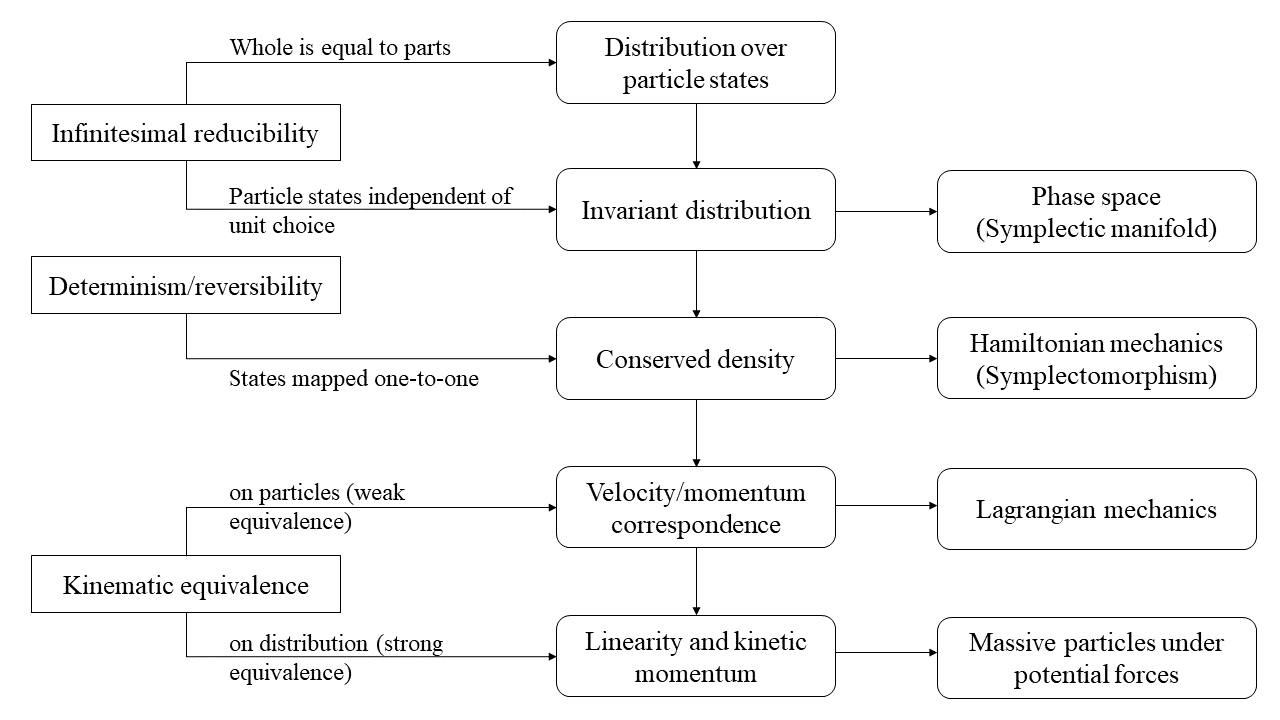
\includegraphics[width=\columnwidth]{images/ClassicalDiagram.png}
%	\caption{TODO: redraw this diagram in tikz and update outdated text}\label{fig_classical_diagram}
%\end{figure}

